\documentclass[fleqn,11pt, A4paper]{book}
%\documentclass[fleqn,11pt]{article}
%\documentstyle[olaf,11pt,fleqn]{article}
\usepackage{hyperref} % \href{}{}
\usepackage{verbatim}  % \verb;  ;
\usepackage{amssymb}
\usepackage{amsmath}
\usepackage{bbold}
\usepackage{graphicx}
\usepackage[pdftex,dvipsnames,usenames]{color}		% for pdf latex
%\usepackage{fancyheadings}
\DeclareGraphicsExtensions{.pdf,.png,.jpg}
%\input C:/OlafsUtil/LocalTex/lecture-w.sty
%\usepackage{C:/OlafsUtil/LocalTex/olaf2}
\long\def\Omit#1{}

\usepackage{filedate}
\usepackage{lineno}
\usepackage{subfig}
%\usepackage{titlesec}  % for paragraph sections
%\usepackage[utf8]{inputenc}


%\bibliographystyle{apalike}
%\bibliographystyle{abbrv}
\bibliographystyle{apsrev4-2}
%\usepackage{biblatex}
%\addbibresource{C:/Users/Olaf Scholten/Documents/AstroPhys/Lightning/Lght_papers/Olaf/LightningImagingRefs.bib}
%\addbibresource{../../../../Lght_papers/Olaf/LightningImagingRefs.bib}

%\let\tempone\itemize
%\let\temptwo\enditemize
%\renewenvironment{itemize}{\tempone\addtolength{\itemsep}{0.5\baselineskip}}{\temptwo}
\newenvironment{itemize*}%
  {\begin{itemize}%
    \setlength{\itemsep}{0pt}%
    \setlength{\parskip}{0pt}}%
  {\end{itemize}}
\newenvironment{enumerate*}%
  {\begin{enumerate}%
    \setlength{\itemsep}{0pt}%
    \setlength{\parskip}{0pt}}%
  {\end{enumerate}}

\def\beq{\begin{equation}}
\def\eeq{\end{equation}}
\def\bea{\begin{eqnarray}}
\def\eea{\end{eqnarray}}
\def\eqref#1{Eq.~(\ref{eq:#1})}
\def\eqlab#1{\label{eq:#1}}
\def\pdif#1#2{\frac{\partial #1}{\partial #2}}
\def\ddt{\frac{d}{dt}}
% figures
\setlength{\unitlength}{1.0cm}
\def\figref#1{Fig.~\ref{fig:#1}}
\def\figlab#1{\label{fig:#1}}  % Put in caption
%\@addtoreset{figure}{section}  % reset numbering for new (sub)section
%\def\thefigure{\thesection.\arabic{figure}} %compose fig. numbers

% Tables
\def\tabref#1{Table~\ref{tab:#1}}
\def\tablab#1{\label{tab:#1}}  % Put in caption
%\@addtoreset{table}{section}  % reset numbering for new (sub)section
%\def\thetable{\thesection.\arabic{table}} %compose equ. numbers

\def\secref#1{Section~\ref{sec:#1}}
\def\seclab#1{\label{sec:#1}}
%%%%%%%%%%%%%%%%%%%%%%%%%%%%%%%%%%55
%%% Use color for marking
\newcommand{\RED}{\color[named]{Red}}
\newcommand{\blue}{\color[named]{Blue}}
\newcommand{\red}{\marginpar{\RED\textbullet}\RED}
\newcommand{\m}[1]{{\marginpar{\RED\textbullet}\RED #1}}
\newcommand{\ToDo}[1]{{\marginpar{\RED\textbullet}{\bf \RED ToDO:} {\bf \blue #1}}}
\newcommand{\note}[1]{{\RED $\bullet$\ \bf #1 $\bullet$}}

\newcommand{\Olaf}{\color[named]{Purple}}
\newcommand{\os}[1]{{\marginpar{\Olaf Olaf}\Olaf\bf #1}}

%\newcommand{\thalf}{\mbox{\small{$\frac{3}{2}$}} }
\def\half{\mbox{\small{$\frac{1}{2}$}}}
\def\quarter{\mbox{\small{$\frac{1}{4}$}}}
\def\vslash#1{\mbox{/\llap #1}}    % p-slash
\def\ns#1{&\hspace*{-.35cm}#1&\hspace*{-.35cm}}
\def\newsub{\vspace*{0.1cm}
-------------------------------------------------------------------------------%
-------------------\\}
%\def\Var#1{{\textbf{#1}}}
\def\Subr#1#2{{\subsubsection{\tt{Subroutine #1}}\sublab{#2}}}
\def\subref#1{Subr.~\ref{sub:#1}}
\def\sublab#1{\label{sub:#1}}


\newcommand*{\FileDate}[1]{\expandafter\filedateX\pdffilemoddate{#1}\relax}
\def\filedateX#1#2#3#4#5#6#7#8{%X: |#1| |#8| \\
\filedateXX{#3#4#5#6}{#7#8}}
\def\filedateXX#1#2#3#4#5#6#7#8{%XX: [#1] [#8] \\
\filedateXXX{#1}{#2}{#3#4}{#5#6}{#7#8}}
\def\filedateXXX#1#2#3#4#5#6#7#8\relax{\formatdate{#1}{#2}{#3}{#4}{#5}{#6#7}}

\newcommand*{\formatdate}[6]{#1-#2-#3\ #4:#5:#6}

\def\ListInput#1\relax{
Source: \texttt{#1}; %Last edited: \FileDate{#1.tex}
%\input{#1}
}
%--------------------------------------------

%\pagestyle{fancy}
%\pagestyle{myheadings}
%\pagestyle{headings}
\renewcommand{\sectionmark}[1]{\def\naam{ #1}}
\renewcommand{\subsectionmark}[1]{\markright{\thesubsection.{\rm \naam}; {\sl #1} \hfill\today\hspace{1cm}}}
%\markright{\today \hfill
%     {\it \thesection , \arabic{section} \roman{subsection}
%      \hspace{1cm}}}

%\setcounter{secnumdepth}{4}
%\titleformat{\paragraph} {\normalfont\normalsize\bfseries}{\theparagraph}{1em}{}
%\titlespacing*{\paragraph} {0pt}{3.25ex plus 1ex minus .2ex}{1.5ex plus .2ex}
\makeatletter
\renewcommand\paragraph{\@startsection{paragraph}{4}{\z@}%
            {-2.5ex\@plus -1ex \@minus -.25ex}%
            {1.25ex \@plus .25ex}%
            {\normalfont\normalsize\bfseries}}
\makeatother
\setcounter{secnumdepth}{4} % how many sectioning levels to assign numbers to
\setcounter{tocdepth}{4}    % how many sectioning levels to show in ToC


%---------
\voffset-1.0cm
\textheight 22cm
\oddsidemargin 0.0cm
\evensidemargin 0.0cm
\textwidth 17cm

%%%%%%%%%%%%%%%%%%%%%%%%%%%%%%%%%%%%%%%%%%%%%%%
\begin{document}

\centerline{\LARGE \bf LOFLI}\vspace{2ex}
\centerline{\Large \bf LOFAR Lightning Imaging}\vspace{2ex}
\centerline{\Large Notes \& software description}\vspace{2ex}
\centerline{Olaf Scholten}\vspace{2ex}
\centerline{Kapteyn Institute \& KVI, University of Groningen, The Netherlands}\vspace{2ex}
\centerline{O.Scholten@rug.nl}\vspace{2ex}
\centerline{Source: \texttt{\jobname}; \hspace{3ex}
%Last Modified: \pdffilemoddate{\jobname.tex}\\
%\thepdfmoddateof{\jobname.tex}\\
Last edited: \FileDate{\jobname.tex} }\vspace{15ex}
\centerline{\Large  Guide to the LOFLI 2.0 program suite, V23}


\newpage

\vspace{2ex}
This guide is structured according to the chronological order of the main steps that are usually followed in converting LOFAR TBB data to an image of a lightning flash, with a chapter devoted to each subject. An outline of the basic imaging method can be found in \cite{Scholten:2021-init}.
Edition later than v21 contains also the routines for full interferometry (TRI-D imager).

In each chapter contains a description of the essential ingredients of the code, examples of input lines, examples of generated output, as well as examples of shell commands for running the code in Linux.

The code is free to be used, however it is requested to cite the publication where the features of the code are introduced and/or cite the software archive from where the code can be downloaded, \href{https://zenodo.org/records/4707495}{ZENODO} or the \href{https://github.com/OlafScholten/LOFLI/tree/LOFLI2.0}{LOFLI2.0 github repository}.

\newpage

\tableofcontents

%\newpage

\hfill \today

%\Omit{
\chapter{General Introduction}


\section{Installation cookbook for LOFLI-2.0}

The package operates on Linux as well as Windows platforms. Since, in my own installation, the main working horse operates only on the Linux system, where the main data archives are directly connected to, the Linux system is preferred and tested best.

Throughout a naming convention is followed (newly introduced in November 2023, attempting to be consistent) as outlined in \tabref{Naming}.

\begin{table}[!ht]
\caption{Naming conventions. \tablab{Naming}}
\begin{tabular}{|l p{14cm}|}
\hline
LL\_Base & The main installation folder (short for Lofar Lightning imaging Base folder).
\\& This should be set in {\small \verb!.bashrc! } (Linux) or for Windows in the Environment variables.
\\FlashFolder & one for each flash, named with the tag of the flash as for example in:
\\&  {\small \verb!FlashFolder=``/MainDir/18D-1"! }
\\ArchiveDir & The path to the archive containing the .h5 time traces from all antennas for a flash. If these reside on a remote site it is advised to use a SSHFS link through a local directory, as for example:
\\ &  {\small \verb!ArchiveDir=``/home/olaf/kaptdata/lightning_data/2017/D20170929T202255.000Z"! }
\\LL\_bin & The folder containing the executables of the programs.
\\&  {\small \verb!LL_bin=${LL_Base}/bin! }
\\LL\_scripts & Folder containing useful scripts
\\&  {\small \verb!LL_scripts=${LL_Base}/scripts!}
\\\hline
\end{tabular}
\end{table}

There are several software packages that should be installed on your system to obtain maximal functionality.

\begin{table}[!ht]
\caption{Required packages. \tablab{Required}}
\begin{tabular}{|l p{14cm}|}
\hline
gfortran & gnu fortran compiler, present on most Linux systems.\\
& For Windows, download from: \href{https://sourceforge.net/projects/mingw/}{sourceforge mingw}.
\\fftpack & Basic FFT routines.  Source code is included in this distribution.\\
& Download from: \href{http://www.netlib.org/fftpack/}{FFTPACK}; the double precision version is used.
\\lapack & Advanced linear algebra routines.\\
& Present on Linux systems, for Windows, download from: \href{https://www.netlib.org/lapack/}{LAPACK}.
\\blas & Basic linear algebra routines.\\
& Present on Linux systems, for Windows, download from: \href{https://www.netlib.org/blas/}{BLAS}.
\\hdf5-fortran & Allows random access to compressed data files with \href{https://portal.hdfgroup.org/display/support}{.h5} extension.\\
& Download from: \href{https://www.hdfgroup.org/downloads/hdf5/}{Linux} and \href{https://support.hdfgroup.org/ftp/HDF5/releases/hdf5-1.6/hdf5-1.6.7/src/unpacked/release_docs/INSTALL_Windows.txt}{Windows}
\\
GLE & Principal plotting utility \cite{GLE}.\\
& Download from: \href{https://glx.sourceforge.io/index.html}{sourceforge}. The shortcut ``gle" should start running the gle program.
\\\hline
\end{tabular}
\end{table}
\clearpage

\subsection{Linux installation of LOFLI-2.0}

Start by setting the system variable {\small \verb!LL_Base! } to point to the folder where LOFLI will be installed. To do so, edit {\small \verb!.bashrc! } in your home directory and add a line like\\
{\small \verb!export LL_Base=/home/olaf/LOFLI! }\\
where you should be careful not to add spaces around the = sign.

\begin{itemize}
\item Unpack the zip file  \href{https://zenodo.org/records/7393903}{ZENODO} or upload from  \href{https://github.com/OlafScholten/LOFLI/tree/LOFLI2.0}{LOFLI2.0 github repository} in the folder where LOFLI will be installed. Here we name this folder ``LOFLI". It is important to keep the directory structure. This should give something looking like \tabref{DirStruc}.
\item Edit the file ``ShortCuts.sh" between the lines marked with {\small \verb!#####! } to make sure that all system variables point to the right folders. The lines before or after this block should not be edited.
\end{itemize}

\begin{table}[!ht]
\caption{Directory structure after complete installation should be like this. \tablab{DirStruc}}
\begin{tabular}{|l l | p{10cm}|}
\hline
{``LOFLI"} & &\multicolumn{1}{|l||}{The main software folder for the LOFLI package} \\
\hline
   & bin & containing the executables. \\
   & docu &  containing documentation files. \\
   & flash & containing templates for installing the various working directories by running ``NewFlash.sh" scripts. \\
   & FORTRANsrc & containing the FORTRAN source codes. \\
   & GLEsrc &  containing gle-scripts for making plots. \\
   & scripts & containing the various shell scripts used in the background for the different applications. \\
   & Antennafields & containing information on antenna positions and such. \\
   & AntenFunct & containing the tables that define the antenna functions (Jones matrix) for the antennas. \\
\hline
\end{tabular}
\end{table}

\subsection{Windows installation of LOFLI-2.0}

This installation is very similar to that for Linux, except for some `insignificant' differences as all scripts have the extension ``.bat" in stead of ``.sh"., using `$\backslash$' in stead of `/' for folders, and `\%...\%' for using environment variables in stead of `\${...}'. 

Start by setting the system variable {\small \verb!LL_Base! } to point to the folder where LOFLI will be installed. To do so, edit the system variables for your windows system. The instructions given in {\small \verb!ModifyingWindowsParameters.docx! } in folder `docu' tell you how to do so. Add a variable named ``LL\_Base" to point to the directory where the LOFLI package is installed, on my system:\\
{\small \verb!"C:\Users\Olaf Scholten\Documents\AstroPhys\Lightning\LOFLI"! }\\
where the surrounding double quotes are essential when you path includes spaces.
For the rest follow the Linux instructions for downloading of the LOFAR and other packages, keeping folder names. Then edit the file ``ShortCuts.bat" (note: NOT .sh!!) between the lines marked with {\small \verb!#####! } to make sure that all system variables point to the right folders. The lines before or after this block should not be edited.

In the following instruction ALWAYS substitute extension ``.bat" when the instruction mentions  ``.sh".


%\newpage
\chapter{Setup \& RFI mitigation}
%The LOFAR data files are written in \href{https://portal.hdfgroup.org/display/support}{HDF5} format and require the installation of \href{https://portal.hdfgroup.org/display/HDF5/HDF5+Fortran+Library}{HDF5 for Fortran}, see the \href{https://www.hdfgroup.org/downloads/hdf5/}{download page}. There is also a \href{https://support.hdfgroup.org/ftp/HDF5/releases/hdf5-1.6/hdf5-1.6.7/src/unpacked/release_docs/INSTALL_Windows.txt}{Windows installation} possible.

Running the LOFLI package assumes a particular sub-directory structure as well as some particular files is each folder where you work on one particular LOFAR-download (also called flas). The script \verb!"NewFlash.sh"! should be copied from the main LOFLI installation folder to the folder, called `MainDir', where you want to create the folder for analyzing your flash. Running this script creates the correct directory structure, copies the necessary files from the \verb!"LOFLI/flash"! directory to the required new ``FlashFolder" (requires some editing of the shell code), starts to run the RFI-Mitigation code in batch-mode, and starts an exploratory imaging run, see \secref{Explore}, of the data after the RFI-mitigation has finished.
When setup correctly ``FlashFolder"  has two subfolders named \verb!"Book! and \verb!"files!. The first will store the calibration files which are essential for imaging and the latter files needed for intermediate checking and it may be considered as a scratch directory. These directories as well as necessary script files are copied to their appropriate location by running the script \verb!"NewFlash.sh"! in the MainDir.

Best practise is to name the FlashFolder (as set in script \verb!"NewFlash.sh"!) with the tag of the flash, say \verb!"18D-1"!. Make sure this flash is correctly listed in file `list.ssv' residing in \verb!"LOFLI/scripts"!.
The translation from the shorter internal flash label used in the lightning group to the UTC-label used by LOFAR is generated by the script \verb!"FlashID.sh"! that resides in the Utilities directory. This script reads the file \verb!"list.ssv"! and make sure this is updated for your system, where the first entry is the short-hand notation used for the FlashFolder name and the third entry refers to the flash identifier used in the (LOFAR) archive.



In the script \verb!"FlashID.sh"! also \verb!ArchiveDir=/home/olaf/kaptdata/lightning_data/"! needs to be set to the proper place where the raw LOFAR-data reside. Note that there are no spaces allowed around the equal signs. The system variable ``ArchiveBase" as set in ``ShortCuts.sh" should point to the directory that contains the TBB data from LOFAR as .H5 files. It is very handy to make a sshfs logical connection between the remote computer containing the archive and a local folder if the archive is not on your local system already.



\section{RFI mitigation}\seclab{RFIm}

The purpose of \verb!"RFI_Mitigation.sh"! is to pre-process the data-files for a single flash and in the process determine the frequency notch filters to mitigate RFI. The RFI filter data is written to \verb!"Book/RFI_Filters.uft"! of the main flash-working directory `FlashFolder'. The file names to be processed are read from the file \verb!"directory.out"! (should be in the FlashFolder) as was created by the script \verb!"NewFlash.sh"!. The script \verb!"NewFlash.sh"! should have automatically started the running of \verb!"RFI_Mitigation.sh"!.


The files will be processed in the order as listed in \verb!"directory.out"!
where the \note{ second } station in the directory listing will be used as the reference station later in imaging (to change this replace the ``2" on the line \verb!"${ProgramDir}$Prog ${AntennaFieldsDir} 2"! by the appropriate number in \verb!"RFI_Mitigation.sh"!). Be careful to set here a station that is in a rather dense part of the array, preferably be it  CS002.

Additional axillary information needed for the imaging runs is written to\\ \verb!"Book/LOFAR_H5files_Structure.dat"! .

The script \verb!"RFI_Mitigation.sh"! takes a while to run. At the end it will submit the script \verb!Explore.sh!.


\subsection{Additional details}

All files in the directory listing given in \verb!"'directory.out'"! are scanned. If 9 of the first 100 data-chunks of a specific antenna are non-zero an RFI analysis is made otherwise the antenna is omitted from further analysis. The amplitudes of the 9 frequency spectra are summed. In the range of 25 to 79~MHz. A running (inclined) straight line fit is made over 2~MHz. When the amplitude is larger that the average (from the line-fit) that frequency is filtered out. In addition the power in this frequency range is determined as the sum of the square amplitude (in frequency). This power will later be used to normalize spectra. The antenna positions are obtained from the files in directory \verb!"AntennaFields/"! (in ``MainDir") and written to the auxiliary file.

\subsection{Figures and print-out}\seclab{RFI-out}


\begin{figure}[th]
\centering{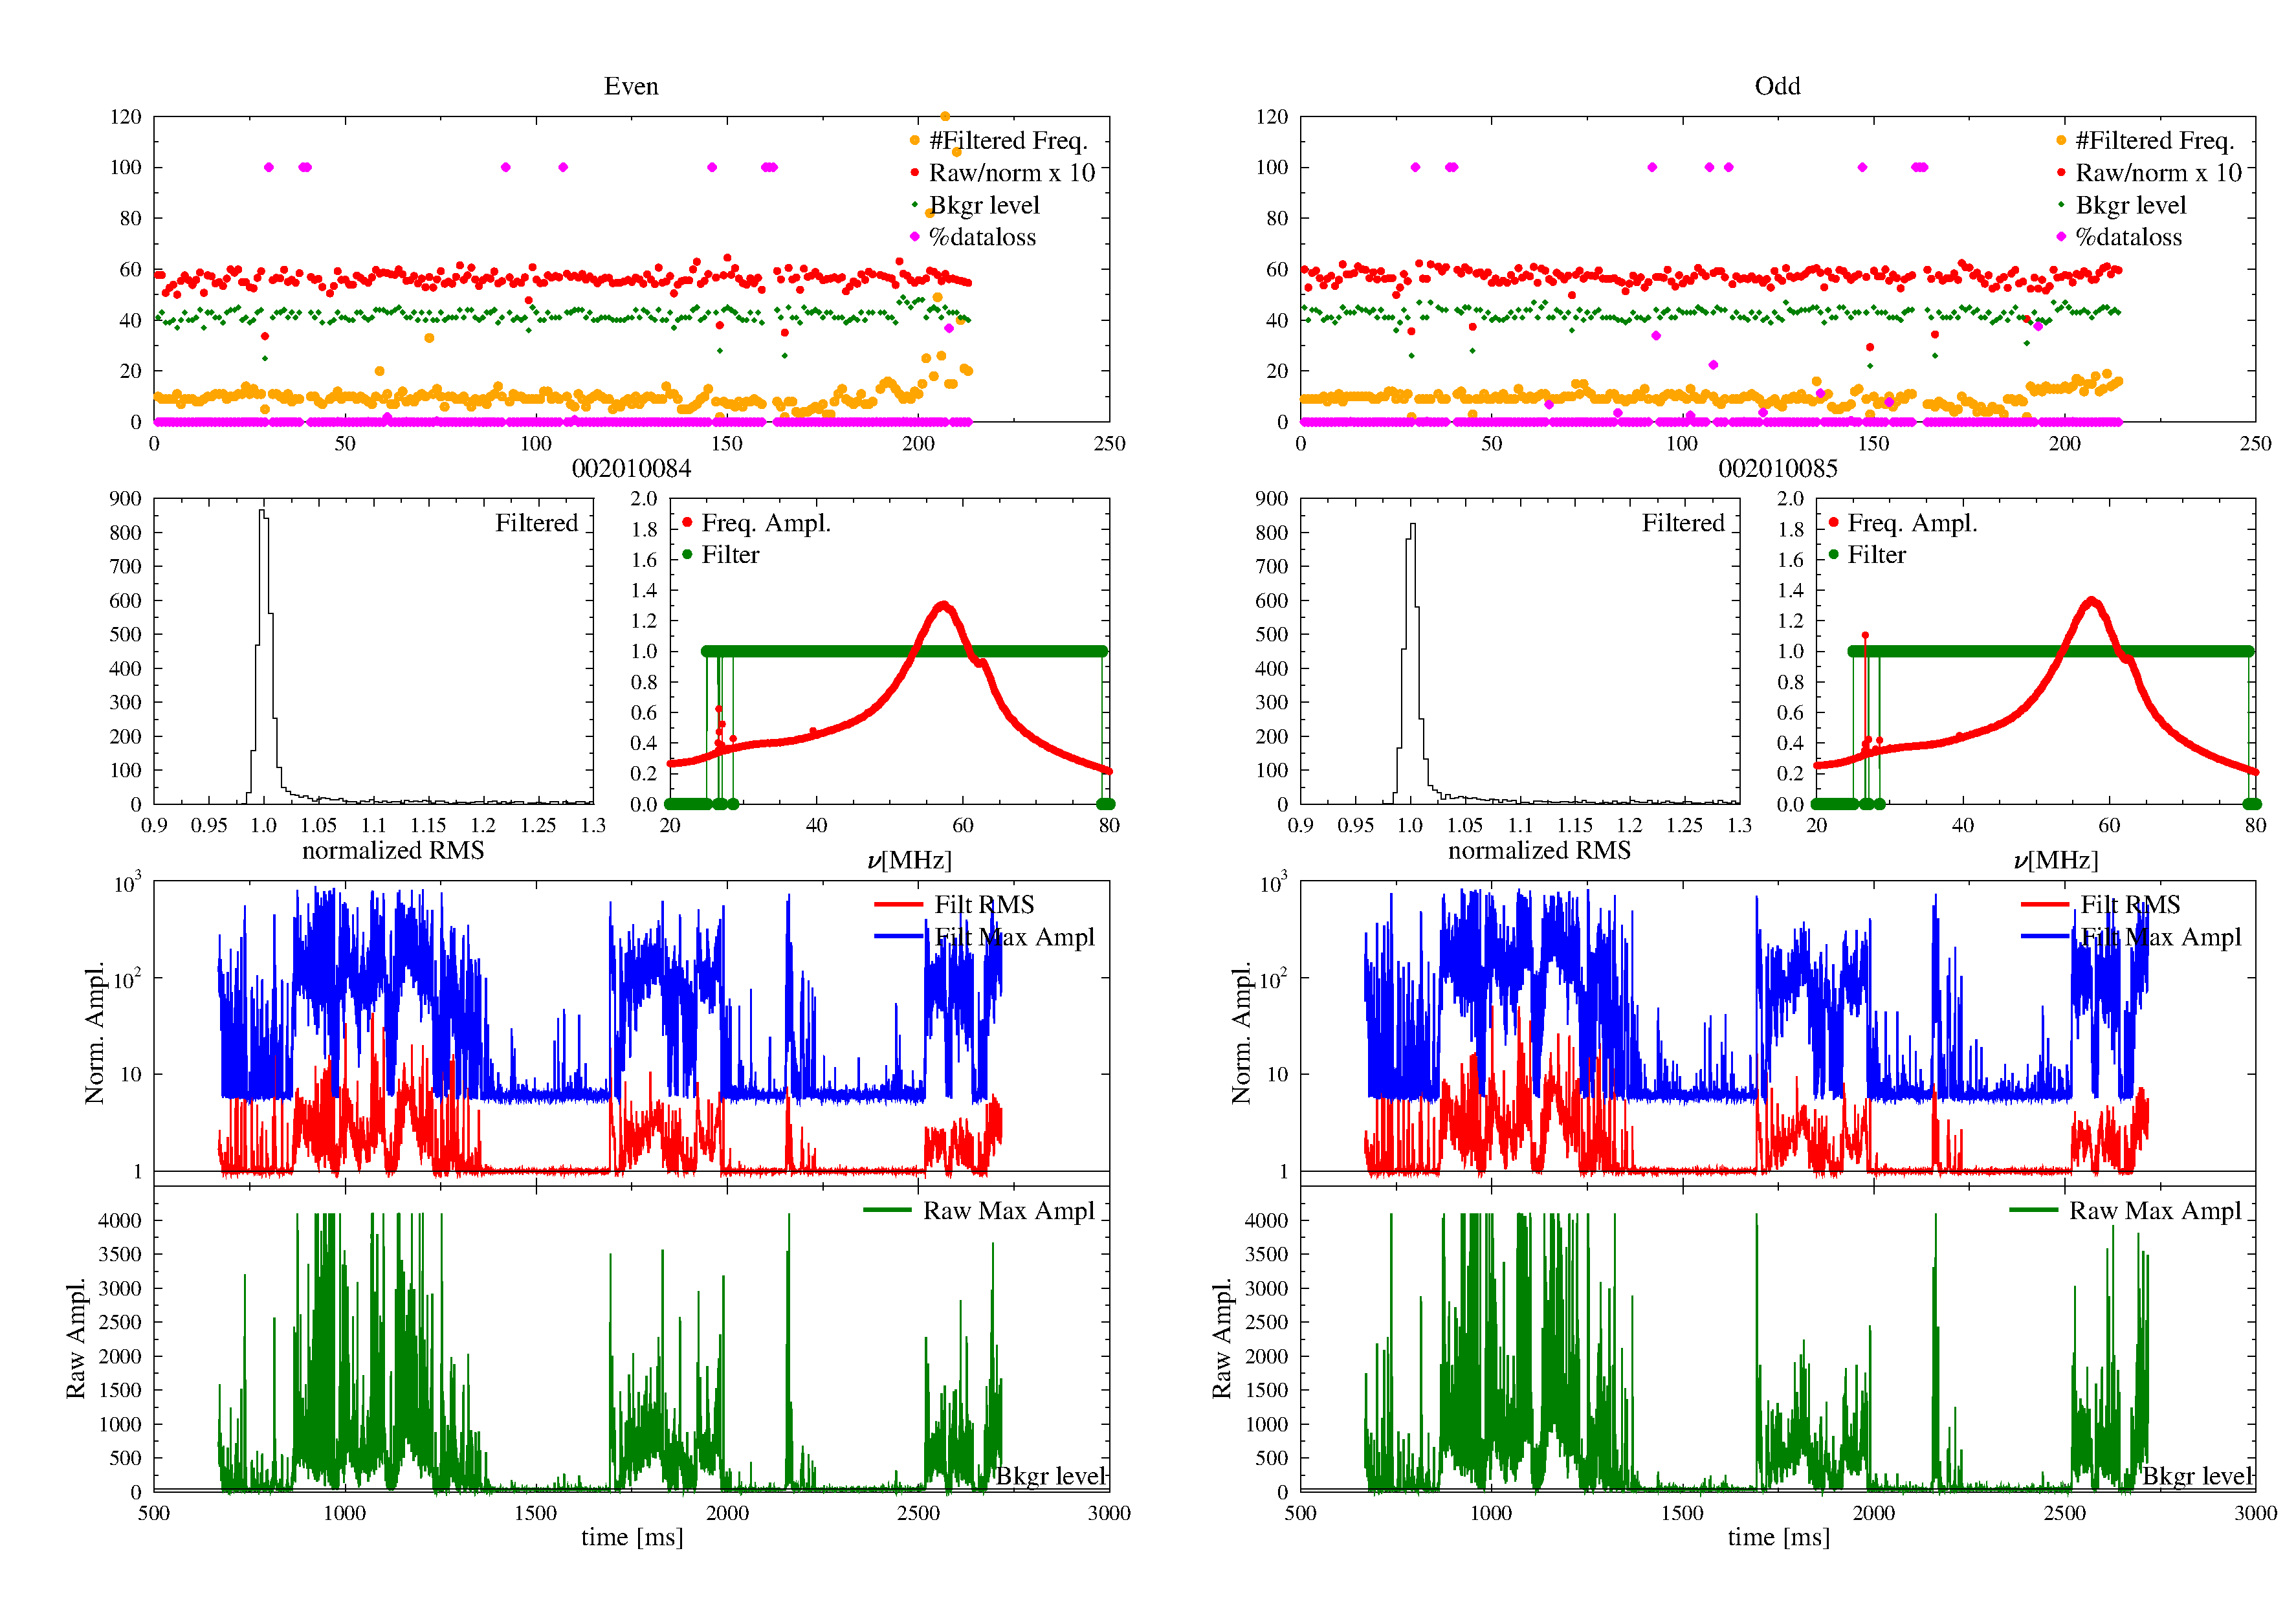
\includegraphics[width=0.89\textwidth]{Figs/RFI_Plots-20A7} }
%\centering{\includegraphics[ bb=1.0cm 2.4cm 24.5cm 25.7cm,clip, width=0.49\textwidth]{../Figs/SE20A7-NPMx_1HIntfSpecSel} }
	\caption{RFI plot results result for a typical flash, 20A-7 in this case.}	 \figlab{Intf-NLaH}
\end{figure}

In \figref{Intf-NLaH} a typical plot is shown as generated by the RFI-mitigation program. The results are presented separately for Even- (odd-) numbered antennas officially known as Y- (X-)dipoles. The to panel shows for each antenna (over 200 even and odd antennas for this case). For all values it is important that it does not vary too much, where outliers need to be scrutinized.
\begin{description}
\item[orange] The number of notch filters to mitigate RFI within the specified frequency band (30-80~MHz). The RFI filters are determined per antenna and taken the same for all data-chunks.
\item[red] The normalization factor between raw data and the noise-normalization.
\item[green] For every chunk of data (0.3~ms) the maximum amplitude is determined. The minimum value for all chunks of these maxima/chunk, a measure of the background, is shown.
\item[magenta] The percentage of data chunks that have too much data loss to be considered in the analysis.
\end{description}
The panel ``Filtered'' gives the Distribution of mean power (square of the complex amplitude) after filtering per chunk for all chunks in the reference station.
The panel next to it gives the frequency filter (for the reference station) in green and the antenna gain in red.

The bottom panels give, again for the reference antenna, for each chunk, the RMS power after RFI filtering (the same data as used in making the plot in panel ``filtered''), and the maximum amplitude (blue: after filtering, green: before filtering). This gives a good indication of the time-frames with lightning activity. Note that for this example the reference antenna had no data loss, if it had, the blue line would go to the bottom of the panel for the chunks with data loss.

Part a typical output (the .out file) that contains useful info for further imaging (the non-diagnostic part).

\begin{linenumbers}
\tiny
\resetlinenumber
\begin{verbatim}
 time range for which there are data [ms]   669.00223999999992        2717.0073600000001
 !!!!!!!!! For           22  Antennas RFI-mitigation failed, out of a total of         427  !!!!!!!!!!!!
        5094        5095        7093       11088       11089       11090       11091       13088       32086       32087      103092      103093      121091      125088      125089      130092      130093      130094      130095      145088      145089      166094
 MinAmp statistics:   41.883950617283951        41.991680539934350
 statistics powr=sq(raw/Norm):   31.767085498017074        31.995666167967695
 !!!!!!!! Bad antenna based on Raw Amplitude range        5092          25   32.866010868572779        50.901890365995122
 !!!!!!!! Bad antenna based on powr        5092          11
 !!!!!!!! Bad antenna based on Raw Amplitude range        5093          26   32.866010868572779        50.901890365995122
\end{verbatim}
\end{linenumbers}

This summary lists the antennas that are -most likely- better be omitted from subsequent analysis. Given is the Station Antenna ID (SAI) number that is used internally in the analysis code. The translation table from station ID to station Mnemonic is
{
\tiny
\begin{verbatim}
       1     2     3     4     5     6     7    11    13    17    21    24    26    28    30    32   103   106
   CS001 CS002 CS003 CS004 CS005 CS006 CS007 CS011 CS013 CS017 CS021 CS024 CS026 CS028 CS030 CS032 CS103 RS106

     121   125   128   130   141   142   145   146   147   150   161   166   167   169   181   183   188   189
   CS201 RS205 RS208 RS210 CS301 CS302 RS305 RS306 RS307 RS310 CS401 RS406 RS407 RS409 CS501 RS503 RS508 RS509
\end{verbatim}
}
The (most often) long line with numbers are the SAI of stations where the RFI-suppression filter could not be determined due to too much data loss. The following lines give the SAI of the antennas that are suspect because the power-normalization was outside reasonable bounds (red dots in top panels of \figref{Intf-NLaH}), or because the amplitude range was off (green dots in \figref{Intf-NLaH}).

At the very end of the output lines are printed resembling
\begin{linenumbers}
\tiny
\resetlinenumber
\begin{verbatim}
 BadAnt_SAI=   3048,   3054,   3055,  13090,  21049,  24062,  26054,  32049,  32072, 161084
             181055, 106063, 130049, 130063, 130091, 145048, 145054, 145084, 146072, 169072
             188049, 188091, 189054, 189084,
\end{verbatim}
\end{linenumbers}
giving the estimate of the program for the bad antennas. These lines may be copied into the namelist input for the analysis program as described in \secref{Image}. 
\clearpage
\chapter{The LOFAR Imagers}\seclab{Image}
The main imaging 'work horse' is the code ``LOFAR-Imag". It can be run with several different flavors that are described in \secref{Explore} till \secref{E_Intf}. The general structure of the  input is (as specified in a plain text file with extension .in)
\begin{linenumbers}
\resetlinenumber
\begin{verbatim}
&Parameters
p=v
p=v
&end
- - - - -- - - -- -
specific input lines
\end{verbatim}
\end{linenumbers}

where  \verb!p=v! stands for a list of parameters that are assigned a value (the so-called "namelist" input part). A list of the possible parameters with the first section where they are described is given in \tabref{LOFLI-namelist}. Some of these parameters apply to (practically) all run-options and are described here, many others are more specific and will be described in the appropriate section.

The namelist parameters that are general are the following,

\begin{linenumbers}
\resetlinenumber
\begin{verbatim}
 &Parameters  RunOption= "xxxxx"
 OutFileLabel= "xx"
 AntennaRange= 100.  ! Maximum distance (from the core) for the range of the antennas (in [km]).
 SaturatedSamplesMax= 5     ! Maximum number of saturates time-samples per chunk of data
 Calibrations= "Calibrations202202071319.dat"     ! The antenna time calibration file. Not used when running on simulated data!
 SignFlp_SAI= 142092, 142093     ! Station-Antenna Identifiers for those where the sign of the signal should be reversed.
! PolFlp_SAI=  0     ! Station-Antenna Identifiers for those where the even-odd signals should be interchanged.
 BadAnt_SAI= 5095, 7093, 11089, 13088, 13089, 17084, 17085, 17094, 17095, 101085
  141083, 141086, 141087, 167094, 169082, 169090, 169094     ! Station-Antenna Identifiers for those that are malfunctioning.
 ExcludedStat= "RS305"     ! Mnemonics of the stations that should be excluded.
&end
\end{verbatim}
\end{linenumbers}
where more parameters from \tabref{LOFLI-namelist} may be added. All text on a line after an exclamation mark is considered comment and not used. The following lines are obtained from experience with other flashes, where:
\\\verb!RunOption="xxxxx"! specifies the particular flavor of the program that should be used, where "xxxxx" can be any of the following:
\begin{itemize}
\item \verb!RunOption="Explore"! for first exploration of this flash in order to get some idea of the layout and timing, see \secref{Explore}.
\item \verb!RunOption="Calibrate"! for performing time calibration using the Hilbert envelopes of the cross correlations, see \secref{Calibration}.
\item \verb!RunOption="ImpulsiveImager"! for running the impulsive Imager, see \secref{Imag}.
\item \verb!RunOption="FieldCalibrate"! Field Calibration for the TRI-D interferometric imager, see \secref{Intf?}.
\item \verb!RunOption="TRI-D"! for the TRI-D imager with polarization observables, accounting for antenna function, see \secref{Intf}.
\item \verb!RunOption="SelectData"! to select real data, possibly for setup of simulation runs using program "SimulateData", see \secref{SelDat}.
\end{itemize}
\verb!OutFileLabel= "xx"! specifies an identifier for this particular run. It will be included in the name of the text-output file (with extension .out), as well as any figures (.pdf) and data files (.csv or .dat).
\\\verb!AntennaRange= 100.! Maximum distance (from the core, in [km]) for  antennas to be included in the calculations. Only in the "Explore" runoption this variable is not used.
\\\verb!SaturatedSamplesMax= 5! specifies the maximum number of time-samples in a data chunk (block of time trace) where the LOFAR digitizer has saturated.
\\\verb!Calibrations= "......"! points to a calibration file in the sub-folder \verb!Book! that was produces in an earlier calibration run, see \secref{Calibration} and/or  \secref{Intf}.
\\\verb!SignFlp_SAI=! list the antenna IDs where the signal is reversed.
\\\verb!PolFlp_SAI=! list the antenna IDs where the polarization is reversed.
\\\verb!BadAnt_SAI=! list the antenna IDs where the signal is bad.This line may be copied from the output of the RFI mitigation run, see \secref{RFI-out}.
\\\verb!ExcludedStat=! lists the stations that should be excluded from the calculations.
\\ Note that none of these lines in the namelist have a comma at the end, for the other input lines this is optional. Several keywords may appear on a single line if separated by a comma. Anything after an exclamation mark (within the namelist) is treated as a comment. A complete list of namelist keywords is given in \tabref{LOFLI-namelist}.



\clearpage
\section{The `Explore' option}\seclab{Explore}

For the time-calibration we will use a boot-strap method that necessitates the use of some strong pulses for this particular flash. To locate these the program needs to run the script \verb!Explore.sh! (run automatically after RFI-suppression) where the input options are read from the file \verb!"Explore.in"! in the FlashFolder. Typical input lines are

\begin{linenumbers}
\resetlinenumber
\begin{verbatim}
&Parameters
 RunOption= "Explore"
 Calibrations= "Calibrations_ZERO.dat"
! ExcludedStat= "RS210", "RS310", "RS208", "RS409"
 SignFlp_SAI=   21078, 125028, 142092, 142093, 145032, 145033, 166015
 PolFlp_SAI=   021092,  30028,  32092, 106044, 106064, 125028
               145032, 146092, 166014, 181048, 181092,  189076
 BadAnt_SAI=   003065, 021078, 021079, 021093, 026030, 32016, 32017, 32048, 32049
               101045, 125029, 150065, 188051, 188094, 188095
               31086,  31088, 31071
&end
- - - - -- - - -- -
\end{verbatim}
\end{linenumbers}
using the minimal number of input parameters. For the exploratory search of the flash only the antennas within 2.5~km from the core are used.

The program will produce a file in the FlashFolder \verb!"Explore.out"! that has diagnostic information. The script will also produce a plot \verb!"Map_Explore.pdf"! that gives an overview of the image at 30~ms time steps.

\subsection{Figures and print-out}\seclab{Expl-out}

\begin{figure}[th]
\centering{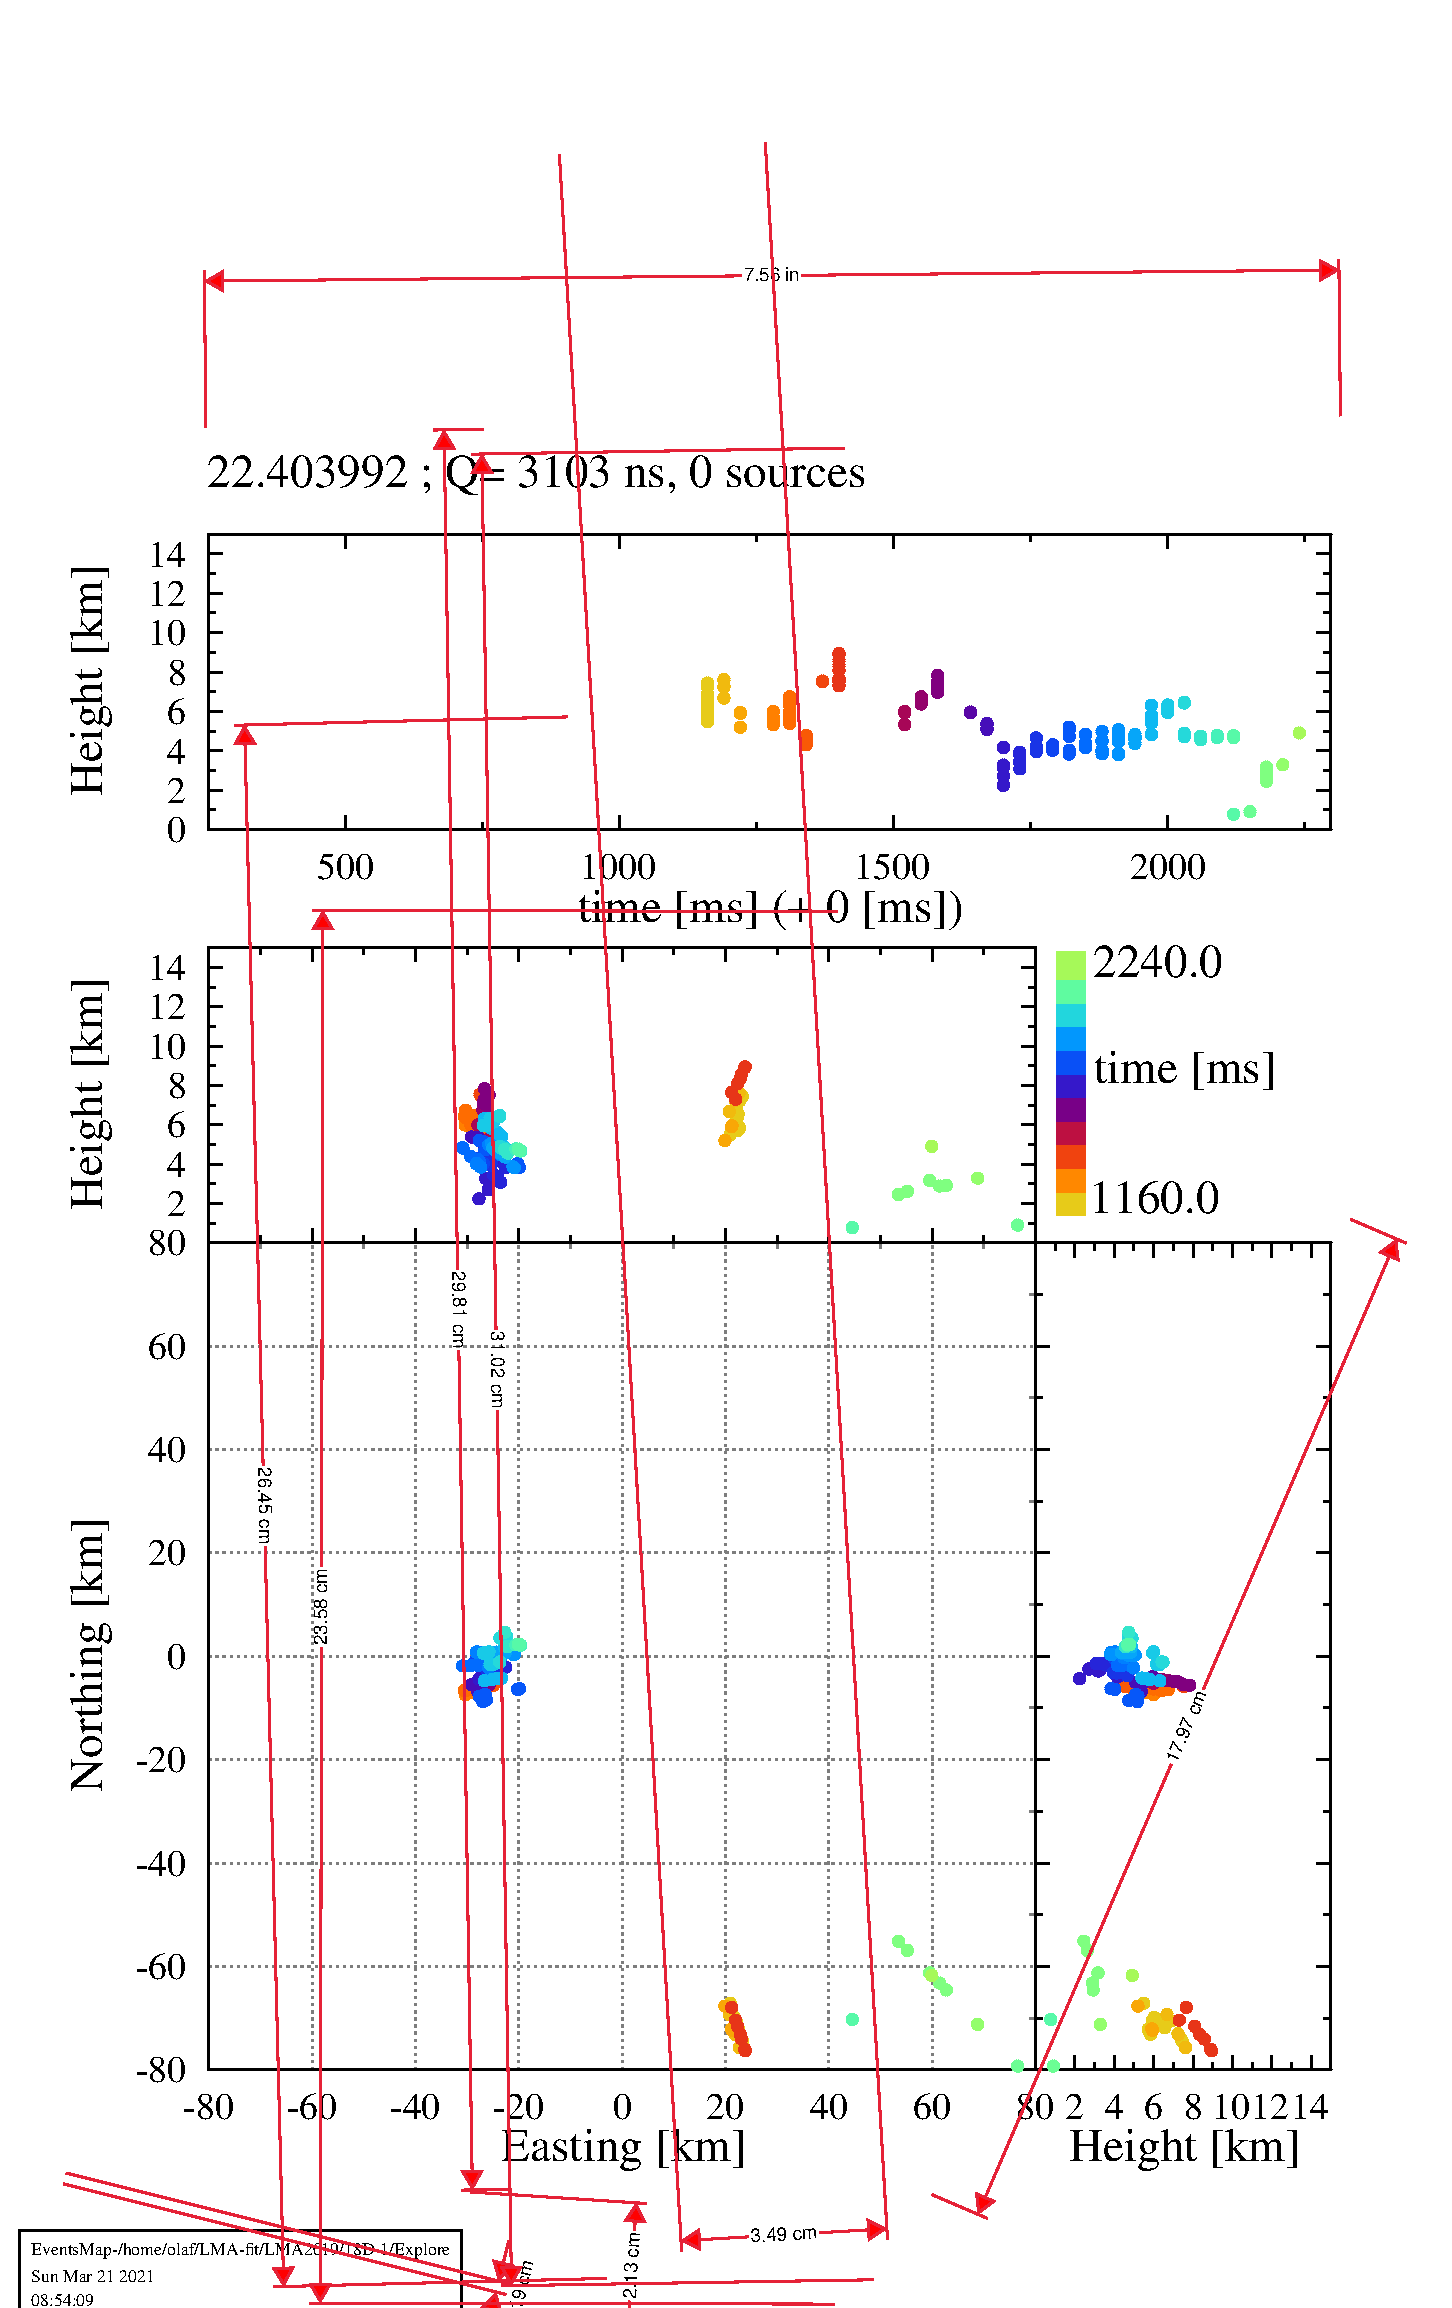
\includegraphics[bb=0cm 0cm 25.5cm 31.4cm,clip, width=0.49\textwidth]{Figs/Map_Explore-18D1} }
%\centering{\includegraphics[ bb=1.0cm 2.4cm 24.5cm 25.7cm,clip, width=0.49\textwidth]{../Figs/SE20A7-NPMx_1HIntfSpecSel} }
	\caption{Exploratory view of Flash 18D1, showing the areas and periods of lightning activity.}	 \figlab{Expl-Fig}
\end{figure}

At the end of the ``explore'' run a plot is made that should resemble \figref{Expl-Fig} giving a rough idea of the spatial and temporal extent of the flash.



\section{The `Calibrate' option}\seclab{Calibration}

This option is used to perform the time-calibration of all antennas and antenna stations.

The calibration is run from the script \verb!"Calibrate.sh"! where the input is set in the file \verb!"Calibrate.in"!. The calibration script has to be run many times over, first to obtain sources of sufficient quality (stand alone, little interference with others, similar structure for all antennas, visible in even and odd numbered antennas) using calibration files from another flash, followed by runs where the antenna calibration is fixed at the nanosecond level.  The scripts need to be run in the FlashFolder.

The general philosophy is to select a few of the strongest pulses in different parts of the lightning discharge. These should cover the spatial extent of the flash reasonably well. The exploration map, see \secref{Explore}, is a good tool to select times at which to search for the good sources for time calibration.
Pulses located in a few independently selected chunks of data on the reference antenna should be fitted simultaneously, i.e.\ fitting simultaneously all source locations as well as station and antenna timings.

The different steps in calibration are
\begin{enumerate}
\item Find calibration source that are spread reasonably homogeneously over the complete extent of the storm.
\begin{enumerate}
\item Either from 'Explore.out' or from 'Img\_Explore.pdf' find the times for which the active regions in the storm covers all areas.
\item For each of these times run the imager (using the calibration from another flash) for a time span of -not more- than 1~ms with an input line like
{
\tiny \begin{verbatim}
   948  , 11900.  -26204.    5950.   , 0 1.
\end{verbatim}
}
and it will generate a file named 'Srcs22-5star-$\cdots$.dat'.
\item Cut a section from this 5star file that resembles

\begin{linenumbers}
\tiny
\resetlinenumber
\begin{verbatim}
    974.771040      15.70      -1.85       7.53  4479001
C 2 2 1   38719  10064.73,  -5428.98,  11197.11,     0.97491;    0.417,  0.7154,  0.4560,  0.8930,  31,  38,   3361,  8, 10,  0
C 9 2 1   40061  15720.37,  -1856.59,   7545.11,     0.97491;   23.390, 19.5381, 10.0996,  9.3094,  31,  38,   1423,  9, 10,  0
C 1 2 1   15254  15550.96,  -1838.29,   7466.56,     0.97479;    4.493,  0.1831,  0.3413,  0.6994,  30,  30,   5921,  6, 15,  1
C 8 2 1   39836  15515.73,  -1860.96,   7448.69,     0.97491;   13.274, 15.2286,  7.8900,  7.4356,  25,  30,   1549, 10,  6,  1
\end{verbatim}
\end{linenumbers}
and paste this in the input of 'Calibrate.in' which should now look like what is shown in \secref{Fcal}. Make sure that the location specifies in the chunk line (starting at t=974.771040~ms for this case) is pointing to the right general direction. The coordinates of (N,E,h) may all three be specified in units of m or km, whichever you prefer.
\item At this stage I found it more efficient to work on each chunk separately.
\item Check the generated curtain plots carefully. 1) Make sure the pulse in the reference station is reasonably well separated from others and is not wide. 2) The pulse is seen in even and odd antennas. 3) mark for exclusion those stations for which the pulse differs from what is seen in the reference antenna. The resulting input should resemble what in given is \secref{Scal}.
\item Run the case of \secref{Scal} a few times until the chi-square per degree of freedom for each source (as listed at the end of the 'Calibrate.out' file) is reasonable, typically below 5 or 10. When there are sources that are notoriously bad, omit them from the calculation. It may be useful to check .out file for the contributions of each station to the chi-square of each source. Listed are the mean time difference and the standard timing error for a station. If one of these is large, check the curtain plot for the reason and use this to base your decision to mark a station for exclusion.
\item Repeat these steps for a few different chunks until you have covered the complete extent of the storm.
\end{enumerate}
\item Combine all calibration sources in one calibration run, where each chunk line is followed by lines with the sources and excluded antennas. The input should resemble what is given in \secref{Scal}.
\item Run this while fitting all station timings as well as source locations as specified by the line
{
 \tiny \begin{verbatim}
abut  !
\end{verbatim}
}
where there should be no leading spaces. In the namelist set ' WriteCalib=.true. ,' and possibly ' FitRange\_Samples=10 ,'. On the basis of the result you may want to exclude (or include again) some stations, but always consult the curtain plots. If so, re-run. Always copy the chunk and source lines at the end of the .out file into the .in file and cut and paste the calibration line into the namelist of the .in file.
\item Next is to fit the antenna timings within a station. To do so replace the 'abut' line with
{
\tiny \begin{verbatim}
antenna RS106 RS205 RS208 CS301  RS306 RS307 RS310 RS406 RS409 CS501 RS508 RS509 NoSrc !
\end{verbatim}
}
where you list the stations for which the antenna timings could use adjustment. Experience tells that about 12 stations is the max the program can handle when using 'NoSrc', specifying that the parameters of the sources are not varied during the search. The program will protest if the number is too large.
\item Repeat this for all stations. Cut and paste the name of the generated .cal file to the input for the next run.
\item After adjusting the timings of the antennas within each station, the timing standard deviation per station and per source should be order 1~ns or less. To guarantee this (and allow some lee-way put ' StStdDevMax\_ns=2. ,' in the namelist input. This will mark for exclusion all stations for which this value is exceeded. Probably repeat the antenna calibration runs.
\item Check in the process that for each station there are a sufficient number, typically 5) of calibration sources left (for each orientation). If the number is smaller, either find more possible calibration sources (i.e. go to the beginning of this recipe) or exclude the station from the analysis (and later imaging). This may happen if the station is at a too large distance from the source region and thus has a -comparatively- high noise level.
\item Use again the option 'abut !' to make a final station timing and calibration source adjustment.
\end{enumerate}

Added notes:
\\1) It is more efficient to replace step 1b by en earlier imaging of the complete flash with an approximate calibration and to select for step 1c the appropriate parts of the long 5star file that was generated in the imaging of the complete flash. Note that the generated image is probably poor (do use ' AntennaRange=100').
\\2) In step 1d care should be taken that at the end of the procedure a pulse is seen (or is likely hidden in the noise) for all antennas (even if they are too noisy or messy to include in the calibration) at the expected position. If not this implies that the source location must be off and thus this peak will not contribute to a reliable calibration. To steer the source-position search play a bit with 'FitRange\_Samples' since this variable sets the range from the expected position where pulses may be included in the search. It requires some trial-and-error to get a 'feel' for this variable. Its value is very important so pay attention!


\subsection{First calibration stage}\seclab{Fcal}

For the first run the typical content of \verb!"Calibrate.in"! is like

\begin{linenumbers}
\tiny
\resetlinenumber
\begin{verbatim}
&Parameters
 RunOption='Callibrate'
 CurtainHalfWidth=100  !
! XcorelationPlot=.true. ,
! FullAntFitPrn=.true.
 AntennaRange=100
 FitRange_Samples=20
 SaturatedSamplesMax=3 ,
 StStdDevMax_ns=20. ,
! WriteCalib=.true.
!  Calibrations="Hil21C-3-202204260923.cal" ! Hilbert T  1.44 antenna
  Calibrations="Hil21C-2-202204262256.cal" ! Hilbert T  6.48
 SignFlp_SAI=  142092, 142093
 PolFlp_SAI=  32086,
 BadAnt_SAI=   003065, 021078, 021079, 021093, 026030, 32016, 32017, 32048, 32049,
               101045, 125029, 150065, 188051, 188094, 188095
! OutFileLabel="T"
&end

    974.771040      15.70      -1.85       7.53  4479001
C 2 2 1   38719  10064.73,  -5428.98,  11197.11,     0.97491;    0.417,  0.7154,  0.4560,  0.8930,  31,  38,   3361,  8, 10,  0
C 9 2 1   40061  15720.37,  -1856.59,   7545.11,     0.97491;   23.390, 19.5381, 10.0996,  9.3094,  31,  38,   1423,  9, 10,  0
C 1 2 1   15254  15550.96,  -1838.29,   7466.56,     0.97479;    4.493,  0.1831,  0.3413,  0.6994,  30,  30,   5921,  6, 15,  1
C 8 2 1   39836  15515.73,  -1860.96,   7448.69,     0.97491;   13.274, 15.2286,  7.8900,  7.4356,  25,  30,   1549, 10,  6,  1
- - - - -- - - -- -
only !
\end{verbatim}
\end{linenumbers}

The order of the parameters in the namelist input is arbitrary. All input on the line after an exclamation sign (!) is ignored and may be used for comments, or storing parameter one may want to use on some other run. Some of the parameters were explained already and the new ones (labeled by line number) are:
\begin{enumerate}
\item[3] \verb#"! CurtainHalfWidth=100"#: curtain plots (see \secref{CurtainPlot}) are made for each calibration source with the specified width (in time samples of 5~ns). No plots are made when the width is zero or negative (default).
\item[4] \verb#"! XcorelationPlot=.true."#: No plots of the cross correlations (see \secref{XCorPlot}) are made since the default for this variable is .false..
\item[5] \verb#"! FullAntFitPrn=.true."#: No extensive printout giving the time offsets per antenna per source (see \secref{PrintOut}) is made since the default for this variable is .false..
%\item[6] \verb#"! FitIncremental=.false."#: Since the default for this variable is .true. antennas within an increasing range around the core will be included in the source locating fits, where the source locations of the previous fit are used as the guess locations for the following iterative fit in which more distant antennas are included.
\item[6] \verb#" AntennaRange=100"#: All antennas within a distance of 100~km from the core will be included in the calculations.
\item[7] \verb#" FitRange_Samples=20"#: The maximal range, in samples (of 5 ns), that is searched for a pulse around the predicted location (based on the pulse location guess). The range may be made smaller if the error on the guess location is small. In a first run the value for \verb!FitRange_Samples! should be relatively large to be able to find peaks also for antennas that are very poorly calibrated. Later in the calibration process it will be tuned down.
%\item[8] \verb!" Dual=.false."!: The peaks in even and odd numbered antennas will be searched for independently. In a later round the two will be coupled.
\item[8] \verb#" SaturatedSamplesMax=3"#:  Maximum number of saturates time samples per chunk of data. 3 may be a bit conservative.
\item[9] \verb#"! StStdDevMax_ns= 20 "#:  Stations are excluded when the standard deviation in antenna-arrival times for a pulse in one station exceeds this value.
\item[10] \verb#"! WriteCalib=.true."#: The obtained new antenna calibrations (if calculated) will not be written to an updated calibration-data file.
\item[20] \verb#"      974.771040      15.70      -1.85       7.53  "#: A chunk-specification line. In this example a single one, but the number is free. It specifies the time-slots where pulses should be searched as well as the general expected location of the sources. Separating commas are not necessary. These times and locations are obtained from the earlier Explore run. It is recommended to stay below 5 entries. The experience is that it is easier to try different sections of the flash in separate runs.
    \begin{description}
    \item[974.771040] The data chunk of 0.3~ms length starting at this time (in [ms]) will be used.
    \item[15.70      -1.85       7.53] The position (N,E,h)  that is taken as a first guess for the source positions (specified in either [m] or [km], a mix is not allowed). The location should be in the right quadrant, but not more precise. Note that the first character on the line should not be left as a space.
    \end{description}
\item[21 $\cdots$ 24] \verb#"C 9 2 1   40061  15720.37,  -1856.59,   7545.11, "#: Specification of the peaks that should be considered. For this example this line was cut\&paste from 'Srcs22-5star-.dat', which appears more efficient. The lines can also be omitted and some candidate sources will be searched. Note that the formatting of this line is very important.
    \begin{description}
    \item[C] the sample number of the peak is given as if the antenna were right at the core.
    \item[ 9] The 9$^{th}$ pulse as found by the imager. This number is not used, but may be good for your own bookkeeping.
    \item[ 2] The same source is used for even and odd numbered antennas. Note that all should be labeled with with '2' or none, no checking is done. Alternatively it is possible to specify even ('0') and odd ('1') antennas separately, see \secref{Scal}.
    \item[ 1] The chunk number.
    \item[ 40061] The sample number specifying the location of the peak on the time trace.
    \item[15720.37,  -1856.59,   7545.11] The position (N,E,h) in [m] that is taken as a good guess for the source position.
    \end{description}
\item[25] \verb#" - - - - -- - - -- - "#: A closing line as long as it does not contain a line with number, but only text.
\item[26] \verb#"only !"#: No search for antenna calibrations is done at this stage, source locations only.
\end{enumerate}

Running the script \verb!"Calibrate.sh"! for this input file goes fast and will crate the files  \verb!"Calibrate.out"! with much diagnostics concerning the fit results for all sources as well as a series of plots, see \secref{Cal-out}.

\subsubsection{Discussion}

In calibrating one should use the stronger sources (seen in more antennas), narrow pulses (better timing resolution since extended sources have some intrinsic resolution), and pulses that are in a rather low-noise background (few other pulses in the vicinity, sine these may confuse the pulse-location algorithm). To find such sources one may use  the automatic pulse-finding algorithm is used to locate the strongest pulses in each to the blocks of data (chunks in the language of LOFLI) starting at the times specified in the lines following the namelist input (starting with \verb!"&Parameters"! and ending with \verb!"&end"!). Any empty lines are skipped. The namelist input specifies the values of pre-defined control parameters where a complete list is given in \tabref{LOFLI-namelist}. A more robust procedure appears to run the imager (as described at the start of the section) with a reasonable time calibration for a very short time-span. strongest pulses that obey certain quality criteria will be written to the file 'Srcs22-5star-.dat' in a format that is suitable for cut\&paste to the input. Select the ones where for a chunk most candidates are given.

If using the -not preferred- automatic pulse-finding algorithm one should follow the following scheme to find candidate source locations.
The antennas are limited to those within a range of \verb!AntennaRange=5!~km from the core since the experience is that usually, due to non-optimal calibration, the fitting procedure starts to derail for antennas at larger distances, making the results useless. It is a matter of trial and error to learn what is best for this particular flash. To learn what was going on the output or this run, \verb!"Calibrate.out"!, should be scrutinized to find the sources and their deviations. At this stage one should pay particular attention to stations that show a large deviation. These need to be excluded (for all sources or for particular sources) for the time being (see following sections). It is in this respect also instructive to inspect the produced plots (all of them, quite a number) showing the shape of the cross correlation for each used antenna. This generally shows in the blink of an eye what went on during fitting.

If all spectra look crazy, decrease \verb!AntennaRange! and try again. If the results are reasonable, you may want to increase the value or proceed.

For a limited value for \verb!AntennaRange! sources positions for many of the pulses have been found. The source locations are not very reliable yet, but the peak in the cross correlation for these sources looks healthy (for you to judge!). The objective of this stage is to obtain the station-timing calibrations. Antenna timings will be dealt with in the last, third, stage. All good things come in three!

At this second stage the automatic pulse finding is by-passed and the locations of the pulses in the reference antennas (one for even and one for odd polarization) is specified explicitly as well as a first guess for their location. A typical content of \verb!"Calibrate.in"! is

\subsection{Second calibration stage}\seclab{Scal}

At this second stage the locations of the pulses in the reference antennas (one for even and one for odd polarization) is specified explicitly as well as a first guess for their location. A typical content of \verb!"Calibrate.in"! is

\begin{linenumbers}
\resetlinenumber
\begin{verbatim}
&Parameters
 RunOption='Calibrate'
 CurtainHalfWidth=100
 XcorelationPlot=.true. ,
! FullAntFitPrn=.true.
 AntennaRange=100
 FitRange_Samples=20
 SaturatedSamplesMax=3 ,
 StStdDevMax_ns=20. ,
 WriteCalib=.true.
!  Calibrations="Hil21C-3-202204260923.cal" ! Hilbert T  1.44 antenna
  Calibrations="Hil21C-2-202204262256.cal" ! Hilbert T  6.48
 SignFlp_SAI=  142092, 142093
 PolFlp_SAI=  32086,
 BadAnt_SAI=   003065, 021078, 021079, 021093, 026030, 32016, 32017, 32048, 32049,
               101045, 125029, 150065, 188051, 188094, 188095
! OutFileLabel="T"
&end

        900.653040     0.966    -0.871     0.122        1
C 1 0 1   14421  12017.57, -24849.06,   6785.18,   900.63029;   1.36,   1.48 RS310 RS406 RS409 RS508 RS509
exclude   RS310 RS406 RS409 RS508 RS509
C 2 1 1   14421  12017.57, -24849.06,   6785.18,   900.63029;   1.10,   1.21 RS310 RS406 RS409 RS508 RS509
exclude   CS007 RS306 RS310 RS406 RS409 RS508 RS509
        858.435360    14.520   -26.520    10.800        2
C 3 0 2   21657  14553.98, -26533.40,  10719.00,   858.43653;   2.16,   2.16
exclude   RS310 RS406 RS409 RS509
C 4 0 2   49807  14355.98, -26558.04,  10734.18,   858.57750;   2.61,   2.66 RS208
exclude   RS106 RS205 RS208 RS306 RS307 RS310 RS406 RS409 RS509
C 5 1 2   21657  14553.98, -26533.40,  10719.00,   858.43653;   2.53,   2.53
exclude   RS306 RS307 RS406 CS501
C 6 1 2   49807  14355.98, -26558.04,  10734.18,   858.57750;   1.84,   1.94 RS310 RS508 RS509
exclude   CS007 RS306 RS307 RS310 RS406 RS508 RS509
        858.653040    15.010   -27.360    11.070        3
C 7 0 3   27568  14523.43, -26508.51,  10778.41,   858.68382;   1.37,   1.46 RS310 RS409 RS508 RS509
exclude   RS208 RS310 RS406 RS409 RS508 RS509
C 8 1 3   27568  14523.43, -26508.51,  10778.41,   858.68382;   1.00,   1.08 RS310 RS409 RS508 RS509
exclude   RS306 RS307 RS310 RS406 RS409 RS508 RS509

- - - - -- - - -- -
only !
\end{verbatim}
\end{linenumbers}

The preamble, the namelist input, as well as the specification of the data-blocks (chunks in the language of LOFLI) is similar to what was used earlier, however now a list of pulses is given. This pulse information is (mostly) cut-and-paste from \verb!"Calibrate.out"!, so don't worry about typing, however the formatting, i.e.\ spaces and so, is important.

Obsolete: \verb!FitIncremental=.false.! is important at this stage. All stations within a distance of, say \verb!AntennaRange=70! [km] are taken into account where the cross correlations are calculated over an interval of \verb!FitRange_Samples=50! [samples]. The precise values for these parameters is again a matter of trial and error. At the end of this stage you want to reach \verb!AntennaRange=100! and \verb!FitRange_Samples=20! while starting with the values from the first stage, see \secref{Fcal}.

Obsolete: In this stage it is recommended to use \verb!Dual = .true.! to combine the calibrations for odd and even polarizations. With this option the sources for pulses allocated to the same sample numbers in the even and odd polarized reference antennas are taken identical.

Default is that the same pulse locations are specified for both types of antennas. Their source locations will then be tied automatically. Two separate entries for th two antenna orientations is useful at this stage since the pulses of a source do not show with equal strength and thus may require exclusion of different stations.

A new and updated calibration table will be produced with \verb!WriteCalib=.true.! while the old one remains. In the output \verb!"Calibrate.out"!, towards the end, you will find the name. If the result from this run gains your approval, you can used the updated table for a following run by specifying its name as in \verb!Calibrations= "Hil21C-2-202204262256.cal"!, for example.

The important new ingredient here is the list of pulse positions, source locations and stations that are excluded for a particular source. An undetermined number of lines is being read until there is a clash in format. The line \verb!"- - - - -- - - -- -"! does so. A line starting with single or double digits gives for each pulse in order:
\\0) first column, if `C' the pulse position (in samples) is specified as if the reference antenna is exactly at the core, other wise, the sample number for the reference antenna at its actual position, which is usually a few samples different from the center of the core.
\\1) A sequential number (ignored on read in).
\\2) The polarity (0 or 1). For each chunk  polarity 0 sources are followed by polarity 1 sources.
\\3) The chunk number (1,2, or 3 in the present case). Sources should be ordered according to chunk number.
\\4) The sample number for the pulse location in the reference antenna (integer).
\\5) The coordinates for the source location as (N,E,h).
\\The remainder of this line is ignored upon reading. The line may be followed by a line starting with \verb!"exclude"! listing the stations that should not be taken into account for this source when fitting.
\\When  \verb!Dual = .true.!, the default option, two pulses in the same chunk having the same sample number are treated as coming from the same source location during fitting. For these lines the spaces matter! With cut-and-paste this section in the right format can be obtained from the output (.out) file.

The first line following \verb!"- - - - -- - - -- -"! specifies which station timings should be searched for. Option {\bf 'only'} implies what you would guess. the list is closed with an exclamation mark. The option {\bf 'abut'} (standing for 'all but') also does what you think it should do when you have deciphered the meaning. Option {\bf `antenna'} specifies that the optimal timing calibration for the each antenna for the specified stations will be searched. Note that the options are case sensitive and should not be preceded by a space. An example is \verb!" RS509 "! where, in stead of a station, also  \verb!" NoSrc r"! can be given is the source locations should not be optimized and only antenna timings.

All remaining lines are ignored. An excellent place to store reminders or potentially useful input lines.

\subsubsection{Discussion}\seclab{D-Scal}

The objective at this stage is to use several excellent-quality sources, spread over a large volume of a flash, to calibrate the station timing. The reasoning is that over the duration of the flash all pulses in a single antenna will have the same time-shift due to calibration errors, leaving their relative arrival times unchanged. By fitting the location of sources distributed over a large volume, the relative arrival times are sufficient to fix their positions. The arrival times thus fix the antenna calibrations.

To obtain the source positions we use the fact that the relative timing for antennas in a single station have an accuracy of better than 5~ns. Also the relative timing of the core stations is known to this level. At the end we do want to improve on this, however.

The source locations found for an inner circle of antennas will yield a prediction when the pulses arrive in the antennas in the next circle out losing accuracy for larger distances. Thus by increasing \verb!AntennaRange! by not too much the pulse is likely to lie in the next ring of antennas at the predicted time within \verb!FitRange_Samples! and will thus be located in the search algorithm. If the pulse is further away, it will not be located in this particular antenna. In other antennas the situation might be better, and thus the obtained source position is improved, while this particular antenna, for this particular pulse is marked as 'excluded' in the output. In a next round with the same settings, but updated source locations, the pulse may be found. This indicates the delicate balance between the various variables.

At all stages it is VERY STRONGLY recommended to look at the curtain, see \secref{CurtainPlot}, and the cross-correlation, see  \secref{XCorPlot}, plots to decide if a station should continue to be excluded, or was included while the cross correlation was a mess. At the end one prefers to have a minimal number of excluded stations.

During this process it is recommended to perform an intermediate calibration of (some of) the station timing, using the options only or abut. This will stabilize the results for following rounds.

The output file \verb!"Calibrate.out"! contains a part that resembles the sample input. Certainly after each calibration table update the source locations should be updated, but it is better to do so more frequently.

Occasionally you may find that when making curtainplots, see \secref{CurtainPlots} one station or even one antenna is completely off. In such a case the calibration file should be edited to correct this (it should be self evident what to do). Once the offset is reduced to less than \verb!FitRange_Samples! the program can be used to reduce the error.

At the end of the day all station should be involved in the fitting process with at least ten sources distributed over the flash with an RMS error of about 2~ns. During the fitting process the error assigned to the extracted peak in the correlation spectrum is 1~ns.

Do not despair, after a few weeks of struggling you are sure to have some vague idea of the logic behind this procedure.

\subsection{Third calibration stage}

In the third calibration stage the individual antennas will be calibrated. The same procedure will be followed as for the second stage, only now option {\bf `antenna'} is set replacing the `only' in the list of stations that are to be fitted. Since fitting all antennas simultaneously requires too much memory, this is done in different batches. At the end of the day a $\chi^2$ of order unity should be obtained, or an RMS deviation of 1~ns.

\subsection{Figures and print-out}\seclab{Cal-out}

\subsubsection{Curtain plot}\seclab{CurtainPlot}

When you feel completely lost (but also if you are not), it is instructive to switch on \\\verb! CurtainHalfWidth=100 ! to make a -so named- curtain plot showing the spectra for all antennas, sorted per peak (sorry, only for peaks listed for the even numbered antennas) and separate for even and odd antenna numbers. In this case 100 gives the half-width of the time-window, the number of time samples before and after the lined-up part, that will be shown in the figures

Many figures named like \verb!"CuP-02.pdf"! will be created showing all spectra where the antenna timings are adjusted such that if these pulses indeed comes from a source at the position of source \#02, all peaks would be lined-up perfectly, see \figref{Cal-Curtain}. The time traces for the same station and polarity are overlayed.

\begin{figure}[th]
\centering{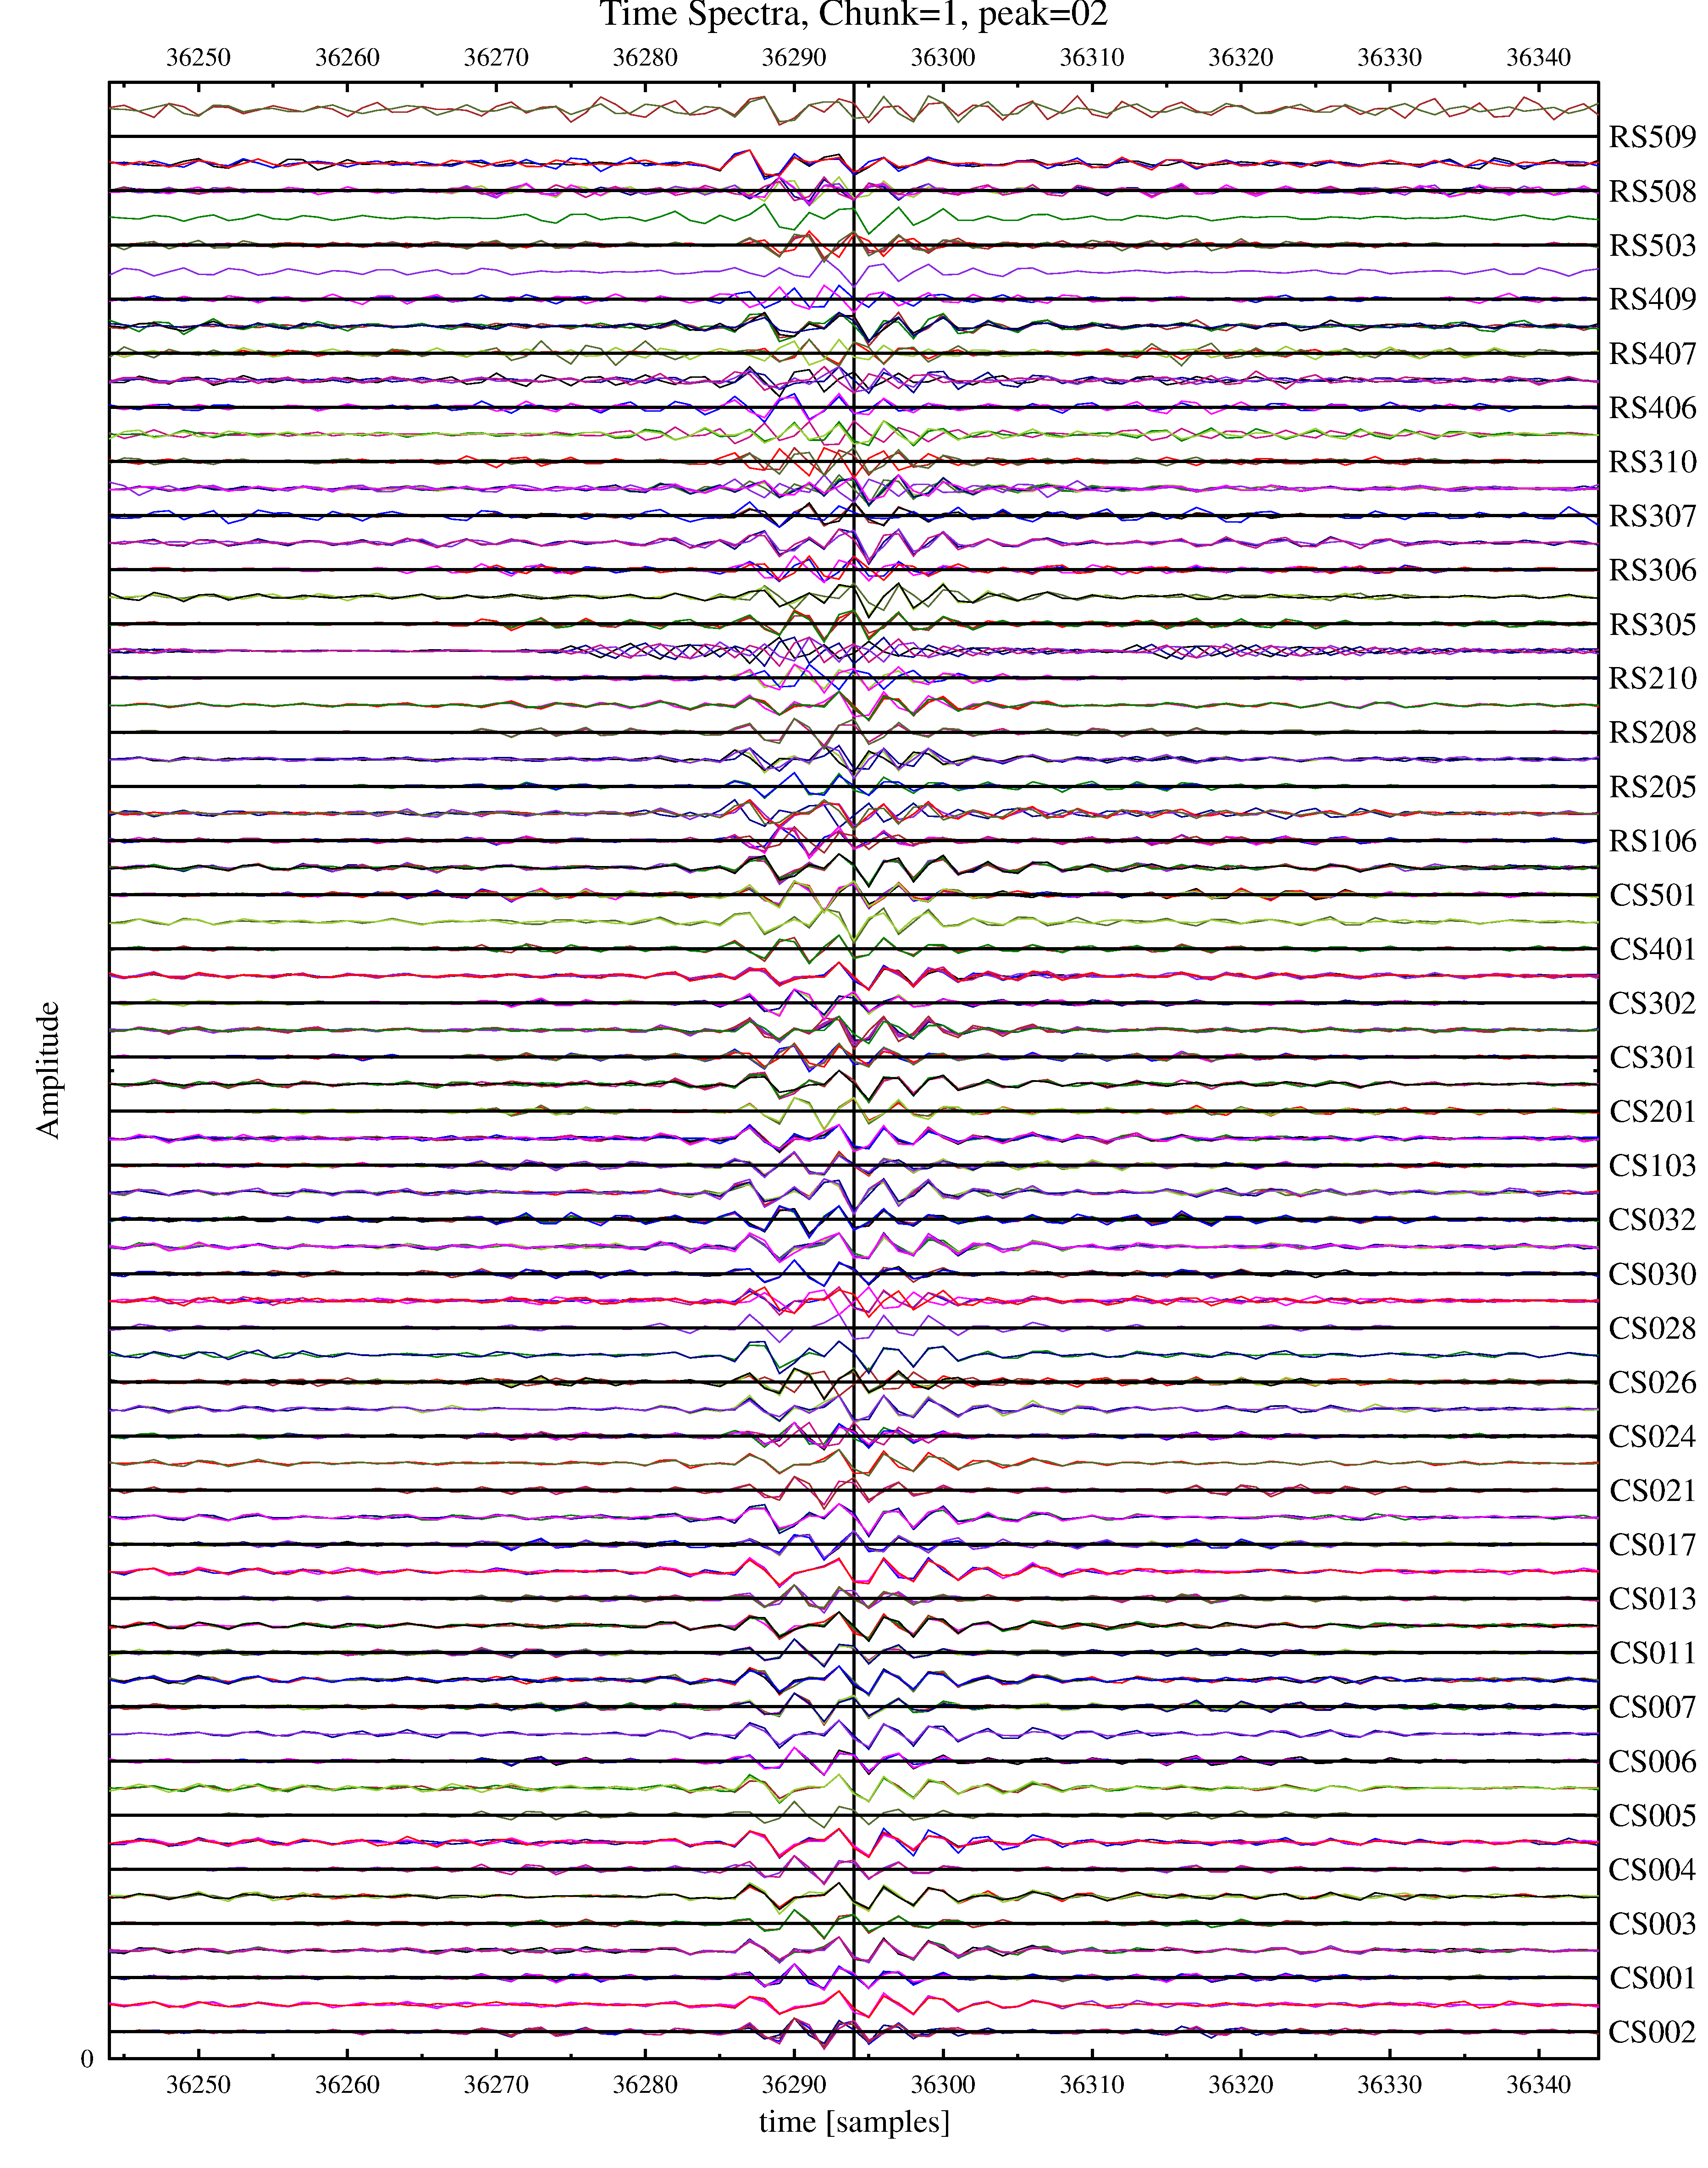
\includegraphics[width=0.59\textwidth]{Figs/CuP-02-18D1} }
%\centering{\includegraphics[ bb=1.0cm 2.4cm 24.5cm 25.7cm,clip, width=0.49\textwidth]{../Figs/SE20A7-NPMx_1HIntfSpecSel} }
	\caption{A curtain plot for the second source for a typical flash.}	 \figlab{Cal-Curtain}
\end{figure}

The pulses in all antennas can be included in the calibration calculation if the pulses line-up nicely. To see this better the time-window can be adjusted. The pulse amplitudes have been normalized for each spectrum to the maximum, say unity.
\\The structure of the pulses in all odd numbered antennas should resemble each other. The same for the even numbered antennas. The pulse for in the odd may be different from that in the even ones.
\\The noise level should hardly be visible on the plotted scale.
\\If one condition is not obeyed the antenna should be excluded for that particular source and that polarity of the antenna.

\subsubsection{Cross correlation plot}\seclab{XCorPlot}

\begin{figure}[th]
\centering{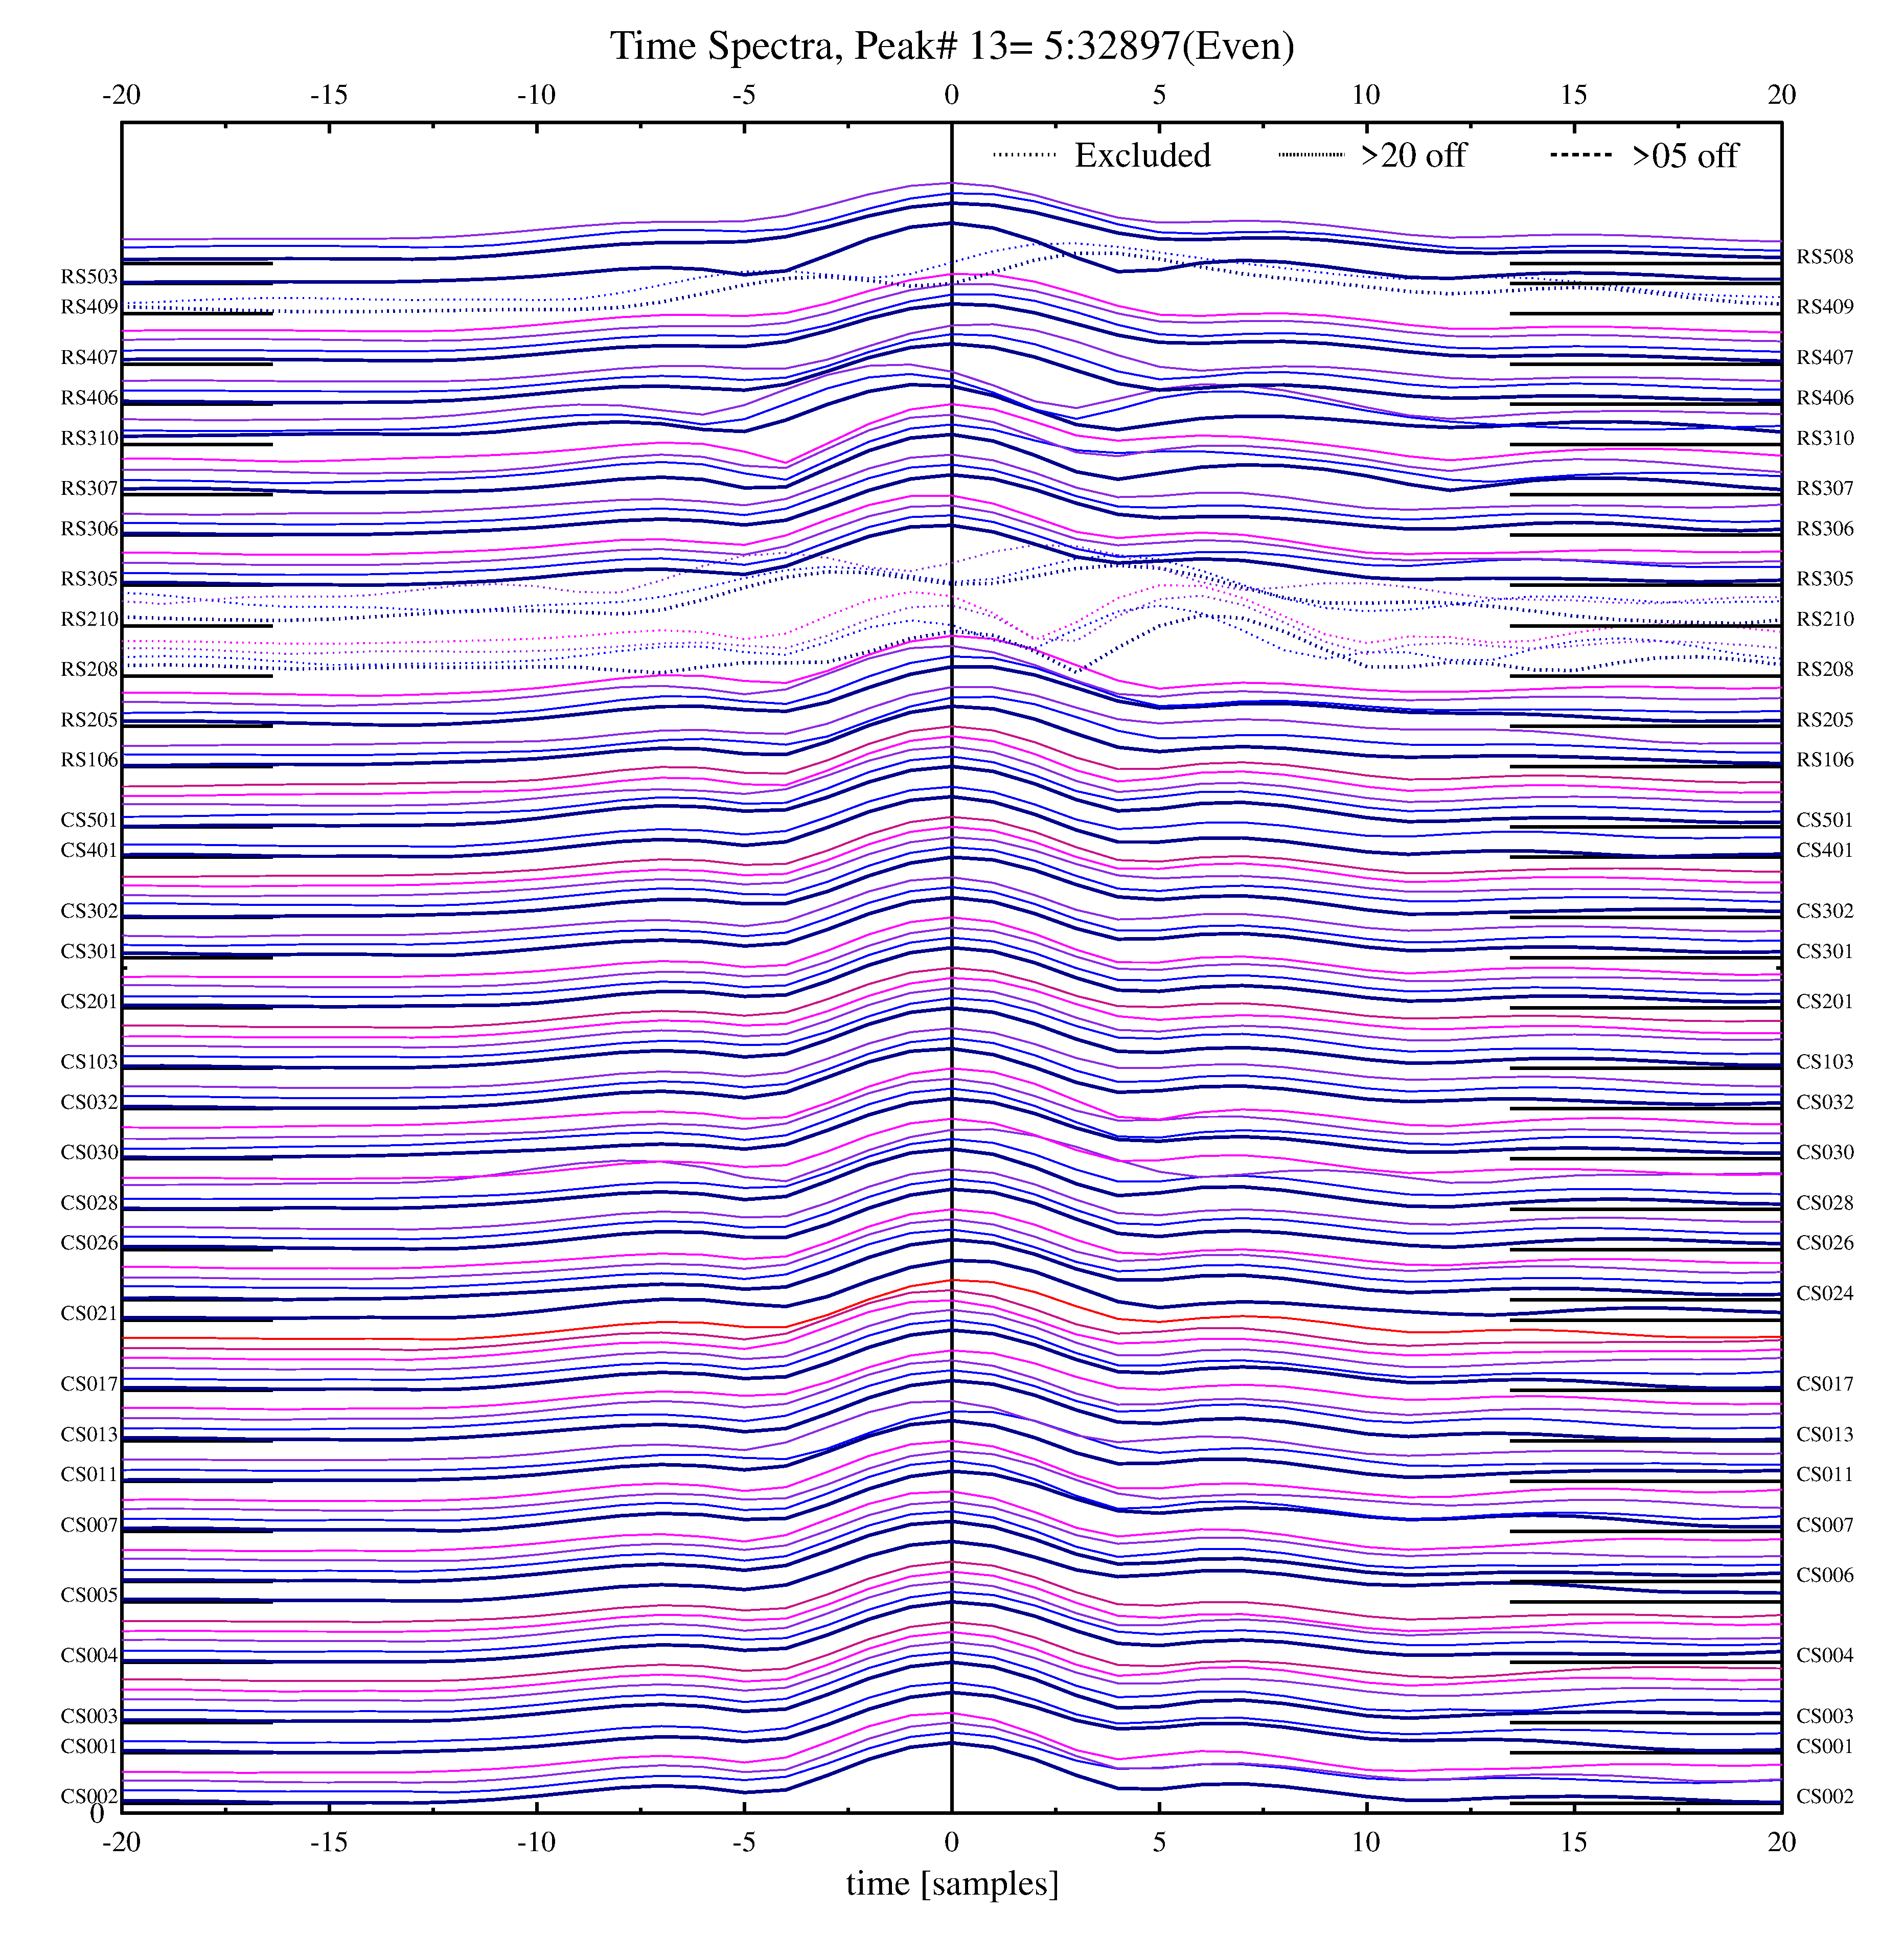
\includegraphics[width=0.69\textwidth]{Figs/XCP_13-18D1} }
%\centering{\includegraphics[ bb=1.0cm 2.4cm 24.5cm 25.7cm,clip, width=0.49\textwidth]{../Figs/SE20A7-NPMx_1HIntfSpecSel} }
	\caption{A plot of the absolute cross correlations for source \#13 for a typical flash.}	 \figlab{Cal-XCor}
\end{figure}

In \figref{Cal-XCor} a typical plot is shown of the cross correlations. The peak-time of these is used for calculating the arrival times differences that are fitted to obtain source positions. We usually work with the absolute magnitude as this yields better convergence than working with the real part. The real part has many oscillations which creates many local minima in a chi-square search, even though the position of the maximum can be determined more accurately. There is an option to plot the real parts.

For each antenna the Hilbert envelope is shown. The labels on the side helps to distinguish the different stations. Results are given in separate plots for even and odd numbered antennas. When all lines look alike, the result is good. Antennas, and stations should be excluded when the structure differs from that for the other antennas. The results for excluded stations is given by the dotted curves. It can be seen that for the case in \figref{Cal-XCor} most of them show a different structure. On the basis of these plots it may be decided to include a previously excluded station again in the fit. The paradigm is: the more the merrier, i.e.\ generally the results for the antenna calibrations are better if more stations are included, however, if for some of these station the pulse if unclear it could be that pulses from two different sources happen to arrive simultaneously in a particular antenna, the result improves if the -obviously- erroneous result is excluded. The art is to find the optimum between these conflicting requirements.


\clearpage
\subsubsection{Print output}\seclab{PrintOut}

Part a typical output (the .out file) that contains the most useful info for further processing is:

\begin{linenumbers}
\tiny
\resetlinenumber
\begin{verbatim}

i_Peak= 9 0, PeakPos=  16250, Chi^2/DegrF=   2.51   2.51, source position:   -2141.69,  -22721.36,    3935.67, RefAntTimeErr:  0.706
Stat Nr = CS001; CS002; CS003; CS004; CS005; CS006; CS007; CS011; CS013; CS017; CS021; CS024; CS026; CS028; CS030; CS032; CS103; RS106; CS201; RS208; RS210; CS301; CS302; RS305; RS306; RS307; RS310; CS401; RS406; RS407; RS409; CS501; RS503; RS508; -----
Dropped#=  0/ 5;  0/ 4;  0/ 4;  0/ 3;  0/ 2;  0/ 3;  0/ 4;  0/ 3;  0/ 6;  0/ 4;  0/ 2;  0/ 4;  0/ 5;  0/ 5;  0/ 4;  0/ 4;  0/ 5;  0/ 2;  0/ 4;  0/ 4;  0/ 3;  0/ 4;  0/ 5;  0/ 2;  0/ 3;  0/ 5;  0/ 4;  0/ 1;  0/ 1;  0/ 5;  0/ 1;  0/ 5;  0/ 4;  0/ 3; -----
RMS [ns]=   1.2;   0.6;   0.6;   0.8;   0.2;   0.4;   0.8;   1.0;   1.3;   0.7;   0.4;   0.5;   1.0;   0.9;   0.8;   0.5;   1.3;   0.9;   1.3;   2.4;   2.7;   0.4;   0.8;   0.6;   0.6;   3.5;   2.7;   0.5;   7.0;   2.6;   2.4;   0.5;   0.4;   2.3; -----
Avrg[ns]=   1.0;  -0.3;   0.5;   0.8;   0.1;  -0.3;   0.5;   1.0;   1.0;   0.5;   0.4;   0.3;   0.8;   0.4;   0.8;   0.3;   1.1;   0.5;   1.3;  -2.3;  -2.3;   0.3;   0.7;  -0.5;  -0.5;  -3.3;   2.0;   0.5;  -7.0;  -2.6;   2.4;   0.4;  -0.2;  -2.1; -----
RMS(Jac)=  0.06;  0.00;  0.02;  0.01;  0.02;  0.01;  0.01;  0.02;  0.05;  0.01;  0.05;  0.12;  0.02;  0.16;  0.13;  0.04;  0.04;  0.58;  0.05;  2.77;  4.06;  0.15;  0.21;  0.31;  0.56;  2.83;  6.46;  0.03;  2.10;  2.62;  6.03;  0.18;  0.51;  2.72;-----
\end{verbatim}
\end{linenumbers}

There is such a section for each peak. the ones towards the end of the output are for the last fits. This list for each station 1) the number of antennas that are dropped all together, because that one showed an unreasonably large difference; 2)the contribution to the RMS, 3) the mean time difference. If this matches (in absolute magnitude) the RMS for this station, then all antennas shaw about the same difference, if not, one of the antennas differs considerably. the last line shows the importance of this station for pinning down the source location.

Towards the end the following can be found

\begin{linenumbers}
\tiny
\resetlinenumber
\begin{verbatim}


C 6 1 2   18841 -72112.37,  21167.93,   5397.60,    0.00;   1.63,   1.67 RS406 RS509
exclude   RS406 RS509
C 7 0 3   27662  -6112.90, -28762.40,   6490.86,   -0.39;   1.80,   1.80
C 8 1 3   27662  -6112.90, -28762.40,   6490.86,   -0.37;   2.38,   2.50 RS208 RS210 RS310
exclude   RS208 RS210 RS310
C 9 0 4   16250  -2141.69, -22721.36,   3935.67,    0.71;   1.58,   1.58
\end{verbatim}
\end{linenumbers}

which follows the same formatting as the list needed in the input. With cut-and-paste it can thus be used conveniently. Per pulse it lists the fitted position and the value of the sqrt(chi-square) (last numbers) for this source. For a good result these numbers should not exceed 2 by much (units are nanoseconds). if the number is large, it should be searched which station is responsible for this, either by checking the listing for the pulse (see previous discussion) and/or checking the curtain and/or the cross correlation plots. This is the most tedious part of the calibration runs.

When the option \verb#" FullAntFitPrn=.true."# is switched on there is for each peak and each antenna, ordered per station, a list of the time differences between determined arrival times and calculated ones, i.e.\ the pull values for calculating the chi-square. On the basis of this information is may be decided to label a particular antenna as 'bad'. 
\clearpage
\section{Impulsive imaging}\seclab{Imag}

Source finding is performed by the script \verb!"Imaging.sh"! residing in the FlashFolder. The running of the script is controlled by \verb!"Imaging.in"!, which typically resembles


\begin{linenumbers}
\resetlinenumber
\begin{verbatim}
&Parameters
 RunOption='Impulsive'
   Dual=.false.  ! Fix pulses in the even (Y-) and odd (X-) numbered dipoles at same source position.
! ChiSq_lim= 80 ! max value for chi^2 of a source for it to be stored (RMS=sqrt(chi^2)
! NoiseLevel=80. !  Any weaker sources will not be imaged.
! AntennaRange=100	! maximal distance of antennas to the reference antenna [km]
! PeaksPerChunk=500 !  Maximum number of sources searched for per chunk (of 0.3 ms).
! CalibratedOnly=.true. !  Use only antennas that have been calibrated.
! FullSourceSearch=.true. !  Perform without any preferred direction, otherwise take the sourceguess as a preference.
! Simulation=" " !  Run on simulated data from such files.
! EffAntNr_lim=0.8 !  minimal fraction of the total number of antennas for which the pulse is located.
! CCShapeCut_lim=0.6 !  Maximum ratio of the width of the cross correlation function by that of the self correlation.
! SearchRangeFallOff=4. !  Multiplier for the (parabolic) width of the pulse-search window.
! Sigma_AntT=3 !  Constant added to width of search window for pulses.
 Calibrations= "Calibrations201912042045.dat"
 BadAnt_SAI=   003065, 021078, 021079, 021093, 026030, 32016, 32017, 32048, 32049
               101045, 125029, 150065, 188051, 188094, 188095
 OutFileLabel="-s"
&end

C  1165 , -45500.  7700.   5300.0 , 101.7 300  !  StartTime_ms , (N,E,h), t_init [ms], t_fin [ms] (after start)
\end{verbatim}
\end{linenumbers}

While in imaging mode only very few parameters need to be specified and often the default settings will suffice.
\begin{enumerate*}
\item[2] \verb#"RunOption='Impulsive'"#: Run in impulsive imaging mode.
\item[3] \verb!" Dual=.false."!: The peaks in even and odd numbered antennas will be searched for independently.  \\
    \verb!" Dual=.true."!: In searching for the source locations the peak positions in both even- and odd-numbered antennas are used.
\item[4] \verb#"! ChiSq_lim= 80."#: Sources with a chi-square better than 80 will be stored.
\item[5] \verb#"! NoiseLevel = 80."#: The source location will be searched only for pulses with an amplitude in the reference antenna greater than 80.
\item[6] \verb#"! AntennaRange=100"#: All antennas within a distance of 100~km (the max possible) will from the reference antenna will be included in the calculations.
\item[7] \verb#"! PeaksPerChunk=500"#; Maximum number of sources searched for per chunk (of 0.3 ms).
\item[8] \verb#'! CalibratedOnly=.true.'#: Only antennas used in the calibration run will be used for imaging.
\item[9] \verb#"! FullSourceSearch=.true."#: Perform without any preferred direction, otherwise take the sourceguess as a preference.
\item[10] \verb#'! Simulation=" " '#: Run on simulated data from thus named files files, see \secref{?}.
\item[11] \verb#"! EffAntNr_lim=0.8" #:  minimal fraction of the total number of antennas for which the pulse is located.
\item[12] \verb#'! CCShapeCut_lim=0.6 '#:  Maximum ratio of the width of the cross correlation function by that of the self correlation.
\item[13] \verb#"! SearchRangeFallOff=4. " #:  Multiplier for the (parabolic) width of the pulse-search window.
\item[14] \verb#"! Sigma_AntT=3 " #:  Constant added to width of search window for pulses.

\item[15] \verb!' Calibrations = "Calibrations201912042045.dat"'!: The name of the calibration file created at the end of the time calibration procedure.
\item[16] \verb#" BadAnt_SAI=   003065, "#: The antenna SAI identifiers (see \secref{RFI-out}) of the antennas that do not have good data.
\item[18] \verb#' OutFileLabel="-s" '#: An additional label for the output files, including the list of sources.
\item[21] \verb#"C  1165 , -45500.  7700.   5300.0 , 101.7 300 "#: Specification of the starting time, approximate location of the flash, and the time frame where sources should be searched. If `S' is used instead of `C' (or space) the given time will correspond to the time at the indicated position.
\end{enumerate*}
The last line in the input specifies
\\1) The start time, $T_0=1165$  (in ms), of the flash. The output of the RFI-mitigation and also that of the Explore runs should give you a reasonable estimate of when the flash started.
\\2--4) The general direction towards the flash (N,E,h) in m.
\\5) The time after $T_0$ (in ms) to proceed with source finding. It may be negative.
\\6) The time after $T_0$ (in ms) to stop with source finding.

\subsection{details}

The results for the source locations are written to \verb!Srcs18-dblxxxx.csv! or otherwise the files \verb!Srcs18-oddxxxx.csv! and \verb!Srcs18-evenxxxx.csv! in the FlashFolder.
These .csv files are plain text files and contain some header lines with some general information followed by the specific data of the sources that are found and pass some very crude criteria. In particular $\chi^2<$\verb!ChiSq_lim!. The data for the sources is organized in columns where:
\\col1: Unique label composed from the chuck number (after $T_0$) and the pulse number in the chunk.
\\col2-4: distances northward, eastward, upward [m].
\\col5: Time at the source [s].
\\col6: $\chi^2$, if this had units, they would be [ns$^2$] .
\\col7-9: 1 std error in north, east, vertical direction [m].
\\col10: Number of antennas that have contributed to imaging this source.
\\col11: Total number of antennas for which data are available for this chunk.

See later sections for the details of the source-finding procedure including the criteria for excluding antennas.

\subsection{output}

The most important output is the list of source locations with their quality identifiers. Additionally a plot is made of the peak-finding statistics like shown in \figref{PeakStat}.

\begin{figure}[th]
\centering{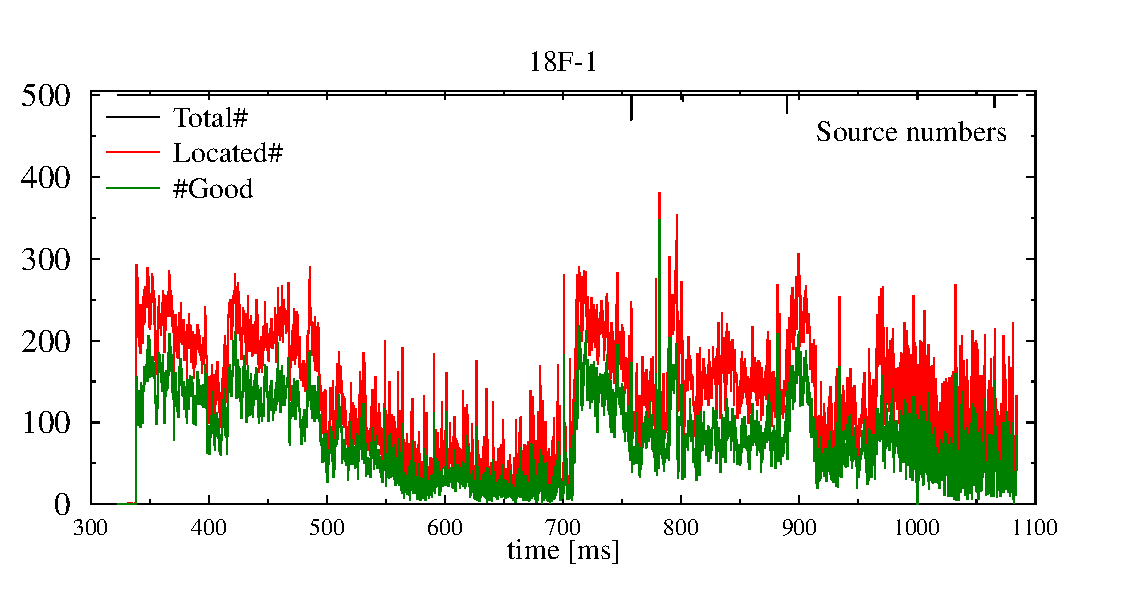
\includegraphics[bb=0cm 0cm 25.5cm 31.4cm,clip, width=0.49\textwidth]{Figs/PeakStats} }
%\centering{\includegraphics[ bb=1.0cm 2.4cm 24.5cm 25.7cm,clip, width=0.49\textwidth]{../Figs/SE20A7-NPMx_1HIntfSpecSel} }
	\caption{Statistics of the source-finding procedure for the impulsive imager. For each time frame the number of located sources is given with a chi-square below the maximum specified.}	 \figlab{PeakStat}
\end{figure}

\section{Plotting flashes}

For plotting it is advised to use the script \verb!FlashImage.sh! that reads the input from \verb!FlashImage.in! specifying values for the quality indicators as well as the windows for which the source locations and timings will be plotted. The script \verb!FlashImage.bat! is for running under windows.

\begin{linenumbers}
\resetlinenumber
\begin{verbatim}
 "Srcs18-evenS" 5. 2. 3.0 55   18D1e-i   -30.00 -27.  -7.5 -5.0  4.5 7.0  0. 30.  NoBox
 0.1 0.5 0.1      ""  1.  1.   1   0.5                                             ! MaxTrackDist[km], Wtr[0.5], TimeWin[ms^2]
======================================================
\end{verbatim}
\end{linenumbers}

The first line gives in order:
\\1) The name of the .csv file containing the sources data as created by an imaging run.
\\2) The cut $ \sigma_0^h $ on $\sigma{h}$
\\3) The height $h_0$. All sources higher than $h_0$ are plotted when  $\sigma{h} < \sigma_0^h$. Sources at lower altitudes $h$ will be plotted when $\sigma{h} < \sigma_0^h \times (h_0/h) $.
\\4) RMS cut value, in [ns].
\\5) $N_{ex}$, the maximum number of excluded stations.
\\6) naming of the .pdf file containing the image.
\\7 -- 14) limiting values for east, north, height (all in [km]) and time (in [ms] after $t_0$
\\15) if "NoBox" is specified, no high-lighting box will be drawn, otherwise the coordinates of the box will be read from the files for the specified plot.

The second line gives the parameters for calculating track that will be indicated in the image of the sources. In order:
\\1) maximal distance for a source to be removed from the track-head to be assigned to a track.
\\2) Weighting of additional points to determine the position of the track-head.
\\3) Width of gaussian time window to smooth the track.
\\4) Name of file containing predefined track.
\\5) Binning window for determining track statistics such as velocity.
\\6) Factor to scale height in the calculation of relative distances.
\\7) Integer. The maximum number of tracks to be generated.
\\8) Factor used to scale intensity-dependence of the size of the dots when plotting source positions.

\begin{figure}[th]
\centering{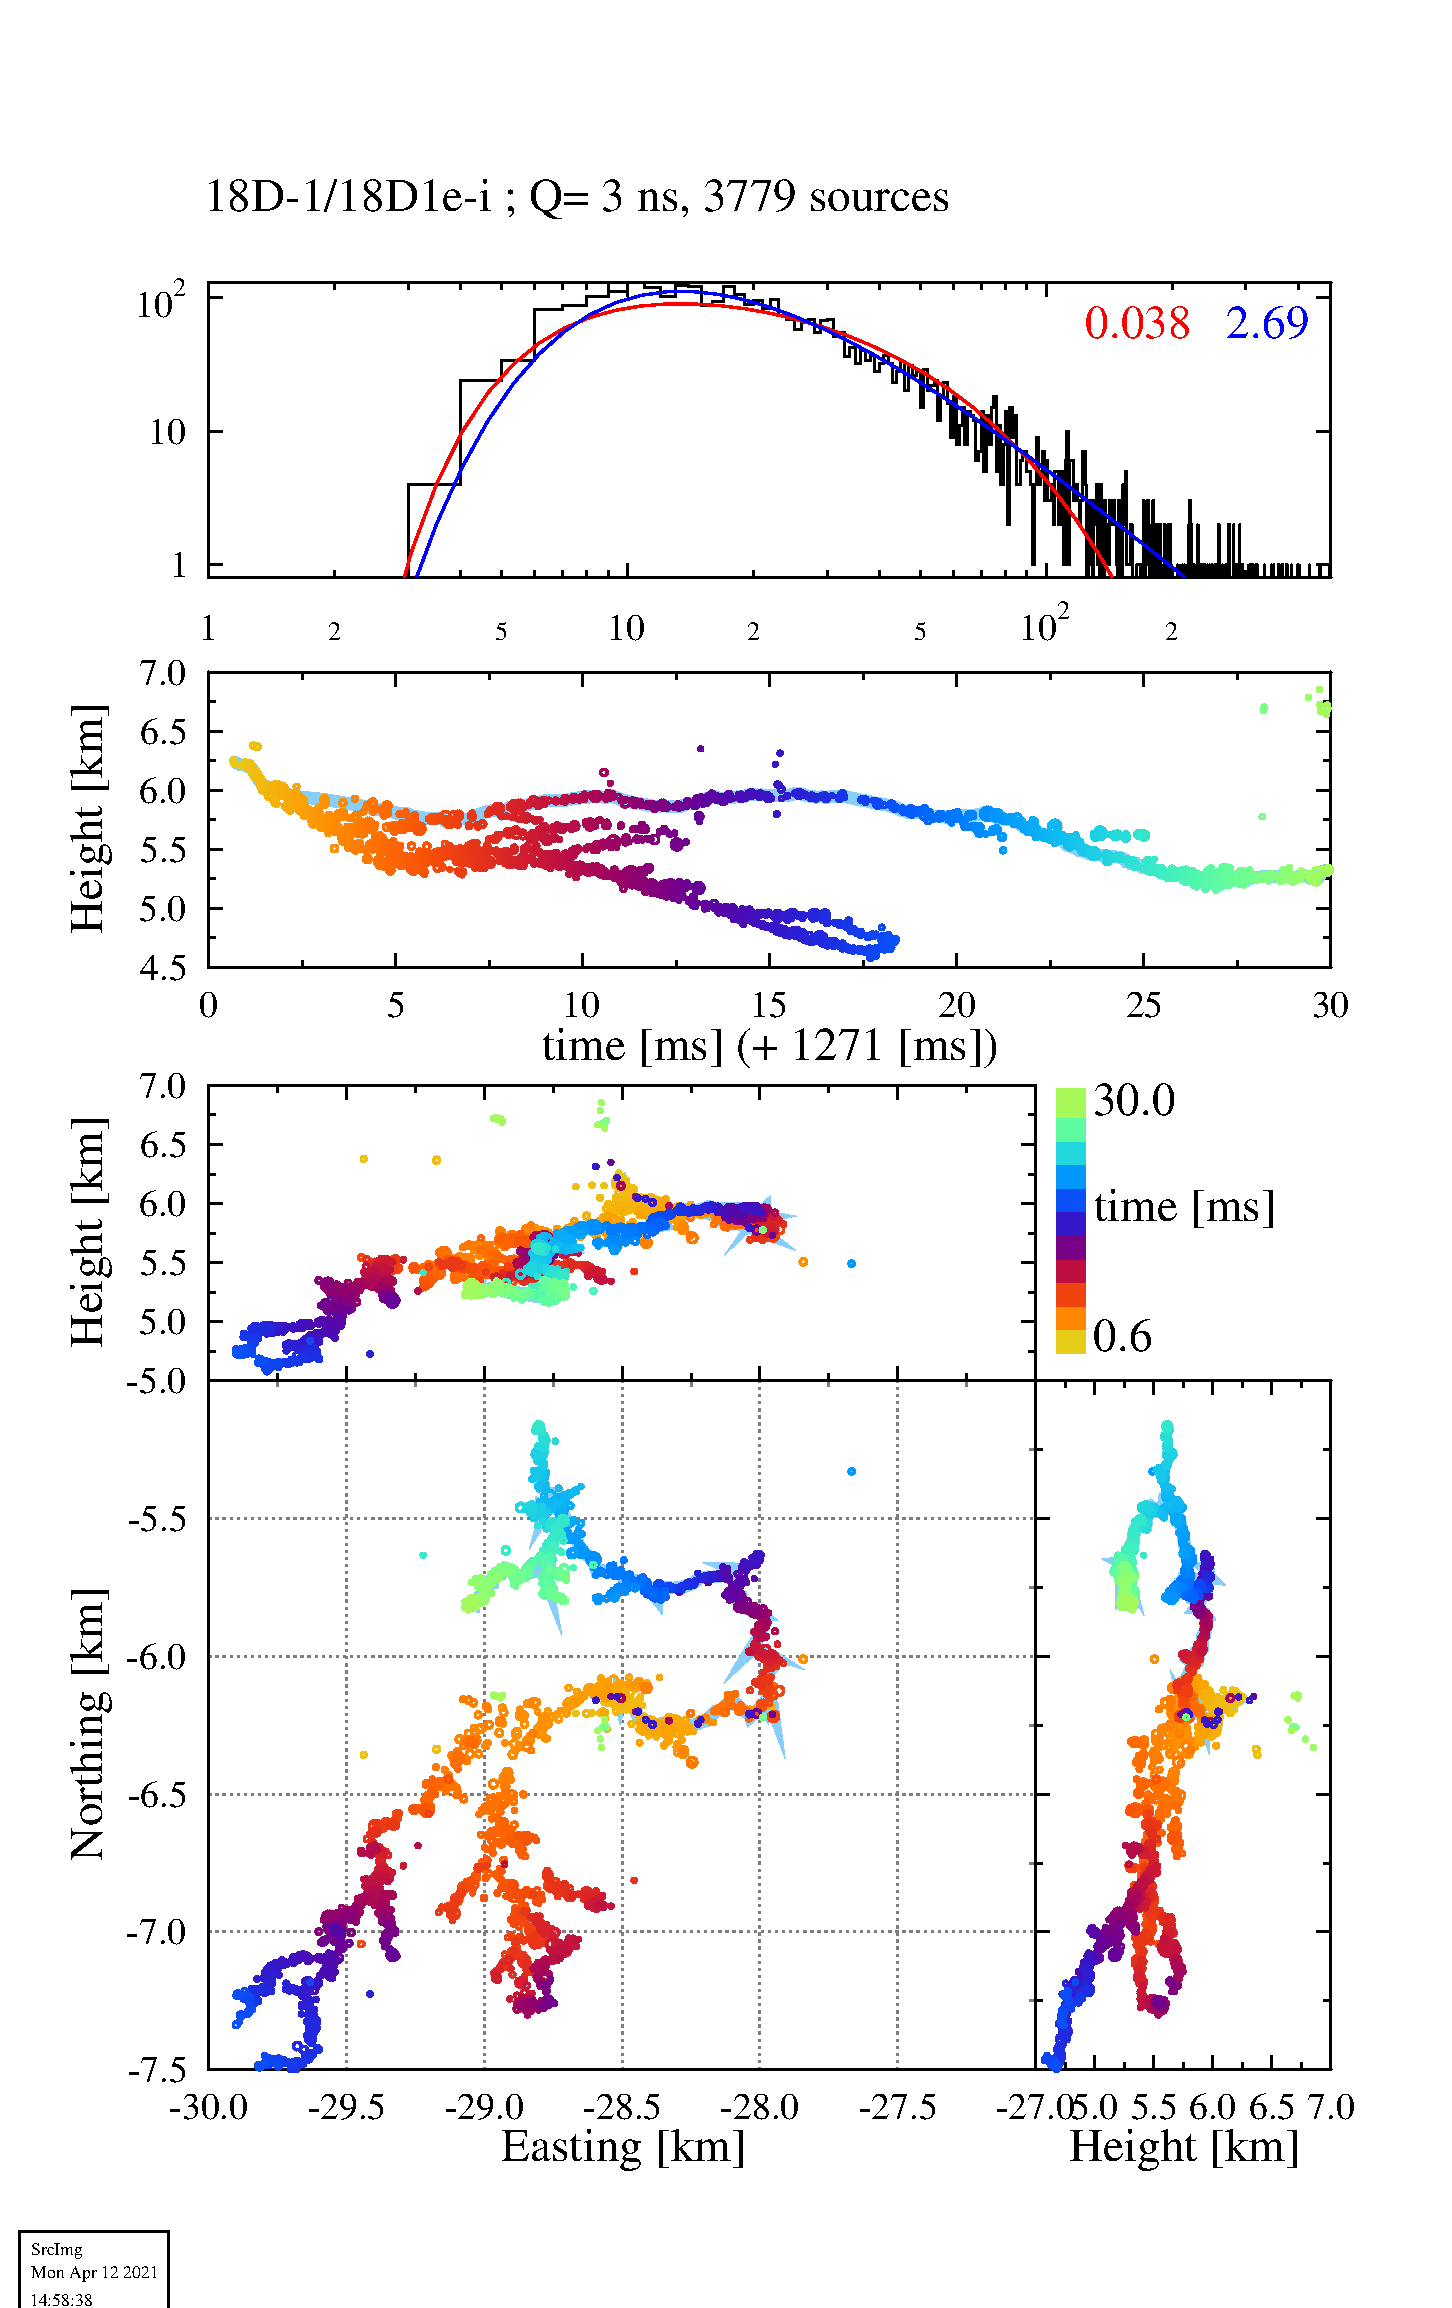
\includegraphics[width=0.49\textwidth]{Figs/Imp_18D1e-i} }
%\centering{\includegraphics[ bb=1.0cm 2.4cm 24.5cm 25.7cm,clip, width=0.49\textwidth]{../Figs/SE20A7-NPMx_1HIntfSpecSel} }
	\caption{Typical image for the Impulsive Imager as created by running ``FlashImage.bat". Light blue band is the reconstructed track (starting from the latest point and tracing back). Top panel give pulse power statistics where the modified exponential is plotted in red and the modified power law plotted in blue.}	 \figlab{ImpulsiveImg}
\end{figure}

The result is displayed in \figref{ImpulsiveImg} for the image of the flash for the selected area. The normalized pulse powers distributions $N(I)$ are fitted with a modified exponential,
\begin{equation}
N(I)= {\cal N}_e \,e^{-\alpha_e\,I-\gamma_e/I^2}\;, \eqlab{PowLaw}
\end{equation}
as well as with a modified powerlaw,
T\begin{equation}
N(I)= {\cal N} \,I^{-\alpha}  \,e^{-\gamma/I}\;, \eqlab{PowLaw}
\end{equation}
where $I$ is expressed in units of [GB]. The last factor, dependent on $\gamma$, suppresses the distribution at small amplitudes to good agreement with the data. The values for the fitted values for the normalization ${\cal N}$, the power $\alpha$, and the small-intensity suppression factor $\gamma$ are given in the output file (with extension .out).

\begin{figure}[th]
\centering{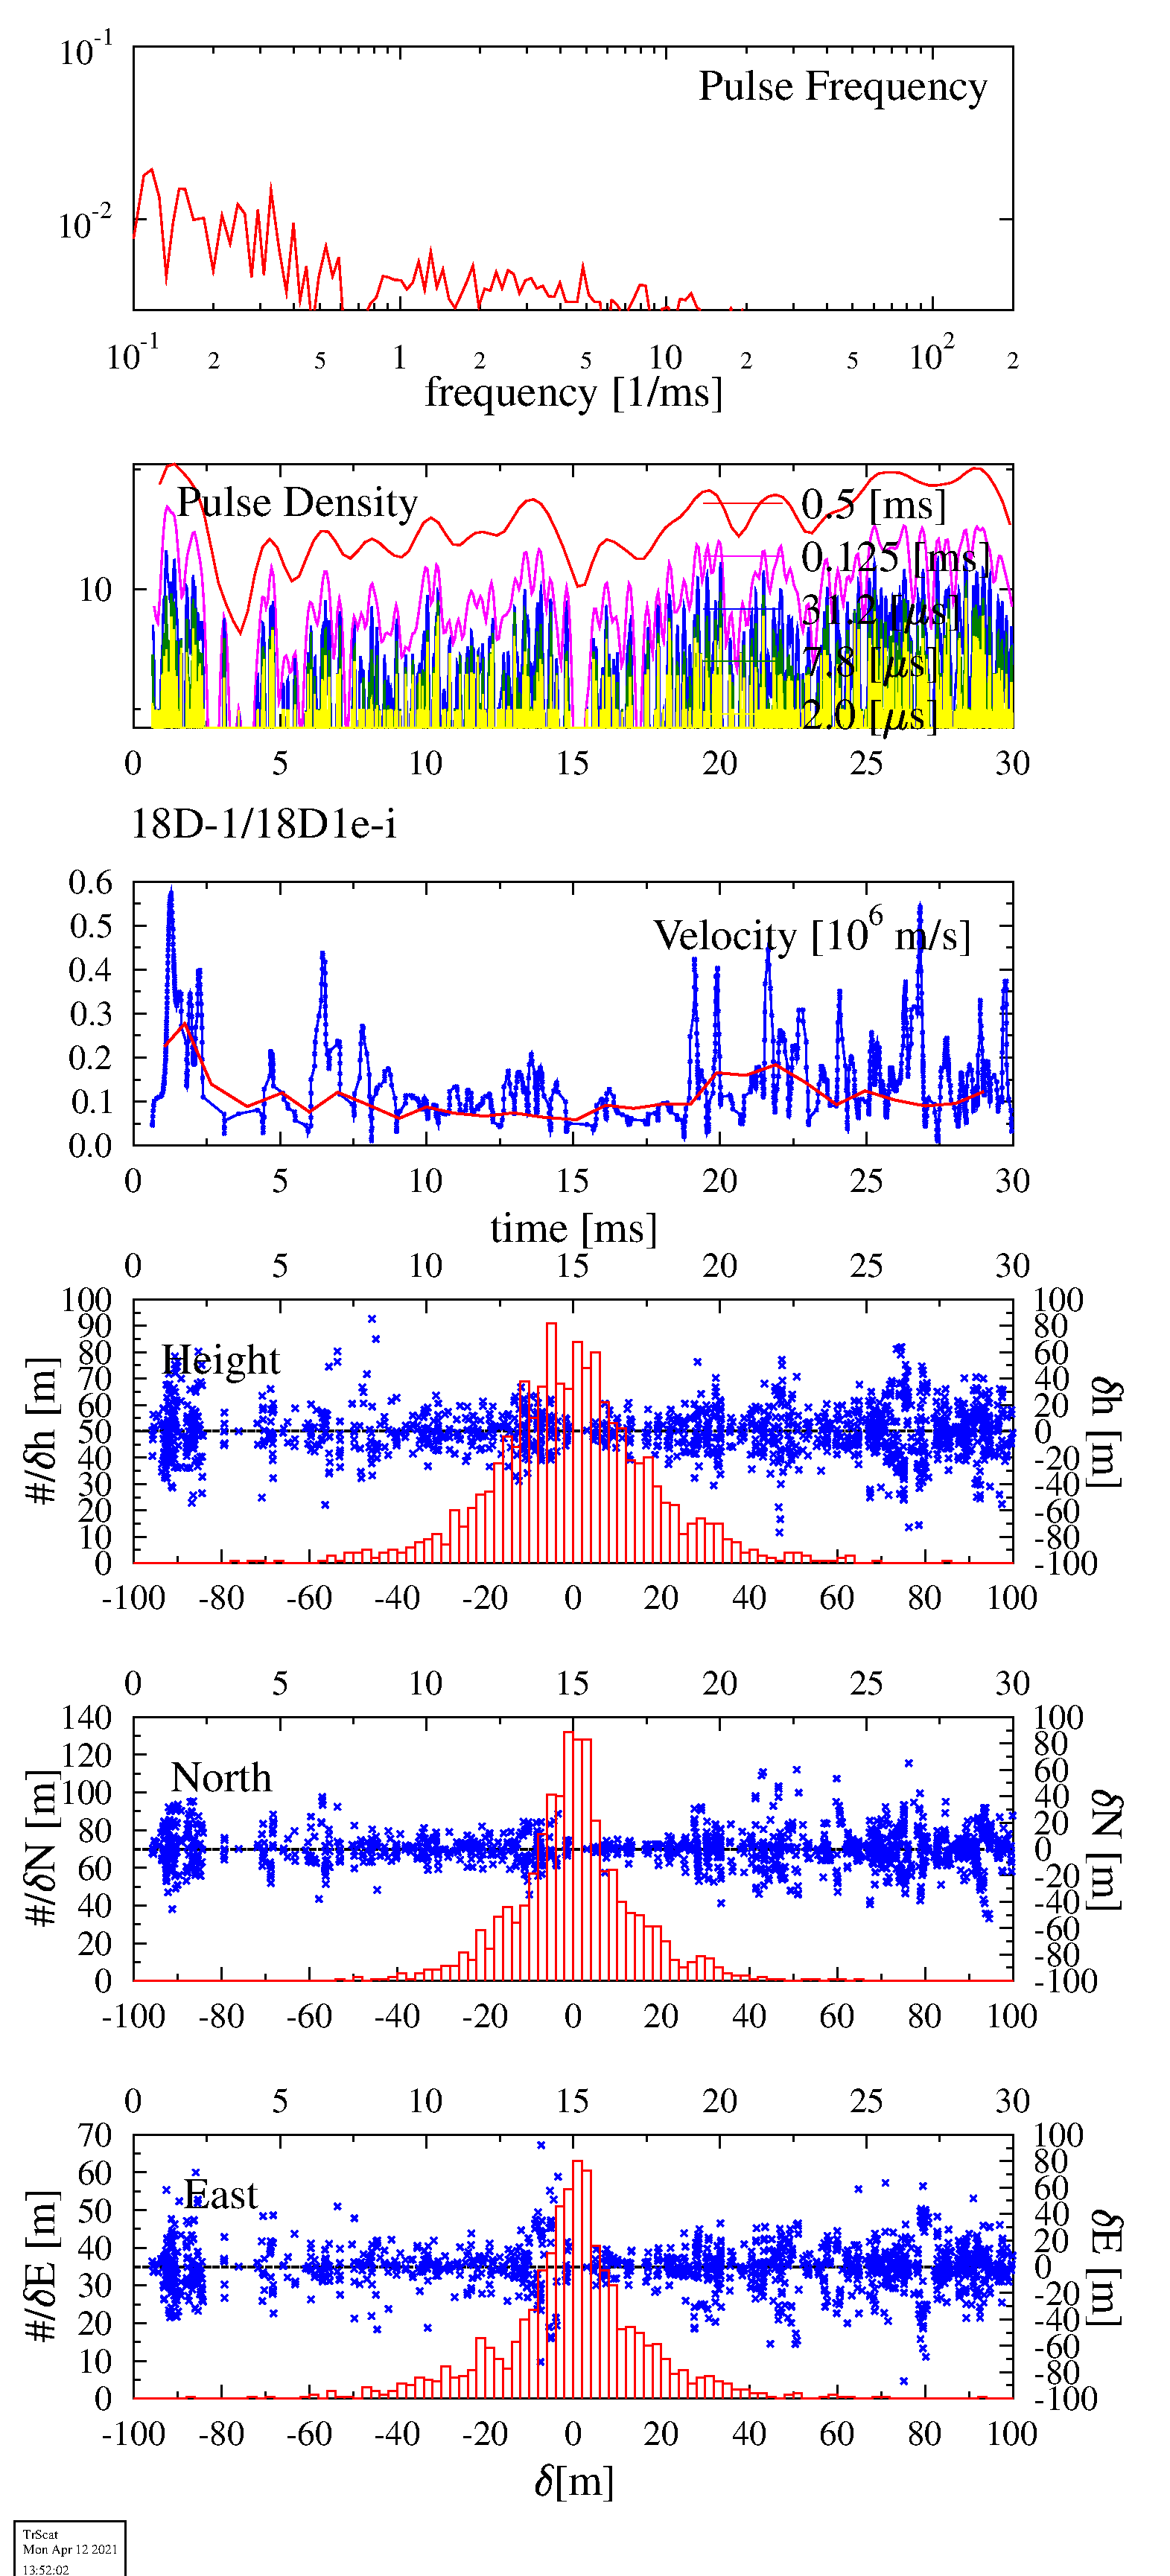
\includegraphics[ width=0.49\textwidth]{Figs/TrSc_18D1e-i} }
%\centering{\includegraphics[ bb=1.0cm 2.4cm 24.5cm 25.7cm,clip, width=0.49\textwidth]{../Figs/SE20A7-NPMx_1HIntfSpecSel} }
	\caption{Typical image for the Impulsive Imager when showing the statistics along a track.}	 \figlab{ImpulsiveTrack}
\end{figure}

If the 7th number on the second line in the input, ``FlashImage.in", is positive, a graph like \figref{ImpulsiveTrack} is made for each track. The second panel from the top shows the pulse density along the flash as function of time for various width of a gaussian smoothing function. The top panel shows the fourier decomposition of this plot. The third from the top gives the velocity along the track. The blue line for each source along the track, the red line for an average leader-tip location. The bottom three panels show the spread of the sources in the three directions from the propagating tip of the leader, in blue as a scatter plot v.s.\ time of the source (top and right scales), in red as a histogram (bottom and left scales).
\clearpage 
\section{TRI-D Interferometric imaging}\seclab{Intf}

Interferometry can be performed working only with the signals measured in the antennas, i.e.\ without unfolding the antenna function, and is referred to as Signal Interferometry (SI), which is by now considered obsolete. This because the method has many unsolved issues with signs due to the antenna function and the emission pattern being angle dependent. More sophisticated is to convert the measured signal in the X- and Y- dipoles to the radiation electric field at the antenna and use this for interferometry, presently the preferred and only option. This will be named E-field Interferometry (EI) when it needs to be contrasted with SI.

Source finding is performed by the script \verb!"Interferometry.sh"! residing in the FlashFolder. The running of the script is controlled by \verb!"Interferometry.in"!, which typically resembles:

\begin{linenumbers}
\resetlinenumber
\tiny
\begin{verbatim}
 &Parameters  RunOption= "TRI-D"
 OutFileLabel= "XYZ"
 AntennaRange= 100.     ! Maximum distance (from the core) for the range of the antennas (in [km]).
 TimeBase=320.    ! Time-offset from the start of the data, best if kept the same for all analyses for this flash
! Simulation= ""     ! Run on simulated data from such files.
! ChainRun= 0     ! Automatically start jobs (for - previous or + following timeslots, made to follow a negative leader.
! IntfSmoothWin= 19     ! Width (in samples) of the slices for TRI-D imaging.
! PixPowOpt= 0     ! =0=default: Intensity=sum two transverse polarizations only; =1: Intensity=sum all polarizations weighted with alpha == intensity of F vector; =2: Intensity=sum all three polarizations, including longitudinal with the full weight
! CalibratedOnly= T     ! Use only antennas that have been calibrated.
 NoiseLevel= 1.0000000000000000E-002     ! Any weaker sources will not be imaged.
 Calibrations="Calibrations202202071332.dat" ! FldCal all antennas
 BadAnt_SAI=   5095,   7093,  11089,  13088,  13089,  17084,  17085,  17094,  17095
               101085, 141083, 141086, 141087, 167094, 169082, 169090, 169094,
 ExcludedStat=  "RS305"      ! Mnemonics of the stations that should be excluded.
 SignFlp_SAI=  142092, 142093
 SaturatedSamplesMax= 3     ! Maximum number of saturates time-samples per chunk of data
 &end  !
S  231.  8.2 ,-3.7, -34.11    !    Reference/Source-| time, & position
C   80 2.5, 30 2.5, 72 4 !   Polar(Phi,Th,R)/Carthesian(N,E,h) | 3x(#gridpoints, grid spacing)
F  25000  15000 10.   !  First/Median| SumStrt, SumWindw, AmpltPlot
\end{verbatim}
\end{linenumbers}

The lines in the namelist \verb!"&Parameters"! input specify:
\begin{enumerate*}
\item \verb!RunOption= "TRI-D"!: Run the TRI-D Imager
\item \verb!OutFileLabel="XYZ"!: Additional label used for the output files, including the plots.
\item \verb!AntennaRange=100.!: The maximal distance (in [km]) from the reference station of the antenna stations that are included in imaging.
\item \verb!TimeBase=320.!: This time is added to the relative time specified in the input.
\item \verb# Simulation= ""#: No simulated data are used in blank, otherwise the simulated data are read from these files and should have the same value as used when generating the simulated data, see \secref{Sim}.
\item \verb# ChainRun=0# (Integer, default=0): If =0 the present run will not spawn any children, otherwise see \secref{ChainRun}.
\item \verb!IntfSmoothWin=19! (Integer, default=20): the width of the sampling function used for Time Resolved Imaging (in [samples]). This number should be of the order of the impulse-response time, about 20~samples.
\item \verb!PixPowOpt=! (Integer, 0): selects how the intensity of a pixel is calcula
   \\\verb!PixPowOpt =0! (default): sum two transverse (as seen from the core) polarizations only.
   \\\verb!PixPowOpt =1! : sum all polarizations weighted with alpha to compensate $A^{-1}$ thus intensity =  $|\vec{F}|$, see \eqref{F_as}.
   \\\verb!PixPowOpt =2! : Sum all three polarizations, thus including longitudinal with the full weight.
\item \verb!CalibratedOnly= T! (logical, .true.): use only antennas that have been calibrated.
\item \verb!NoiseLevel=!: only sources with a coherent intensity exceeding this value will be imaged.
\item \verb!Calibrations =""!: The name of the file containing calibration data.
\item \verb!"BadAnt_SAI="!: These antennas are excluded from the analysis.
\item \verb!"SignFlp_SAI="!: The amplitude for this antenna is multiplied by minus unity.
\item \verb!"ExcludedStat="!: Mnemonics of the stations that will be excluded from interferometry. The exclusion is usually based on unexpected phases.
\end{enumerate*}


The following lines specify:
\begin{enumerate*}
\item[line +1:]   ``\verb#S  231.  8.2 ,-3.7, -34.11#''
   \begin{enumerate*}
   \item[1] Option, "R" or "S" (capital, the very first character on this line): time is specified at the Reference antenna or at the Source location for the tesseract.
   \item[2] $t_t$, the starting time of the data-chunk in which the tesseract is taken, given in time [ms]. Time is taken relative to \verb!"TimeBase"!.
   \item[3-5] Space coordinates of the center of this tesseract, in (N,E,h) notation. The units may be [km] or in [m], but have to be the same for all three.
   \end{enumerate*}
\item[line +2:]   ``\verb#C   80 2.5, 30 2.5, 72 4#''
   \begin{enumerate}
   \item[1] Option, "P" or "C" (capital, the very first character on this line): determines if a Polar or Cartesian grid is used for the tesseract. The polar grid is taken as a wedge, focussed ar the reference antenna. A Polar grid is specified in the order: Azimuth angle $\phi$, elevation angle $\theta_e$, and distance to reference antenna $R$. A Cartesian grid as: Northing $N$, Easting $E$, and altitude $h$.
   \item[2, 4, 6] Number of grid points, counting from the center.
   \item[3, 5, 7] Grid spacing in degrees or meter.
   \end{enumerate}
   or
   \begin{enumerate}
   \item[1] Option, "Q" or "D" (capital, the very first character on this line): determines if a Polar or Cartesian grid is used for the tesseract. The polar grid is taken as a wedge, focussed ar the reference antenna. A Polar grid is specified in the order: Azimuth angle $\phi$, elevation angle $\theta_e$, and distance to reference antenna $R$. A Cartesian grid as: Northing $N$, Easting $E$, and altitude $h$.
   \item[2] Fineness coefficient.
   \item[3, 4, 5] Box size in 3D.
   \end{enumerate}
\item[line +3]:   ``\verb#F  25000  15000 10.#''
   \item[1] Option, ``F" or ``M" (capital, the very first character on this line): determines if the time is set at the First or the Middle sample of the time window.
   \item[2] (integer): Time-offset of the tesseract from the start of the data chunk, in samples of 5 ns. Care should be taken that the start of the tesseract is at least 1000 samples from the beginning of the data chunk to avoid antennas from dropping out. Error messages are generated and image is truncated when the value is too small. If option ``F" (``M") is specified the value is pointing to the First (Middle) time sample of tesseract.
   \item[3] (integer): The length of the window (in [samples]) that is imaged. The maximum window length is 60k~samples (corresponding to 0.3~ms) to which 40 (=$2\times$"IntfSmoothWin") may be added is to accommodate for the beginning and end smoothing windows when performing Time Resolved Imaging (see \secref{TRID}).
   \item[4] : an indicator of the maximum size of the circles used in plotting, taken proportional to source intensity. If negative, dots are used and the intensity spectrum is not analyzed.
\end{enumerate*}


This script produces TRI-D images (see \secref{TRID} for the procedures followed)
and puts the results in several data files in the subdirectory \verb!"files"!. It also prepares the commands in a file with name starting with ( \verb!"Afig-Intf"!) for running the GLE scripts \cite{GLE} to produce the plots discussed in \secref{Interf}.

It is recommended to subsequently run the script \verb!"DataSelect.sh"! using \verb!"DataSelect.in"! as input to produce the plots that are zoomed in on the region of interest, see \secref{DataSelect}

\subsection{Chainrun} \seclab{ChainRun}

If \verb# ChainRun=0# the present run will not spawn any children, otherwise, a chain of jobs will be generated to allow for the TRI-D imager to follow the track of a leader, or to image a fixed spot for a long time period.
if \verb# ChainRun=0# is non zero line ``+1'' may have a different structure which is determining what the structure of the chaining will be.

Typically [line +1] may read:  ``\verb#S  825.15   "I-19A-1b-D3a.trc" #'' where the space coordinates have been replaced by a file name containing a track. The first few lines of this file could read
{\tiny
\begin{verbatim}
   825.0   -12.  -27.05   7.6
   826.12   -12.  -27.05   7.6
  826.12049     -11.872760     -26.808671      7.4762350
  826.13483     -11.822525     -26.901188      7.5054529
  826.14391     -11.817934     -26.985353      7.4927362
\end{verbatim}
}
where the bulk of the file was generated using the 'longtrack' option in utility \verb!DataSelect! as described in \secref{DataSelect}. Each line gives the coordinates of the track as (time, N, E, h). The file may also be a .dat file (in stead of .trc),  having the same format at image-source files, i.e.\ (label, t, x, y, z). The program will construct a cube of size as specified in [line +2] centered at the the position on the track at time $t_t$=825.15 for the present example. At the end of the run an input for a following job is created where the time on the track is increased by the time duration of the tesseract. \verb# ChainRun# will be decreased by one and a new job is submitted. This proceeds till \verb# ChainRun# is reduced to zero, or the end of the track is reached. The present value of \verb!"ChainRun"! is worked into \verb!"OutFileLabel"! as well as the naming of the spawned scripts.

When \verb# ChainRun# is negative, the time of the next run will be decreased and \verb# ChainRun# is increased, i.e.\ the track is scanned in the opposite direction as before.

In case not a track, but coordinates are given, the program will center the new image cube at the center of intensity of the present image. This option sounds fancy but in practice does not really perform up to expectation.

If the track file name is followed by a positive real, this is interpreted at the time on the track. The tesseracts will follow the track in space coordinates, but are all taken at the same fixed time given by $t_t$. The next image box is now taken such that the side touches that of the previous, independent of the time duration of the tesseract, but following the track. This option is used in Ref.~\cite{Scholten:2023PL}.

\subsection{Output}\seclab{Interf}

The produced .dat files are plain text files and contain some header lines with some general information followed by the specific data of the sources that are found and pass some very crude criteria. The files have a format that is suitable for the plotting script \verb!"SourcesPlot.gle"!. The naming of these data files is as in \verb!"XYZIntfSpecPowMx_d.dat"!, where \verb!"XYZ"! is set by the user through \verb!"OutFileLabel=XYZ"! when running the interferometry option; \verb!"IntfSpecPow"! is fixed for these kind of files; \verb!"Mx"! implies that these source positions were determined using the quadratic maximum search while for \verb!"Bar"! the, by now obsolete, barycentric procedure was used, see \secref{Max}.
This file also contains the coordinates of the corners of the hypercube used in the interferometry calculation.


\subsubsection{TRI-D Intensity Contour plot}\seclab{TRID-contour}

\begin{figure}[th]
\centering{\includegraphics[width=0.6\textwidth]{Figs/EIContourb-D3+05} }
%\centering{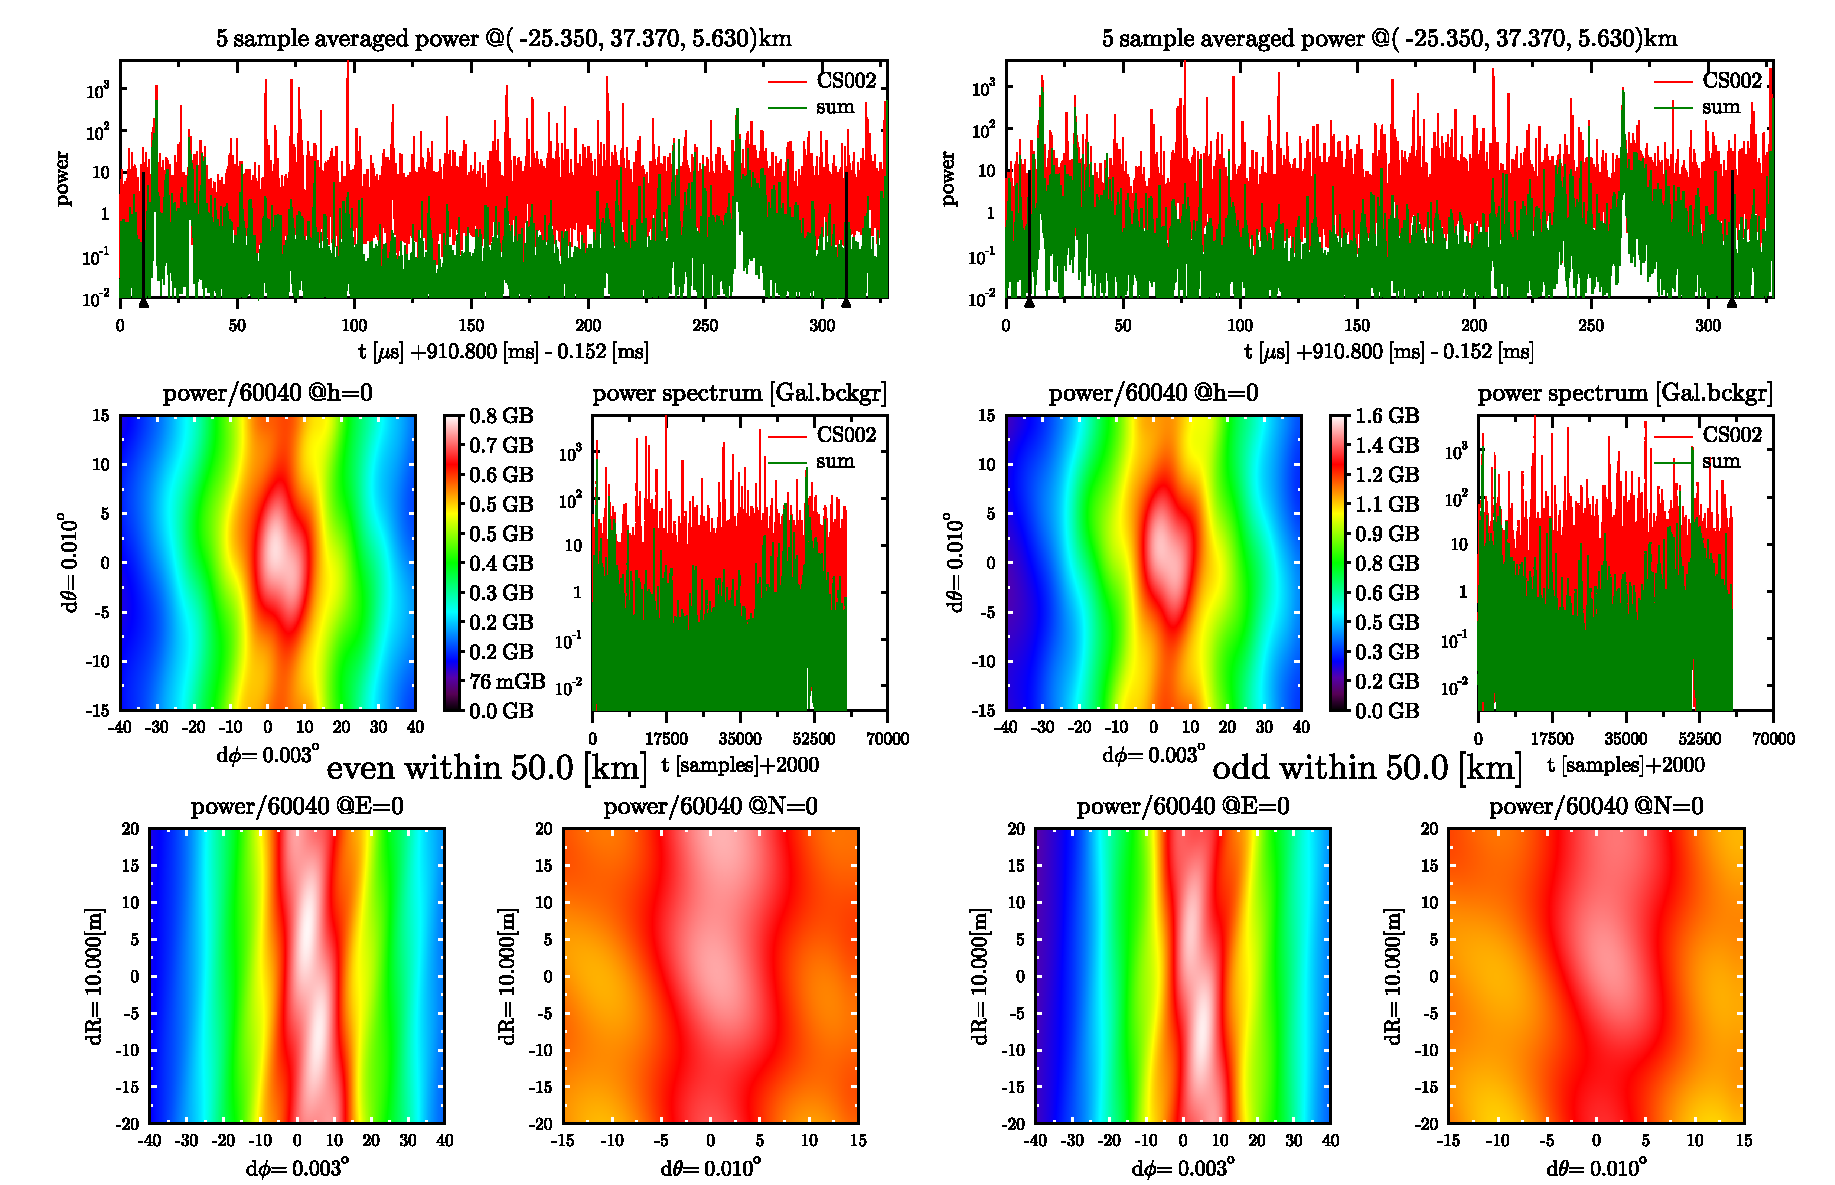
\includegraphics[width=0.99\textwidth]{Figs/InterfContourSE20A7-Np-} }
%\centering{\includegraphics[ bb=1.0cm 2.4cm 24.5cm 25.7cm,clip, width=0.49\textwidth]{../Figs/SE20A7-NPMx_1HIntfSpecSel} }
	\caption{Typical beamforming-intensity plot (name starting with `EIContour') as generated by running the TRI-D Imager.}	 \figlab{TRIDIntImg}
\end{figure}

A typical interferometric Intensity plot is shown in \figref{TRIDIntImg}. The data used for producing this plot are not saved.
\\Top panel: The time trace for the complete chunk of data in the reference antenna for the two dipoles. The selected time window for TRI-D imaging is indicated by the black triangles. For the case of \figref{TRIDIntImg} [line +3] reads `\verb!F   2000   1995 10.000 !' implying that the time window starts lies between sample 2000 or 10~$\mu$s and sample 3995 or about 20~$\mu$s. The time offset is written as the offset in the reference antenna plus the time difference with that at the center voxel.
\\middle left panel: The beamforming-intensity for the voxels at the central height. The axes in this plot give Easying and Northing with respect to the central voxel and the voxel size is shown on the axes. The intensity is integrated over the complete time window, listed on top of this panel.
\\middle central panel: The beamforming-intensity time trace for the central voxel summing the transverse (1+2) polarizations as seen from the core.
\\middle right panel: Showing (for the central voxel) the time trace for the transverse Stokes parameters, Q, U, V, normalized by the intensity. For a time trace with much background this plot is messy.
\\bottom left \& right panels: same as middle left panel for different cuts through the image cube.

\subsubsection{TRI-D Source position plot}\seclab{TRID-locate}

\begin{figure}[th]
\setlength{\unitlength}{.49\textwidth} % .43\textwidth}
   \subfloat[`IntfMx\_']{ \centering{\includegraphics[width=0.43\textwidth]{Figs/IntfMx_db-D3+05} } \figlab{TRIDSrcsImg}}
   \subfloat[`IntfPol\_']{ \centering{\includegraphics[bb=0.0cm 0cm 23cm 39cm,clip,width=0.43\textwidth]{Figs/IntfPol_db-D3+05} } \figlab{TRIDPolImg} }
%\centering{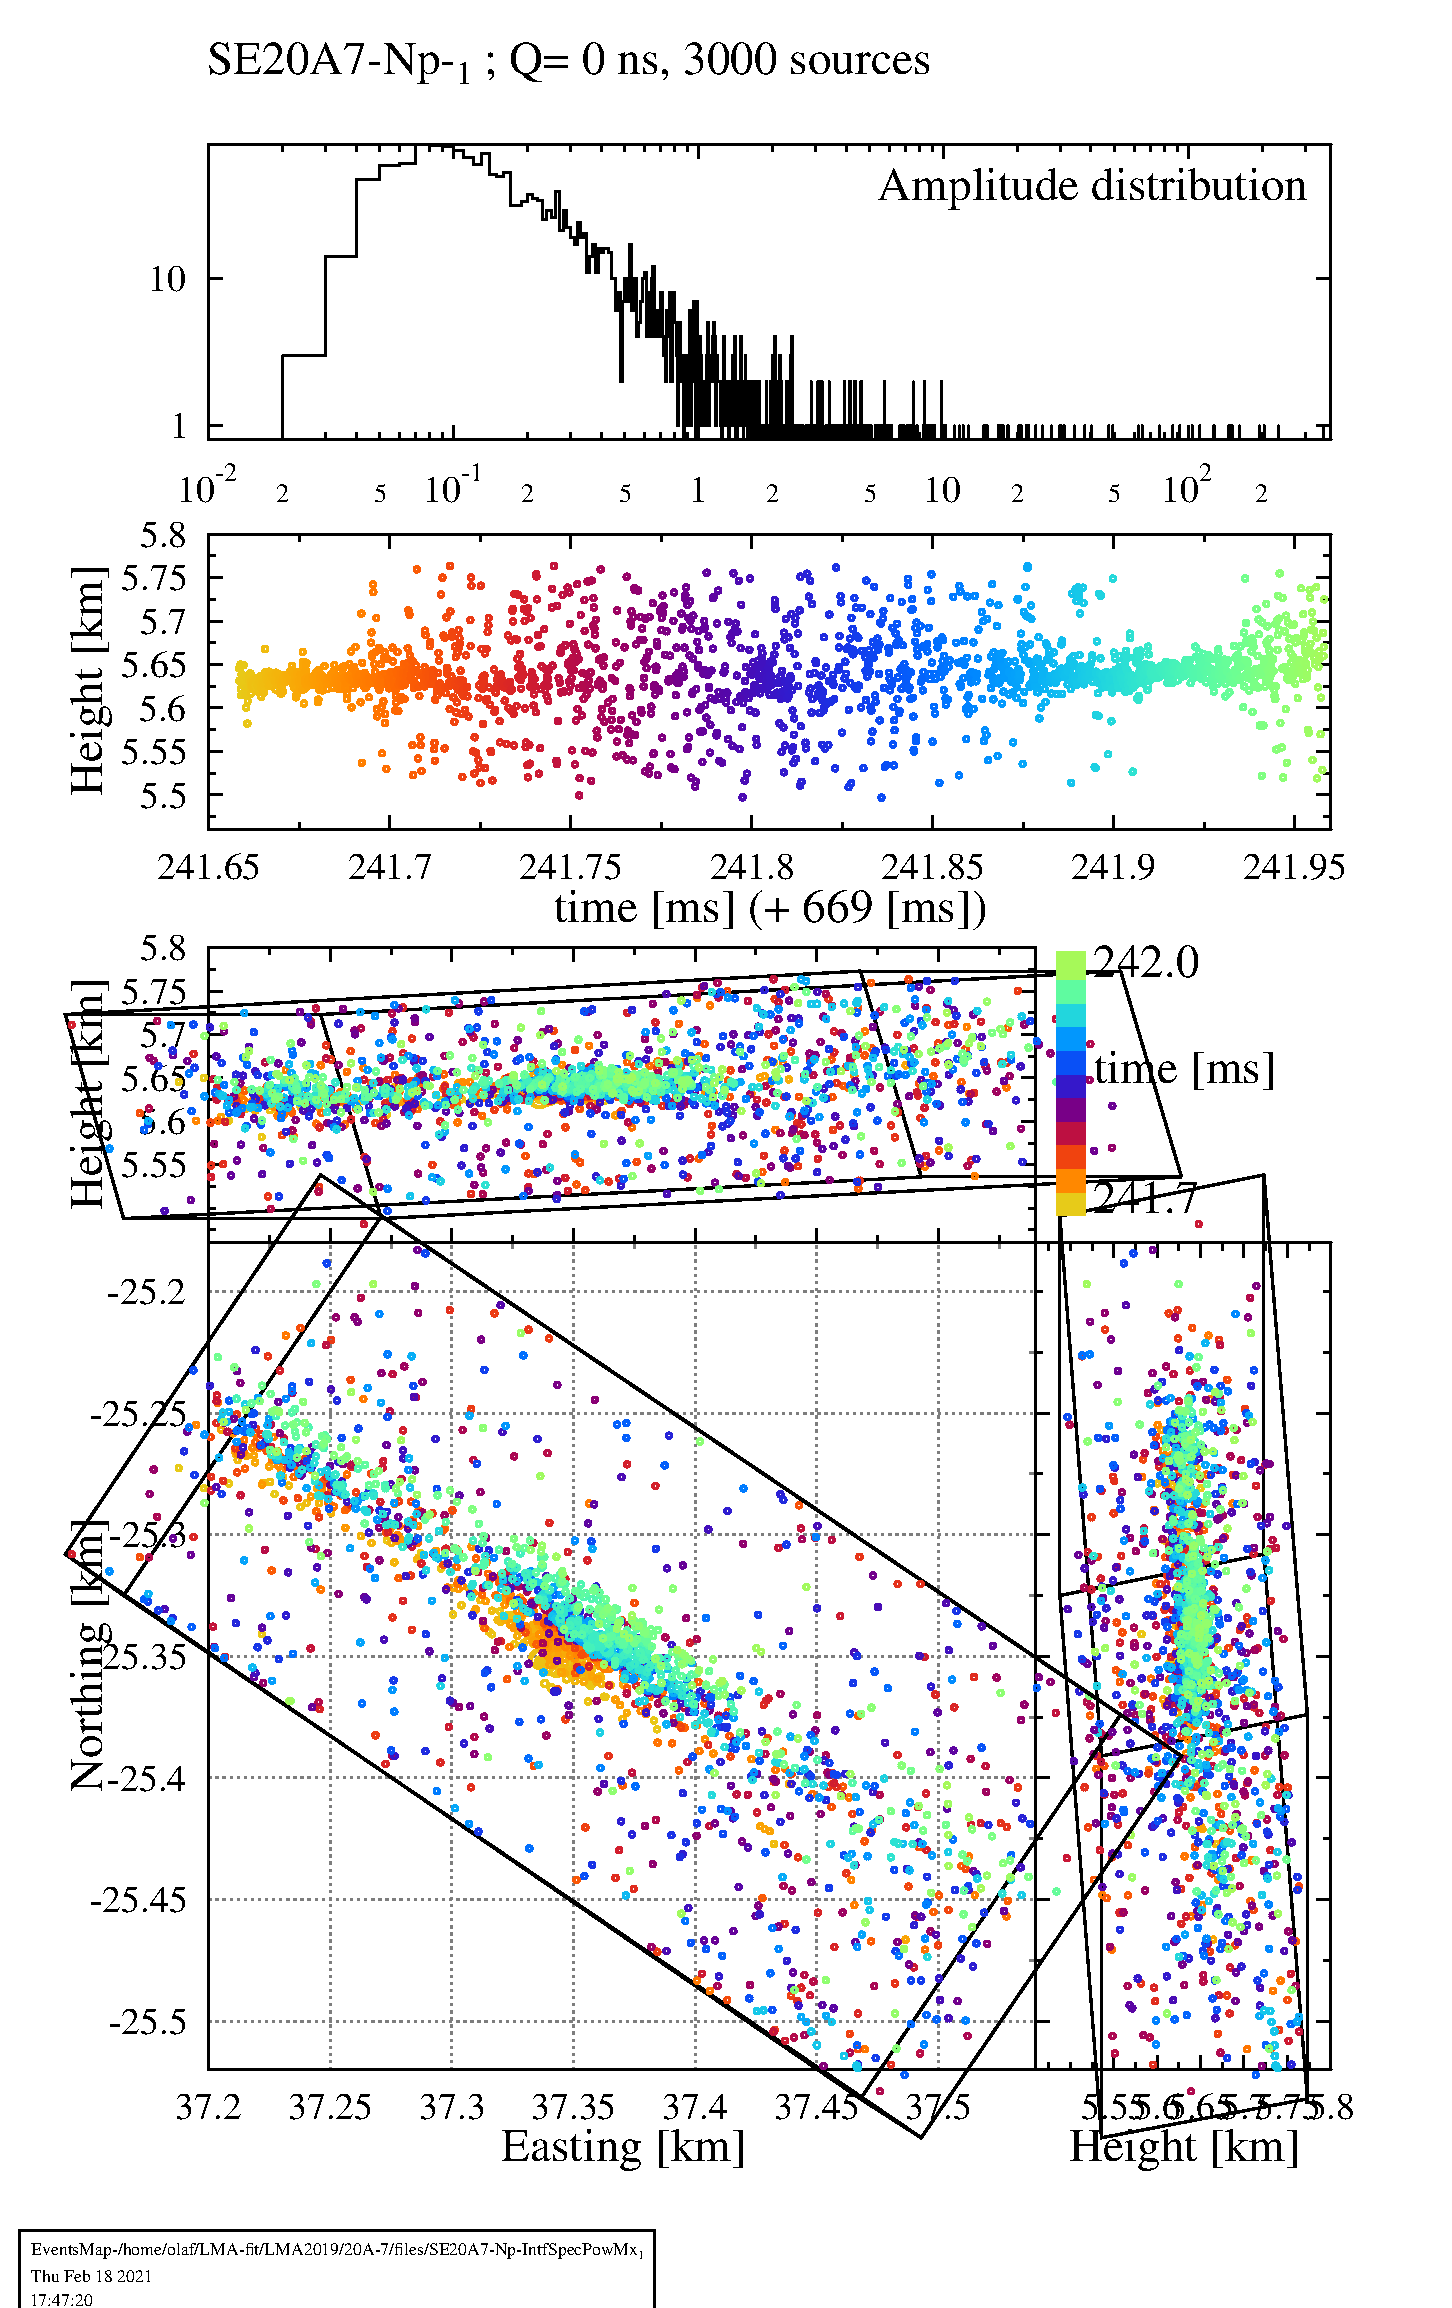
\includegraphics[width=0.49\textwidth]{Figs/SE20A7-Np--InfImaMx_1} }
%\centering{\includegraphics[ bb=1.0cm 2.4cm 24.5cm 25.7cm,clip, width=0.49\textwidth]{../Figs/SE20A7-NPMx_1HIntfSpecSel} }
	\caption{Plots generated by running the TRI-D imager where \figref{TRIDSrcsImg} shows a typical beamforming image plot (name starting with `IntfMx\_') and \figref{TRIDPolImg} a typical source polarization plot (name starting with `IntfPol\_').}	
\end{figure}

The located sources are given in \figref{TRIDSrcsImg} as well as the hypercube that was used for imaging. Sources close to the borders of this hypercube should not be trusted. The size of the wagon-wheels are a proxy for the relative intensities of the sources, where the size for the largest wagon-wheel is set by the 4$^{th}$ parameter on [line +3]. If negative, only dots are plotted and also the intensity plot (top panel) will be omitted.

The interferometric hypercube is also shown.

\subsubsection{TRI-D Source polarization plot}

A quick overview is presented of a variety of source-polarization observables. All are listed for each slice where the source obeyed the imaging conditions (not too close to the edge of the image cube, intensity above some threshold).
\\Top or 7$^{th}$ panel: the percentages of the linear, circular and unpolarized intensity.
\\6$^{th}$ panel: The $\chi^2$ of the fit to the time traces in all antennas for this slice. The $\chi^2$ tends to be large for strong peaks, implying that the error estimates on the trace amplitudes is not well under control and needs further scrutiny.
\\5$^{th}$ panel: The ratio of the intensity in the longitudinal (I3, as seen from the reference) direction compared to the total beamforming intensity as reconstructed by the imager. This ratio tends to be large for poorly reconstructed sources.
\\4$^{th}$ \& 3$^{rd}$ panels: The angular orientation of the dipole density per slice. For each slice a principal component analysis (PCA) is performed of the polarization directions per sample in the slice. Shown are the directions of the main (in red) and that of the secondary axes (in green) of the distribution. The error bars denote the amount of circular polarization. This is given as an error bar as one would expect that for a very long time trace the circular polarization should average to zero as there is -physics wise, because of symmetries- no reason for a net circular polarization. For short time traces the circular polarization will be non-zero due to random fluctuations. Note that the three axes are perpendicular.
\\2$^{nd}$ panel: Length of the three axes (red, green and yellow) if they are above a certain threshold.
\\bottom panel: The red line shows the summed transverse intensity for the reference antenna. The magenta dots give the transverse intensity for the slice at the source location. This should always be larger than that for the reference station in the default imaging conditions are used. The black dots show the total intensity, transverse + longitudinal, for the source.

\subsection{Selective plotting}\seclab{InterfSrcSel}

Note: This section in obsolete by now since the utility "InterfSrcSel" is superseded by "DataSelect" discussed in \secref{DataSelect}.

\Omit{ -------------------------------------------------------------
The script \verb!"InterfSrcSel.sh"! using \verb!"InterfSrcSel.in"! as input allows to produce plots that are zoomed in on the region of interest. This script plots the position of the sources using the GLE-script, \verb!"SourcesPlot.gle"! and the distribution of sources intensities using \verb!"SourcesPlot.gle"!. These are run via spawned scripts on Windows as well as Linux machines.
A typical input resembles:

\begin{linenumbers}
\resetlinenumber
\begin{verbatim}
&Parameters
 OutFileLabel="XYZ",     ! Normal Negative Leader (a)
 DataFile=   "SE20A7-Nh-", "SE20A7-Nh:-10", "SE20A7-Nh:-09", "SE20A7-Nh:-08", "SE20A7-Nh:-07", "SE20A7-Nh:-06"
   "SE20A7-Nh:-05"
 SMPowCut = 3.,       ! power of pulse included in the plot
 AmpltPlot=0.1       !  dependence of dot sizes on pulse power
 MaxAmplFitPercent=0.001      ! Maximal percentile amplitudes to be included in fits of power-spectrum
 ZoomClip = .true.   ! clip sources outside plotting region
 xmin=37.15 , xmax=37.6, ymin=-25.45, ymax=-25.15, zmin=5.35, zmax=5.8,  tmin=237.0 , tmax=245.3
&End
\end{verbatim}
\end{linenumbers}

The lines in the namelist \verb!"&Parameters"! input specify:
\begin{enumerate}
\item[2] \verb!"OutFileLabel="!: Additional label used for the output files, including the plots.
\item[3] \verb!"DataFile="!: Distinctive \verb!"XYZ"! labels of the data files discussed in \secref{InterfSrc}. The data of all these files will be sorted in time and used for plotting and producing the intensity distributions.
\item[5] \verb!"SMPowCut="!: Only stronger sources are used for plotting.
\item[6] \verb!"AmpltPlot="!: A factor used for scaling the dot-size when plotting. If zero all dots are the same size.
\item[7] \verb!"MaxAmplFitPercent="!: Percentile cut for the sources included in fitting a power-law to the distribution. Stronger sources are excluded.
\item[8] \verb!"ZoomClip="!: Clip source locations to the plotting volume.
\item[9] \verb!"xmin="!: The bounding boxes used in space and time for the plots.
\end{enumerate}

\begin{figure}[th]
\centering{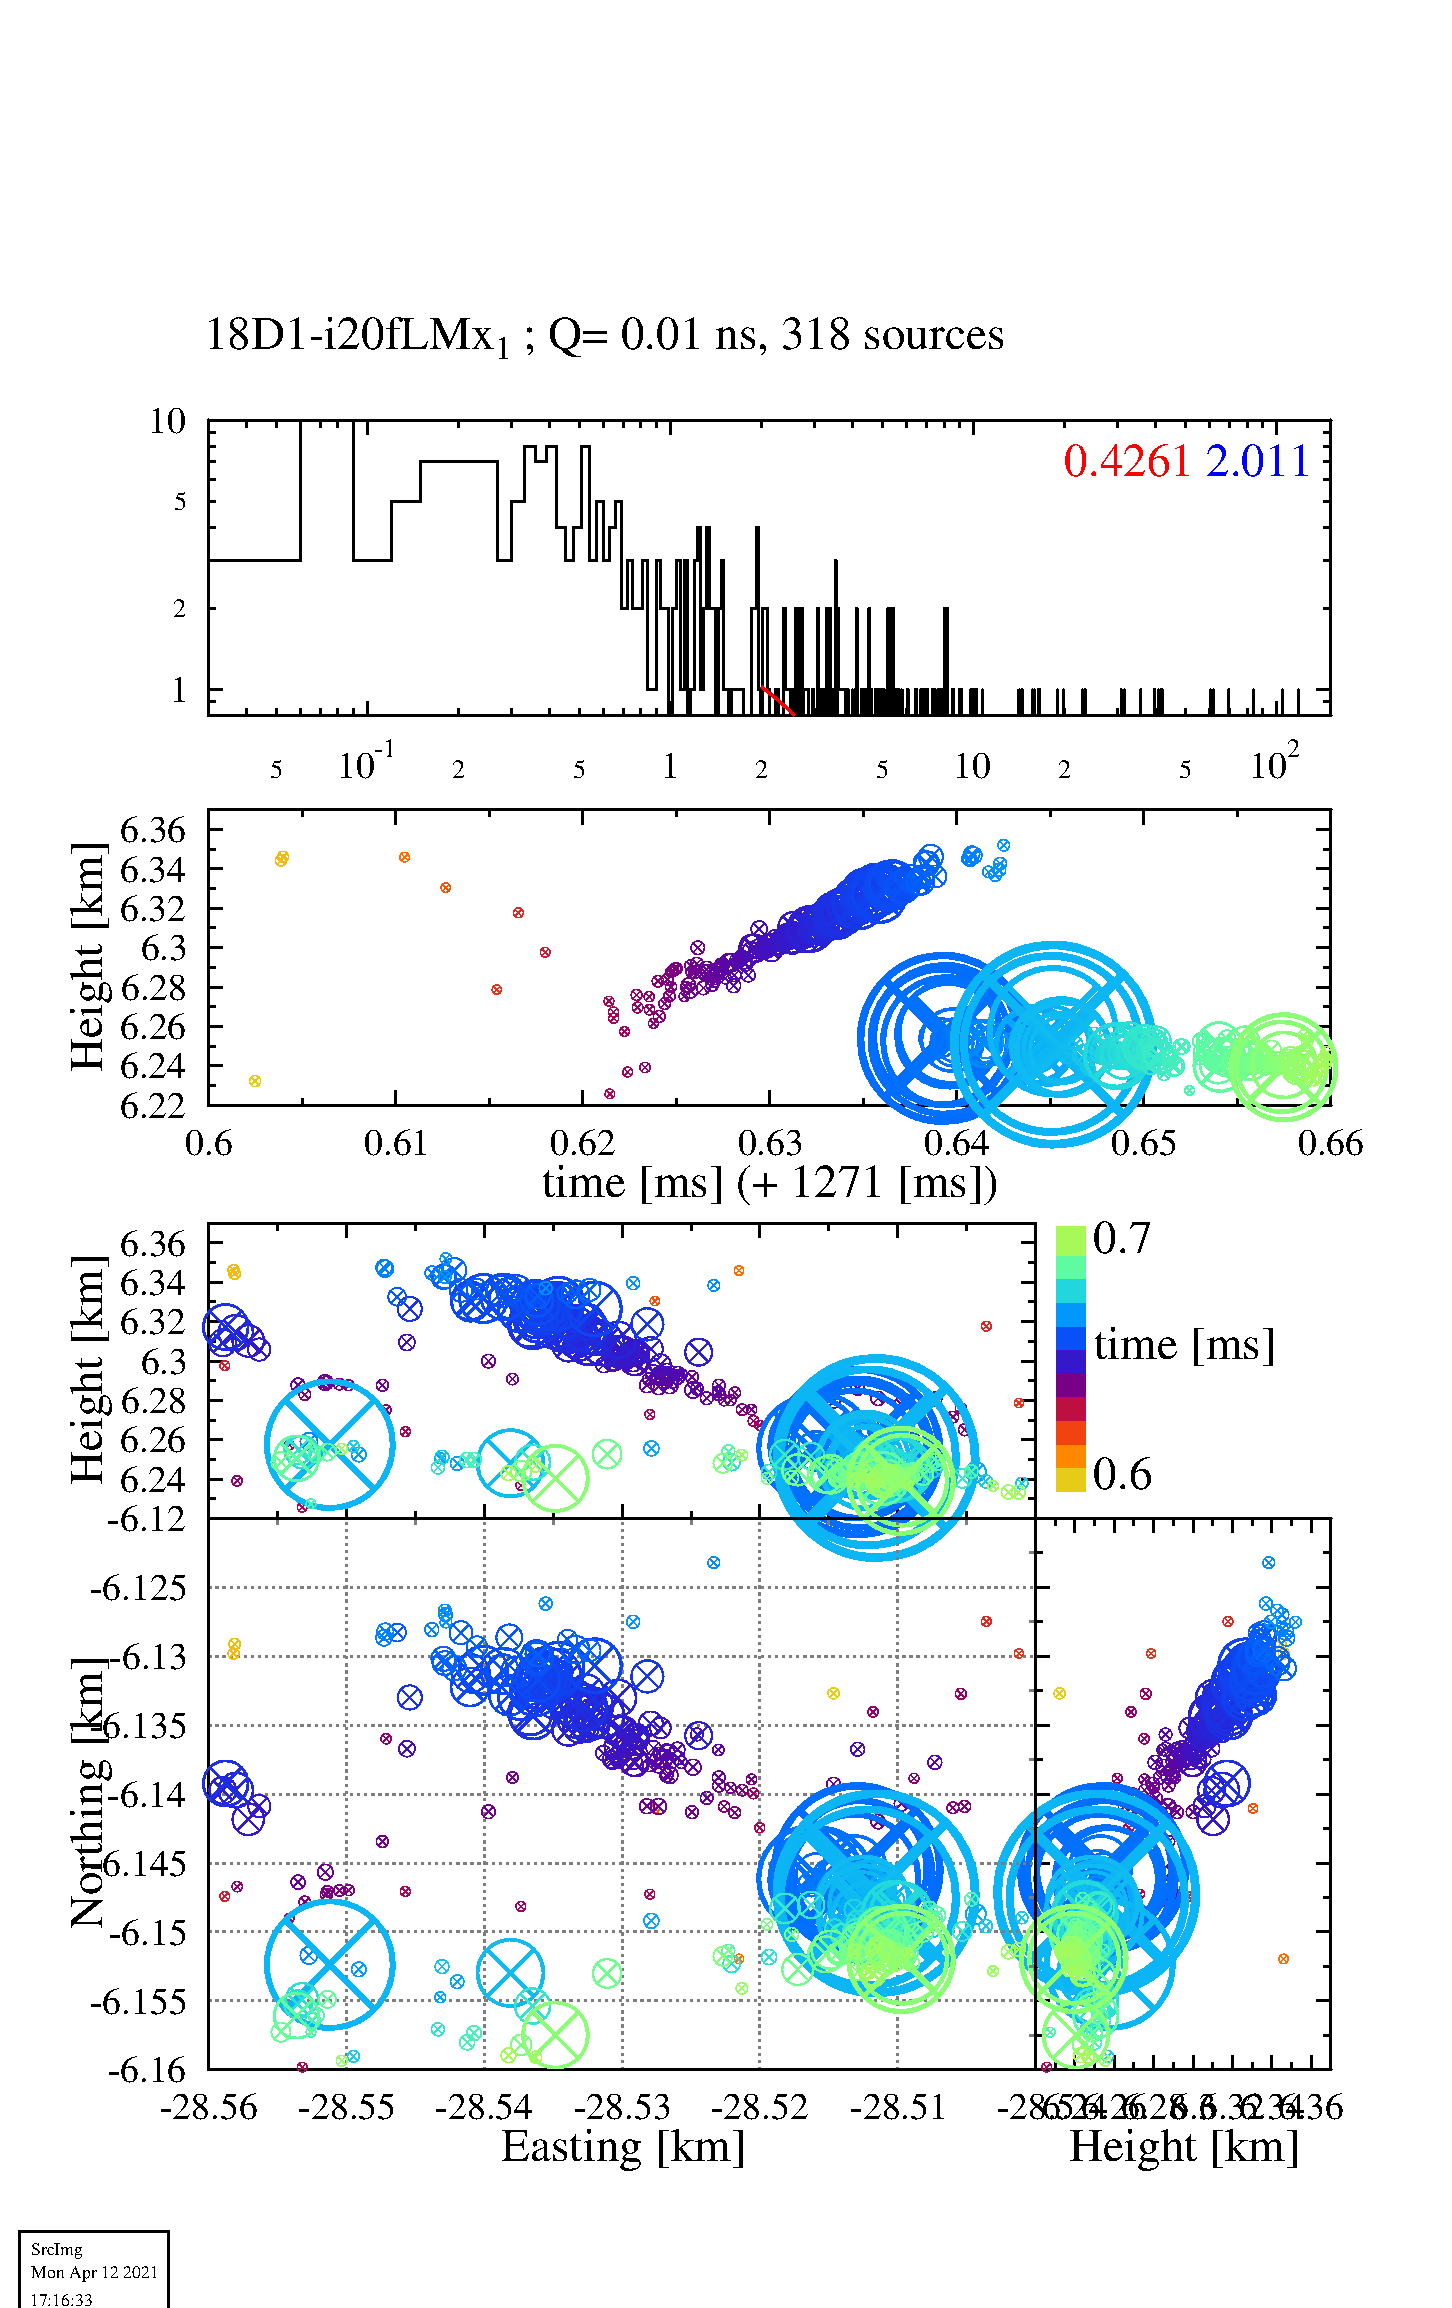
\includegraphics[width=0.49\textwidth]{Figs/18D1-i20fMx_1LIntfSpecSel} }
%\centering{\includegraphics[ bb=1.0cm 2.4cm 24.5cm 25.7cm,clip, width=0.49\textwidth]{../Figs/SE20A7-NPMx_1HIntfSpecSel} }
	\caption{Typical image for the TRID Imager as created by running ``InterfSrcSel.sh".}	 \figlab{TRIDSelSrcsImg}
\end{figure}

The plots will be made for the `Mx' and `Bar' files as well as for X- and Y-dipoles, all resembling \figref{TRIDSelSrcsImg}. This allows for appending seamless the results of different interferometry runs.

} %---------------------------------------------------------------------

\clearpage
\section{The `SelectData' option}\seclab{SelDat}

To create the appropriate files containing antenna positions used for the simulated data as well as to select the portion of the traces that require focussed attention it is necessary to run the script \verb!SimDataSU.sh!. The script reads the input data from \verb!SimData.in!.
The antenna data are in particular necessary for running data simulations, \secref{Sim}, to explore the sensitivity of the antenna layout.
Typical input lines are

\begin{linenumbers}
\resetlinenumber
\begin{verbatim}
&Parameters
 RunOption= "SelectData"
 Simulation="simulation/S1-1"  ,
! TimeBase=1221
 AntennaRange=100  ! [km]
 Calibrations="Calibrations202202011947.dat" ! 
 BadAnt_SAI=     1072,   1073,   3054,   3055,   6072,   6073,  21072,  32072, 101090, 121048
               121049, 121054, 121055, 121062, 121063, 121072, 121073, 121084, 121085, 121091
               142048, 142049, 125062, 125063, 130072, 130073, 145048, 161084, 181055, 188054
               188055,  32049   
 SignFlp_SAI=   161072, 161073,
!  OutFileLabel="CalSrc"
 &end
     1550.   20.44193   8.86218   1.55186 !
M    10547 250   !
\end{verbatim}
\end{linenumbers}


\begin{enumerate*}
\item[2] \verb#` RunOption= "SelectData"'#: The run-option.
\item[3] \verb#` Simulation="simulation/S1-1" '#:  The place in the "files" folder where the simulation results are written. If necessary the subfolder (recommended) is created.
\item[4-13] These parameters have the usual meaning.
\item[14] \verb#` 1550.   20.44193   8.86218   1.55186 '#:  time (at the source position) and position (N,E,h). 
\item[15] \verb#`M    10547 250 '#: First sample number in the selected data chunk (=10547) and number of samples (=250) copied to a separate file. In case of mark `M' not the first, but the median sample (=10547) is given. 
\end{enumerate*}


\subsection{output and print-out}\seclab{SelDat-out}

The print out \verb!SelectData.out! is very self-explanatory.

Several files are created in the sub-folder \verb!files! following the naming convention as specified by the `Simulation' parameter. The files that contain LOFAR antenna-stations in their names specify the antenna positions for this station as well as the selected part of the trace, cleaned from RFI. The \verb!..._Structure.dat! just list the stations that are active. These files are expected to be present for running simulation calculations as discussed in \secref{Sim} and may be edited at your own risk.

The time traces are corrected for antenna calibrations and the antenna-time offsets (as given in the antenna files) are to correct for source location.

The generated files will be used as input when running the impulsive of the TRI-D imager with option \verb!`Simulation="simulation/S1-1" '!.
\chapter{Supplementary scripts}\seclab{supp}
\section{Plotting flashes}\seclab{DataSelect}

The raw lists of sources as generated by the impulsive and the TRI-D imagers of the LOFLI package are post-processed to produce images of the flash and supplementary data. The main objective is to select from the raw source files those sources that obey certain quality conditions (like the value of the chi-square for the impulsive imager) and fall within the designated time span and box in the atmosphere. It allows for tracking a leader and produce the distribution of the sources around the leader among other aspects.

The LINUX script \verb!DataSelect.sh! reads the input from DataSelect. The script \verb!DataSelect.bat! is for running under windows and uses the same input. Note that this script combines the functionality of the older scripts \verb!FlashImage! and \verb!InterfSrcSel!.

In its most basic form \verb!DataSelect.in! reads like

\begin{linenumbers}
\resetlinenumber
%\small
\footnotesize
%\scriptsize
%\tiny
\begin{verbatim}
&Parameters
datafile= "Srcs23-evenn", xyztBB= 15.75 +17.8  40 42.  3.5 5.5   1965 1990 ,  PlotName= "3b-N1"
&End
\end{verbatim}
\end{linenumbers}

A parameter block starts with \verb!&Parameters! and ends with \verb!&end! where the different parameters are separated by commas, and may spread over several lines. An input file can contain several parameter blocks. The most basic parameters are:
\begin{enumerate*}
\item \verb!datafile= "filename"!: specifying the name of the file that contains the list of raw sources. The quotation marks are essential and the extension is added automatically. The file should reside in the same folder where \verb!DataSelect! is run or otherwise the filename should contain the path. If the file in the folder has the extension \verb!.csv! is implies that the raw sources are generated by the impulsive imager.
\item \verb!xyztBB=!: followed by eight real values specifies the bounding box for the image. The expected order is minimum and maximum values for the x coordinate, followed by those for y, z, and time.
\item \verb!PlotName= "xxx"!: The names of all plots will be composed of three parts, first the name of the folder (impulsive imager, usually equal to the flash name) or the name of the datafile (TRI-D imager), followed by \verb!xxx!, and possibly followed by the name of a special purpose plot.
\end{enumerate*}
The complete list of possible parameters with a short explanation can be found in the \verb!DataSelect.out! file. Note that some options are specific for either impulsive imager data or for TRI-D data. We will discuss the different parameters as they are used for for various options.

\subsection{Flash image}

For generating a flash image the following parameters may also be important, beside the basic ones.

Specific options when using data from the impulsive imager, with their default value. All determine the quality conditions a source should obey to be plotted.
\begin{enumerate*}
\item \verb!RMS_ns= 4.0!: condition [$\sqrt(\chi^2) <$ \verb!RMS_ns!] in units [ns].
\item \verb!DelNEff= 25 ! (integer): condition when [\verb!DelNEff! $>0$] is [(\# of available antennas) - (\# number of used antennas)) $\leq$ \verb!DelNEff! ], where (\# of available antennas) is the number of antennas that have data for this source and (\# number of used antennas) is the number of antennas where the pulse from this source could be identified unambiguously.
\item \verb!LinCutH= 2.0!: condition: [$\sigma_h \times h <$ \verb!CutSigmaH! $\times$ \verb!LinCutH!] when [$h < $\verb!LinCutH!], unit [km], where $\sigma_h$ is the error in the altitude of a source as estimated by the impulsive imager at altitude $h$. The error in altitude is usually larger than those in Northing or Easting of the source. Additionally it is seen that this error grows with the altitude of the source which is the reason for the linear dependence. This quality indicator is particularly important when imaging ground strokes.
\item \verb!CutSigmaH= 17.0!: see above.
\item \verb!QualPlot= F !(logical): make a scatter plot of different quality indicators to investigate their correlations.
\end{enumerate*}

Specific options when using data from the TRI-D imager, with their default value:
\begin{enumerate*}
\item \verb!datafile= "xxx#+", "yyy" !: The \verb!"OutFileLabel="! from the different TRI-D runs for which the images have to be merged. This may also be just from a single run. The \verb!"#+"! in the name indicates that all files are collected that were generated by the TRI-D imager when it followed a leader path.
\item \verb!TimeBase=!: the default value is taken from the first file that is read.
\item \verb!SMPowCut= 500.0!: plot only those sources for which the intensity exceeds the specified limit.
\item \verb!StatNCut= F! (logical): keep only the ``\verb!FileStatN!" strongest sources of each TRI-D source file. This functions as a simple way to set a variable intensity threshold when a dart leader drastically changes its intensity as it propagates.
\item \verb!FileStatN= 5 !:Print the strength of the N$^{th}$ strongest source in the .out file. This was most useful for the estimate of the upper strength of positive leaders in Ref.~\cite{Scholten:2023PL}.
%\item[4] \verb!"! ZoomClip = .true."!: Only the points falling inside the plot boundary will be drawn.
\end{enumerate*}
When in \verb!datafile=! multiple source files are specified, these data will be merged and written to file. This file will have \verb!repack! in its name.


Some Generic options when using data from both imagers, with their default value:
\begin{enumerate*}
\item \verb!tCutl= 0.0!: lower end of block filter in time.
\item \verb!tCutu= 0.0!: upper end of block filter in time. This allows for blocking-out a single bright source that may even be outside the windowed area, but enters the picture through `side beams'.
\item \verb!BckgrFile= ""!: name of file that is displayed as a grey background plot.
\item \verb!ZoomBox= "NoBox" !:  name of the plot that zooms-in on a section of the present plot. This produces a box in the figure indicating the zoomed-in area. This option is used frequntly, see for example Ref.~\cite{Scholten:2021-HANL}.
\item \verb!AmplitudePlot=!  (Imp: =-1.00 ; TRI-D: =10.0): it sets the diameter of the largest symbols used in the plot. When zero or negative, a fixed size dot will be used for all points, independent of their intensity. Additionally the panel showing the intensity spectrum will not be shown.
\item \verb!NEhtBB=!: an alternative way to specify the bounding box using Northing, Easting, Altitude, and Time.
\end{enumerate*}


\begin{figure}[th]
\centering{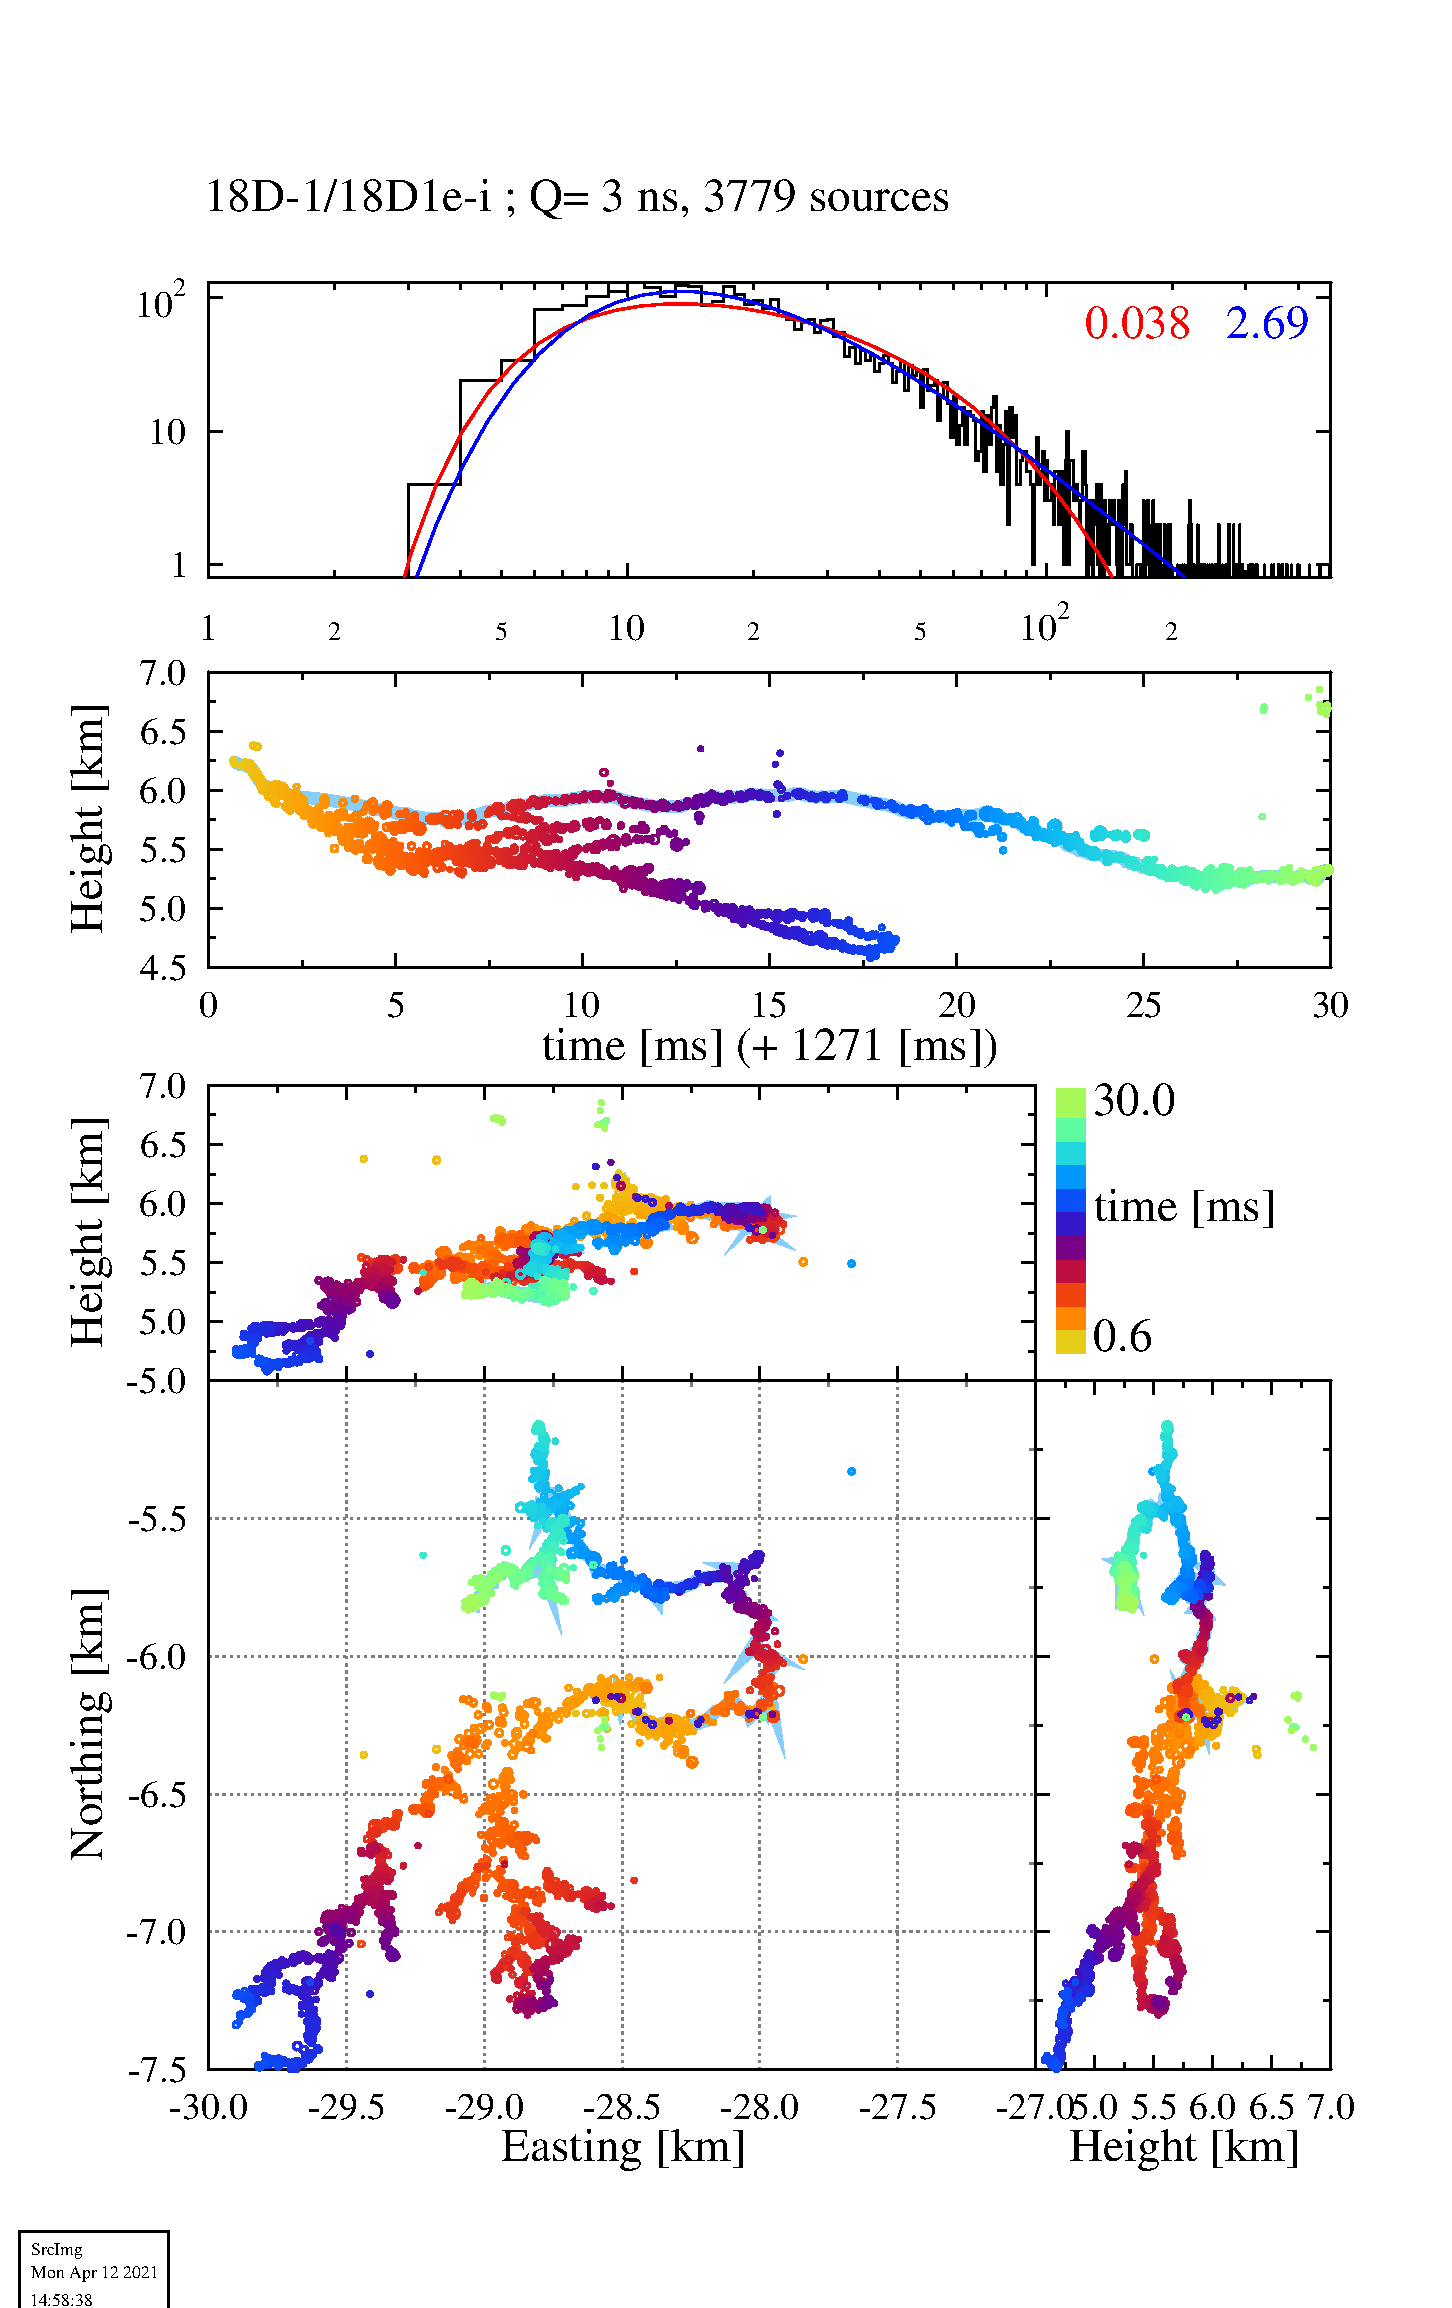
\includegraphics[width=0.49\textwidth]{Figs/Imp_18D1e-i} }
\centering{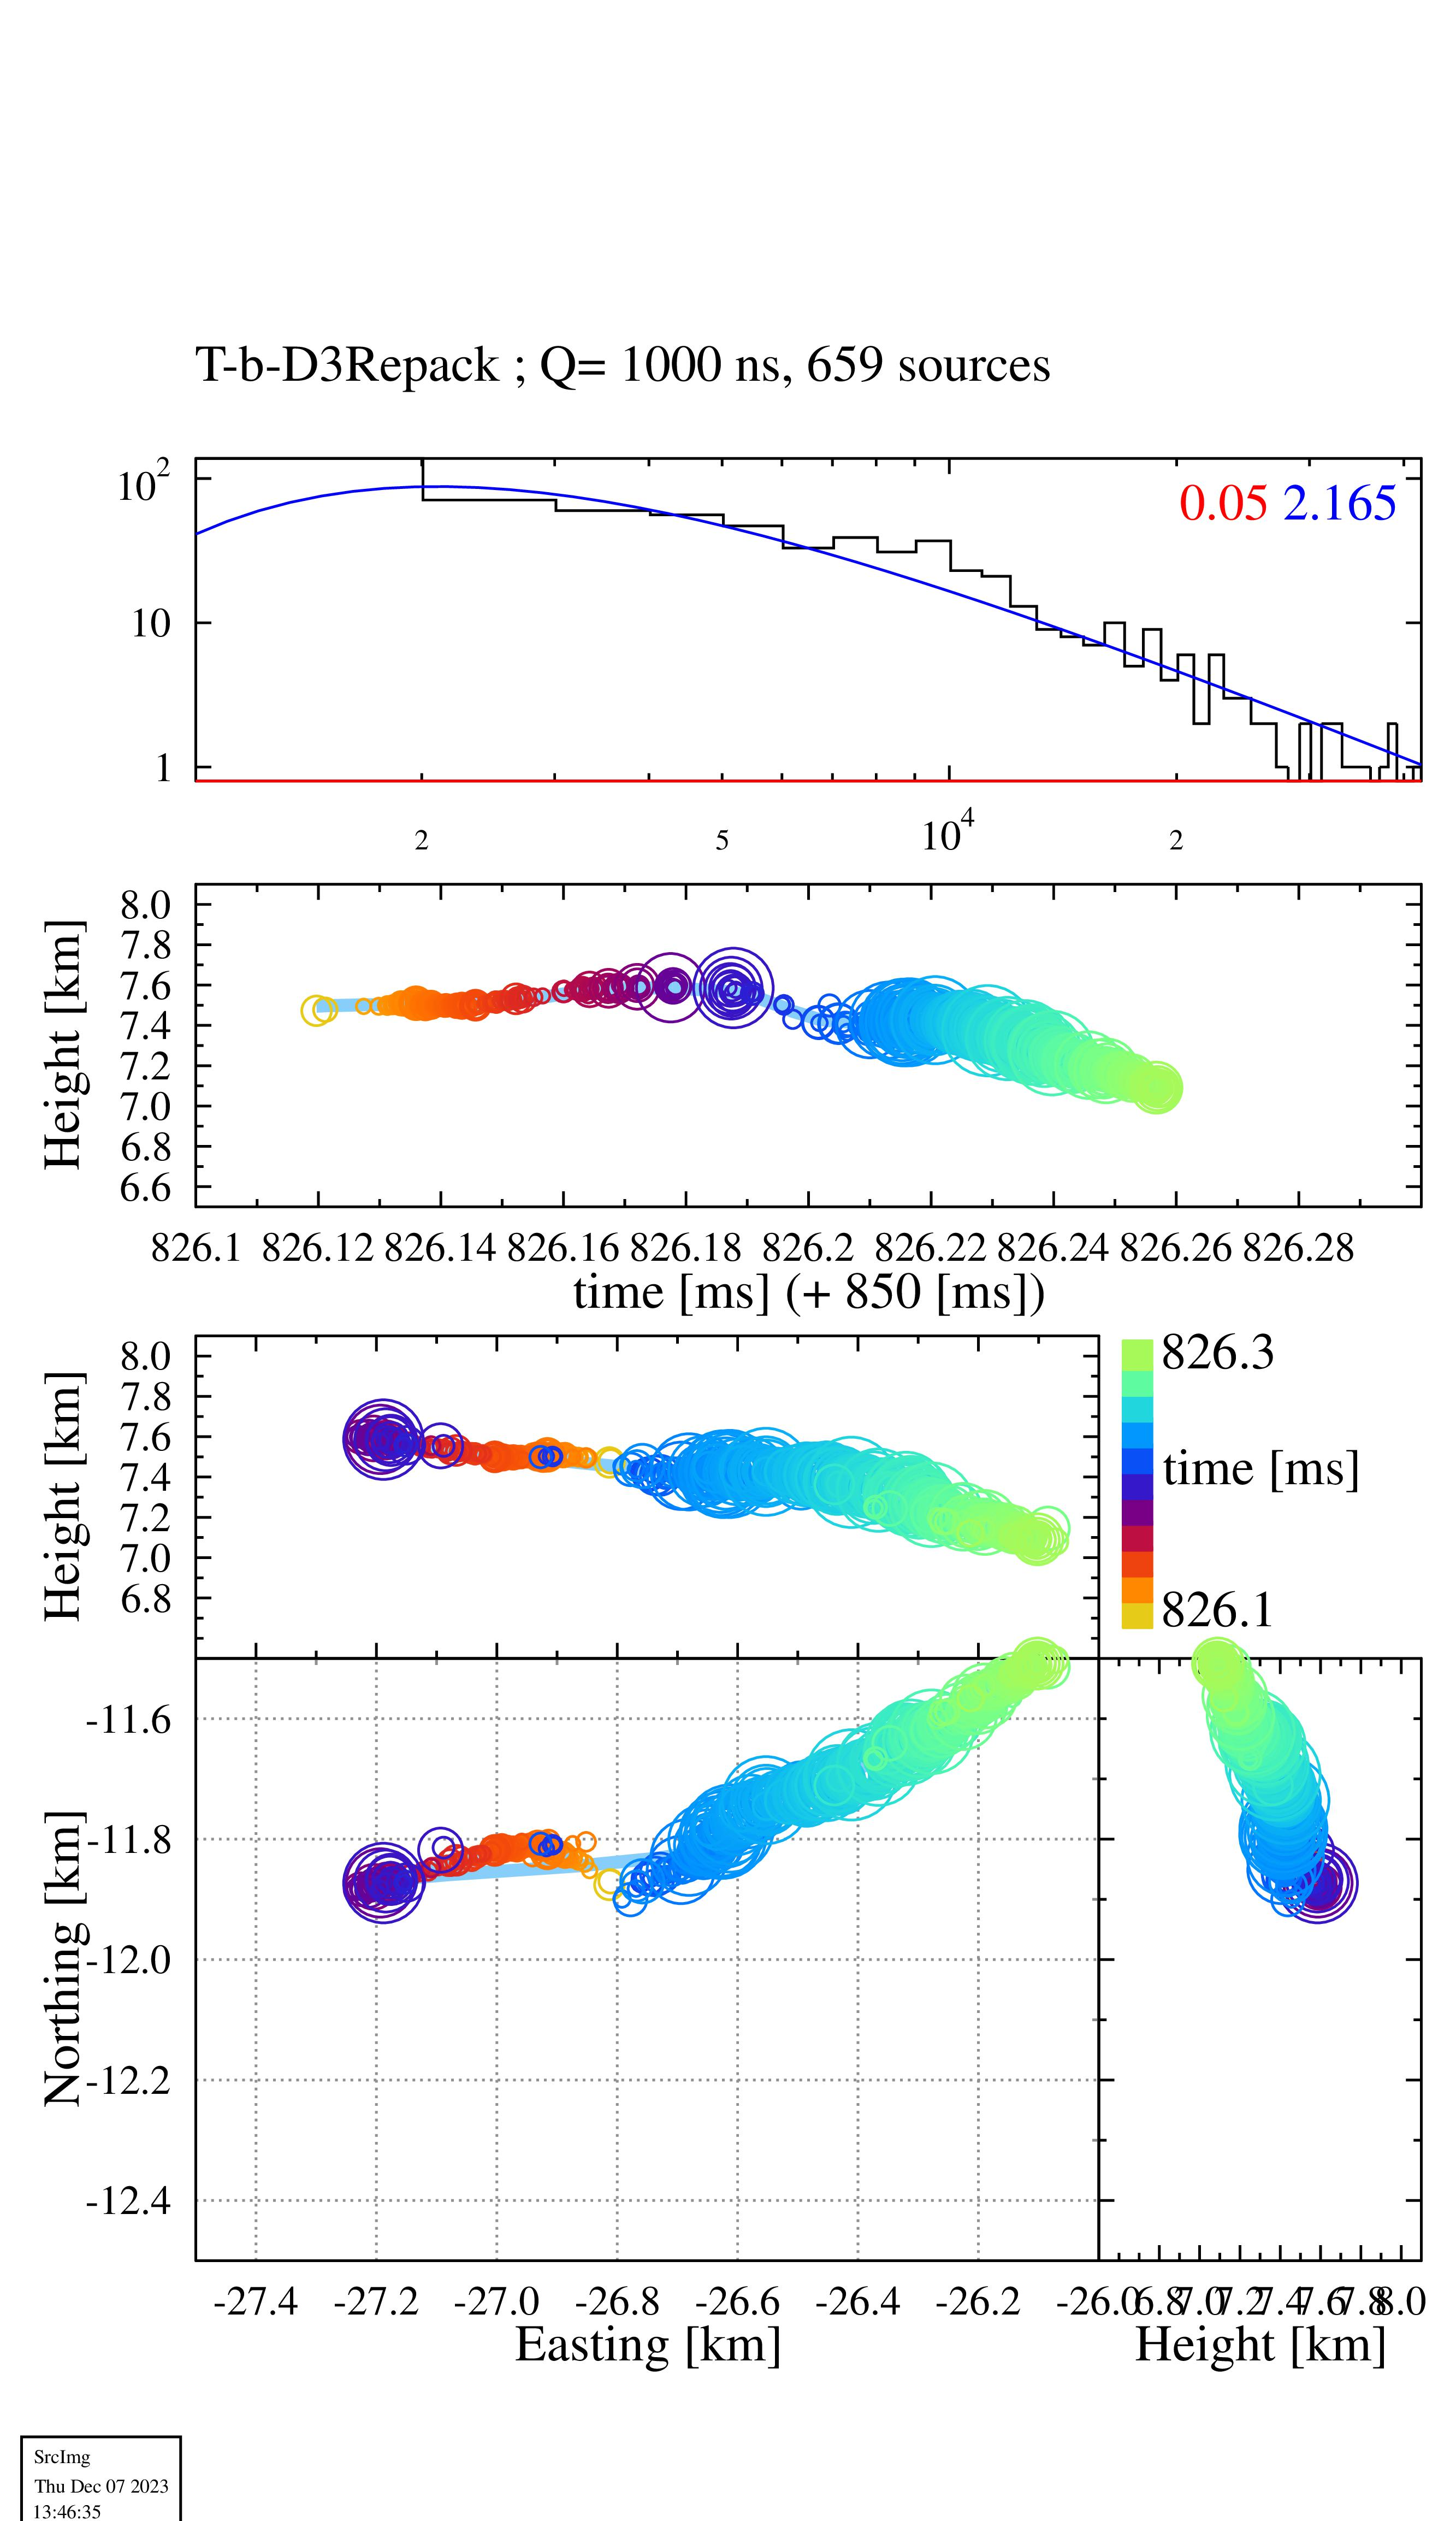
\includegraphics[width=0.49\textwidth]{Figs/T-b-D3Repack} }
%\centering{\includegraphics[ bb=1.0cm 2.4cm 24.5cm 25.7cm,clip, width=0.49\textwidth]{../Figs/SE20A7-NPMx_1HIntfSpecSel} }
	\caption{Typical image for the Impulsive Imager (left) and the TRI-D imager (right) as created by running ``DataSelect.bat". Light blue band is the reconstructed track (starting from the latest point and tracing back). Top panel give pulse power statistics where the modified exponential is plotted in red and the modified power law plotted in blue.}	 \figlab{ImpulsiveImg}
\end{figure}


The produced .dat files are plain text files and contain some header lines with some general information followed by the specific data of the sources. The files have a format that is suitable for the plotting script \verb!"SourcesPlot.gle"!.


Two gle-scripts \verb#'%UtilDir%Intensity.gle'# and \verb#'%UtilDir%SourcesPlot.gle'# make the following plots.

\begin{figure}[h]
\setlength{\unitlength}{.48\textwidth} % .43\textwidth}
   \subfloat[Figure `IntfSpecSel']{ 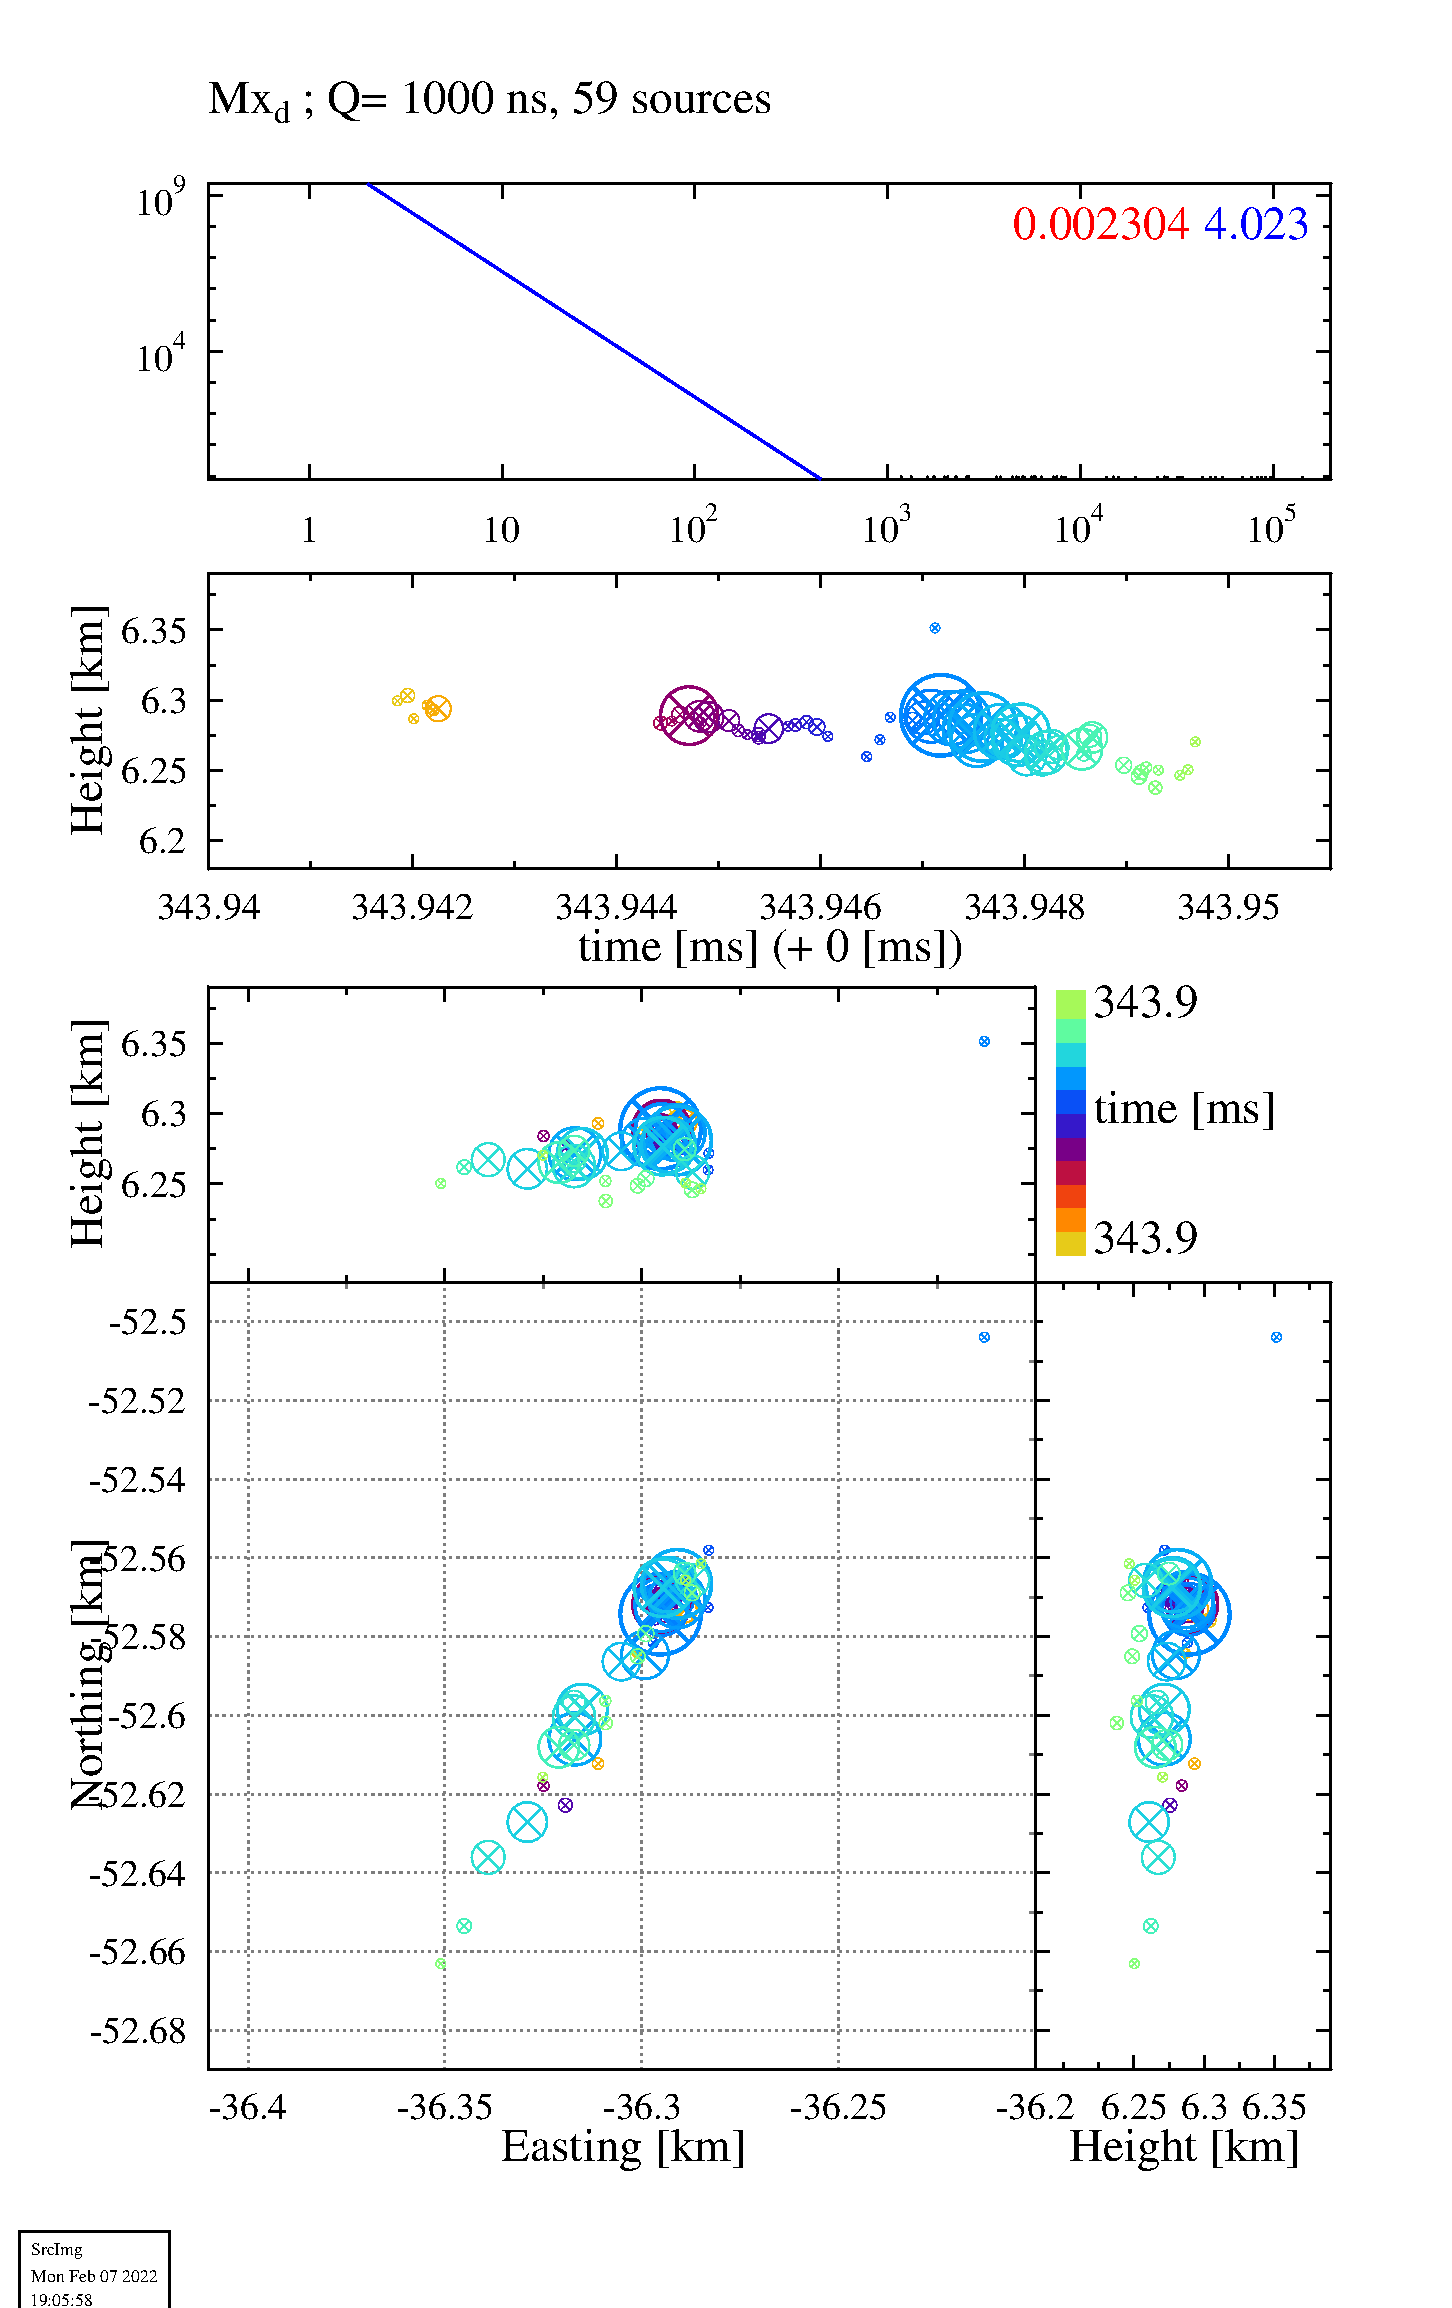
\includegraphics[width=\unitlength]{Figs/Mx_dIntfSpecSel}  \figlab{InterfSrc-Spec}}
   \subfloat[Figure `AmplFit']{ 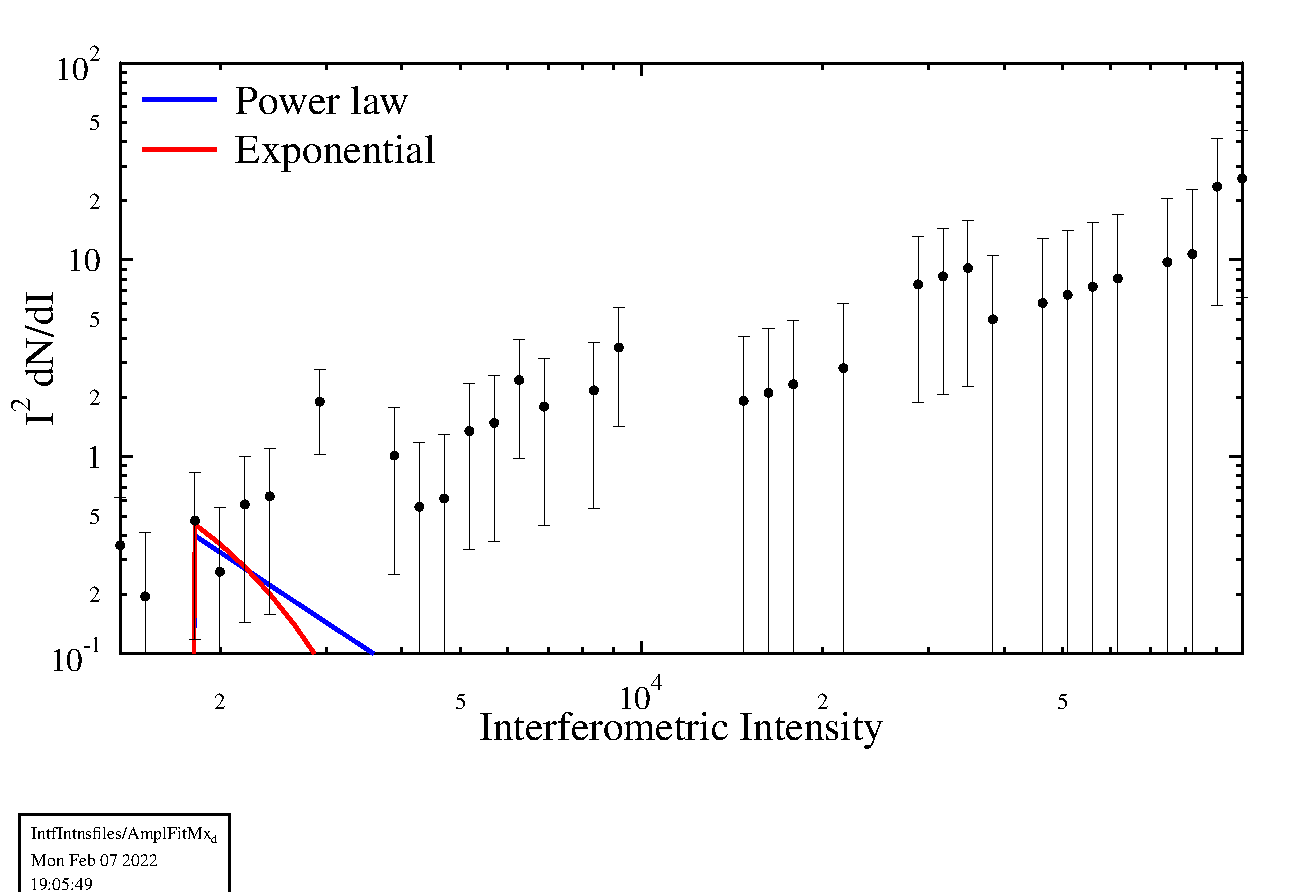
\includegraphics[width=\unitlength]{Figs/Mx_dAmplFit}  \figlab{InterfSrc-Ampl}}
	\caption{Top panel in \figref{InterfSrc-Spec} shows the intensity distribution of the sources and two fits (that obviously do not resemble the data for this case). The lower panels the usual way of plotting the sources where the size of the circles reflects the intensity.
\figref{InterfSrc-Ampl} displays an attempt to fit the pulse-strength distribution.}	 \figlab{InterfSrc}
\end{figure}

Obviously more writing needs be done, but this is it for the time being.

\subsection{Track finding}

Produces, among other aspects of a leader, the velocity distribution along the leader track as used in Ref.~\cite{Scholten:2021-RNL}

Some Generic options when using data from both imagers, with their default value:
\begin{enumerate*}
\item \verb!NLongTracksMax= 0 !: Maximum number of tracks to include in plot
\item \verb!MaxTrackDist= !: Max. distance between sources to include on a track.
\item \verb!Wtr=!: Weight of newest source for track centroid.
\item \verb!Aweight= 0.0!: Importance of intensity in weight of newest source for track centroid.
\item \verb!TimeWin=!: [ms]. Width of gaussian in time to weigh the sources for mean track position.
\item \verb!PreDefTrackFile= ""!: Label of file that contains a track to be included.
\item \verb!dt_MTL=!: [ms]. Time-step for constructing tracks.
\item \verb!HeightFact= 0.0!: Relative height scale for calculating distances.
\item \verb!SrcDensTimeResol=!: [ms]. Source Density Time Resolution.
\end{enumerate*}


\begin{figure}[th]
\centering{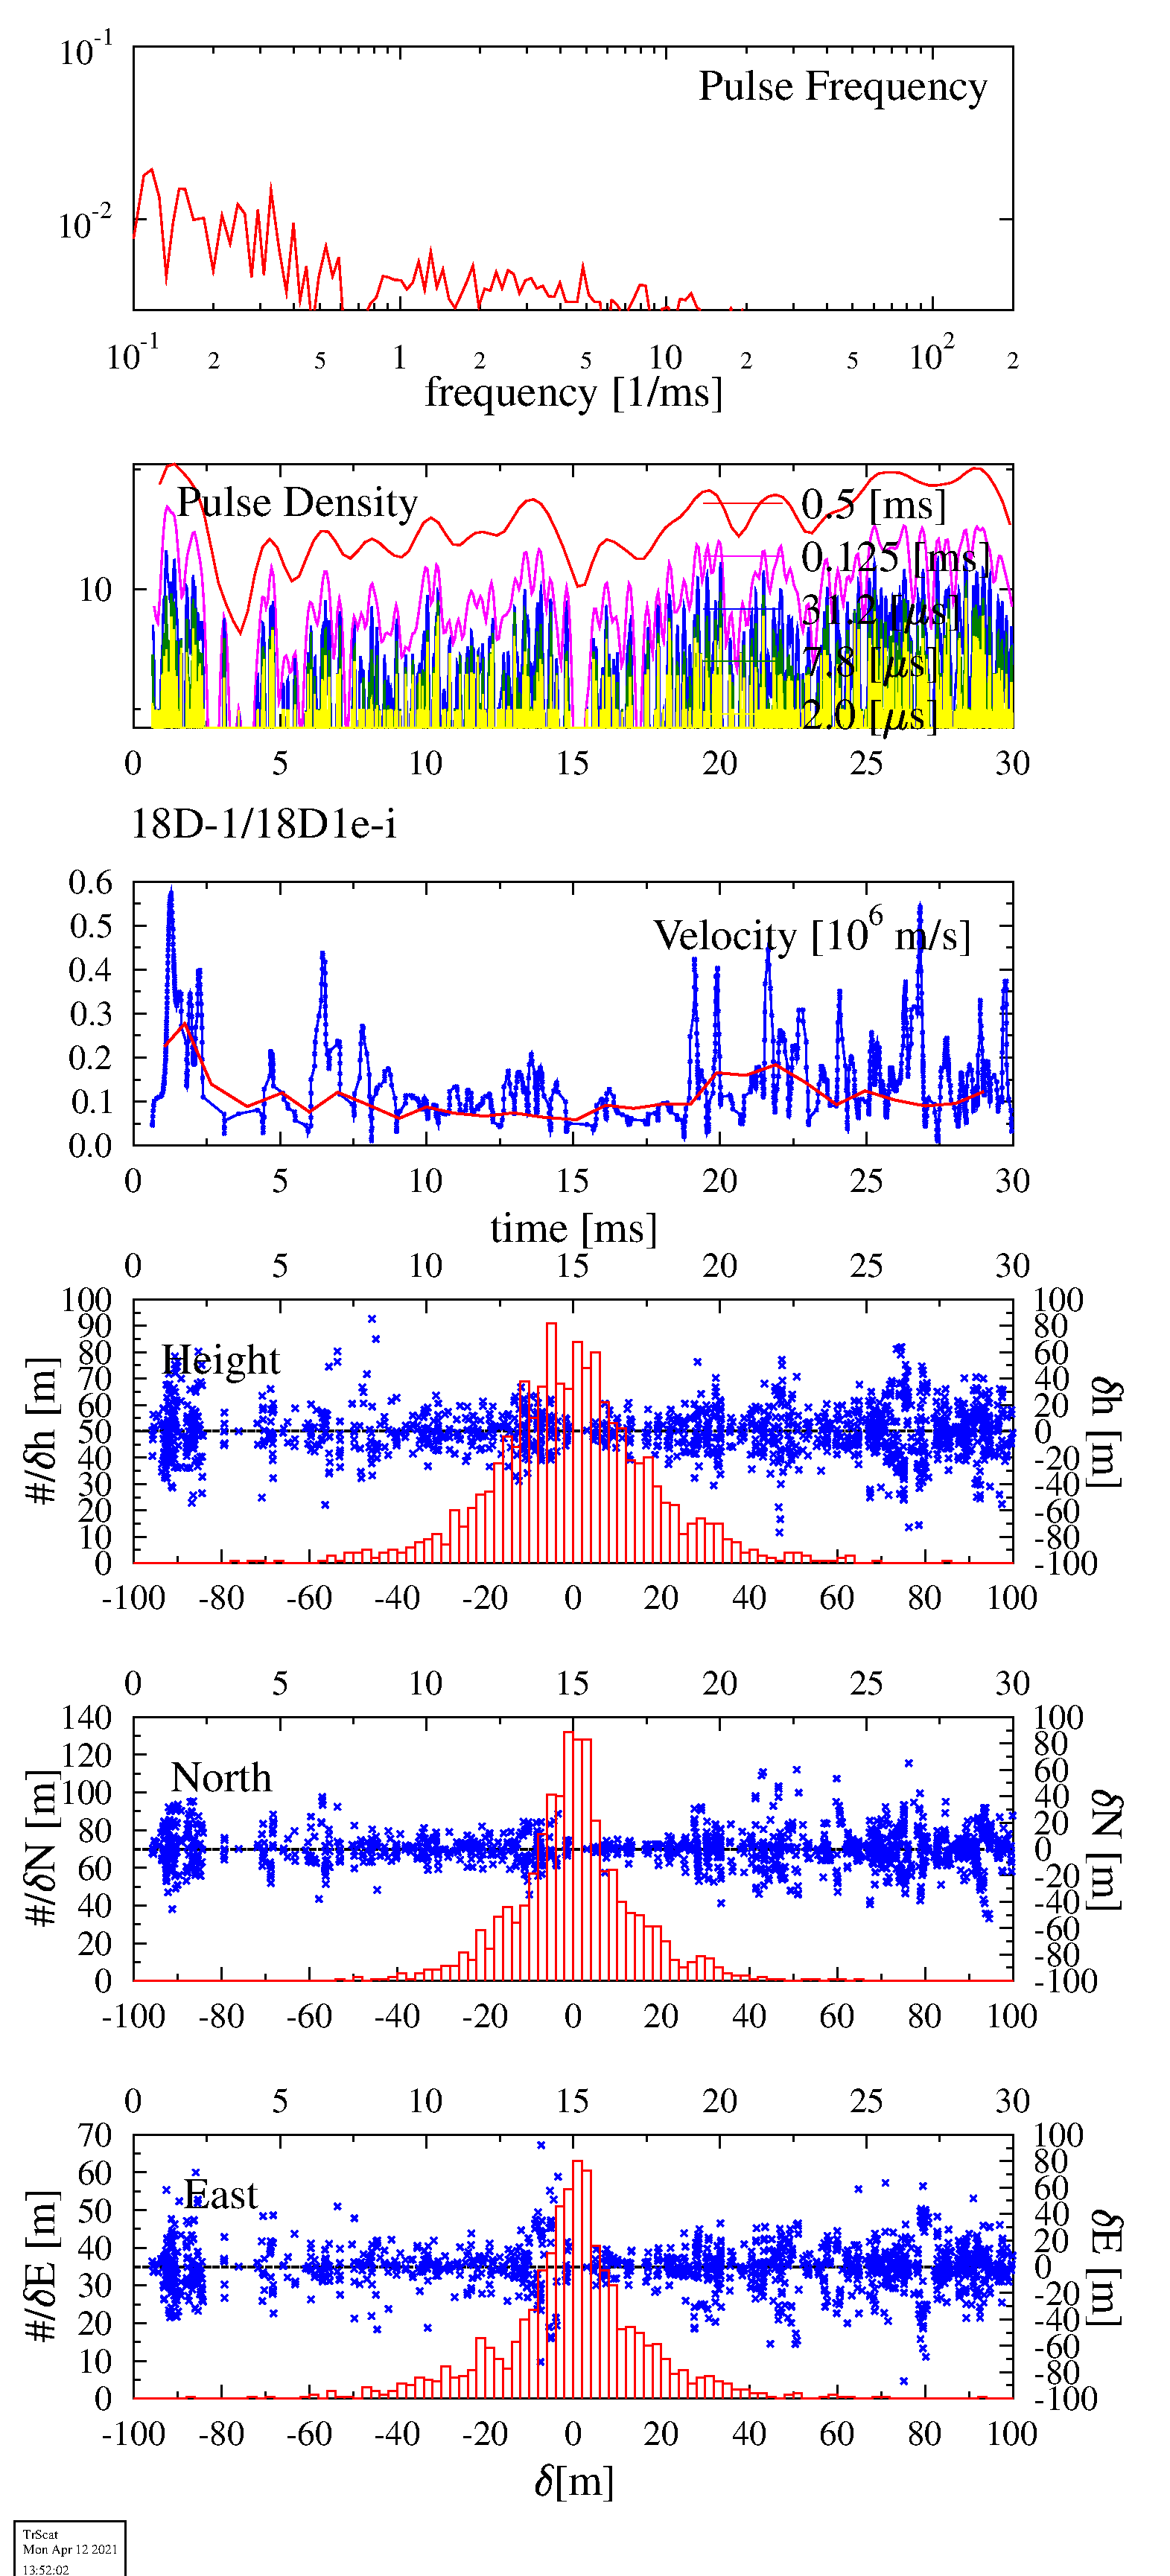
\includegraphics[ width=0.49\textwidth]{Figs/TrSc_18D1e-i} }
%\centering{\includegraphics[ bb=1.0cm 2.4cm 24.5cm 25.7cm,clip, width=0.49\textwidth]{../Figs/SE20A7-NPMx_1HIntfSpecSel} }
	\caption{Typical image for the Impulsive Imager when showing the statistics along a track.}	 \figlab{ImpulsiveTrack}
\end{figure}

If the 7th number on the second line in the input, ``FlashImage.in", is positive, a graph like \figref{ImpulsiveTrack} is made for each track. The second panel from the top shows the pulse density along the flash as function of time for various width of a gaussian smoothing function. The top panel shows the fourier decomposition of this plot. The third from the top gives the velocity along the track. The blue line for each source along the track, the red line for an average leader-tip location. The bottom three panels show the spread of the sources in the three directions from the propagating tip of the leader, in blue as a scatter plot v.s.\ time of the source (top and right scales), in red as a histogram (bottom and left scales).

For TRI-D based images a Principal Component analysis is performed on the direction of the polarization vector for each slice and a plot is make.

\subsection{Power spectrum}
Produces a power-law fit to source intensities, much like what was used in Ref.~\cite{Machado:2021, Scholten:2021-INL}

Some Generic options when using data from both imagers, with their default value:
\begin{enumerate*}
\item \verb! MaxAmplFitPercent= 0.1 !: Max amplitude fitted with modifies power law. (TRI-D only?)
\end{enumerate*}

The result is displayed in \figref{ImpulsiveImg} for the image of the flash for the selected area. The normalized pulse powers distributions $N(I)$ are fitted with a modified exponential,
\begin{equation}
N(I)= {\cal N}_e \,e^{-\alpha_e\,I-\gamma_e/I^2}\;, \eqlab{PowLaw}
\end{equation}
as well as with a modified powerlaw,
T\begin{equation}
N(I)= {\cal N} \,I^{-\alpha}  \,e^{-\gamma/I}\;, \eqlab{PowLaw}
\end{equation}
where $I$ is expressed in units of [GB]. The last factor, dependent on $\gamma$, suppresses the distribution at small amplitudes to good agreement with the data. The values for the fitted values for the normalization ${\cal N}$, the power $\alpha$, and the small-intensity suppression factor $\gamma$ are given in the output file (with extension .out).

The out file %\verb#'IntfrSrcSel.out'# looks like

\begin{linenumbers}
\tiny
\resetlinenumber
\begin{verbatim}
 ======================  Mx_d
 After file:files/IntfSpecPowMx_d.dat, SourcTotNr=          59
 Time span data=   343.94184999999999        343.94967000000003
Amplitudes (#=      59), max@ 198243.0, 5-pctile@********, 10-pctile@87401.70
Amplitude with   0.001pctile as included in fit @********
 $b *exp(-a*A-c/A^2); \chi^2=$  0.98,with  a,b,c=  0.0023 0.903E-05   0.00    ; nrm=  0.805E+05
 $b *A^-a *exp(-c/A); \chi^2=$  0.97,with  a,b,c=   4.023 0.156E+07   0.00    ; nrm=  0.805E+05
 $b *exp(-a*A-c/A^2); \chi^2=$  0.98,with  a,b,c= 0.2304E-020.9031E-05   0.00    ; nrm=   6.10      0.805E+05
 $b *A^-a *exp(-c/A); \chi^2=$  0.97,with  a,b,c=  4.023    0.1562E+07   0.00    ; nrm=   7.04      0.805E+05
 number of sources in plots:          59   1000.0000000000000      Mx_dIntfSpecSel
 ======================  End input
\end{verbatim}
\end{linenumbers}

Showing the number of points that fall within the plot boundary. A fit is made to the power spectrum for different functional dependencies and the resulting parameters are specified.

\subsection{Space-time correlation}

Produces the space-time correlation plots as used in Ref.~\cite{Wang:2023}

The calculation of TD correlators requires positive values for "Corr\_dD" and "Corr\_Dnr"
\begin{enumerate*}
\item \verb!Corr_dD !: Distance step size for time-distance correlator.
\item \verb!Corr_Dnr!: max. number of distance bins for time-distance correlator.
\item \verb!Corr_dtau=!: Time step size for time-distance correlator.
\end{enumerate*}


\clearpage 

\section{Compare Calibrations}\seclab{CompCal}

The purpose of \verb!"CompareCalibr.sh"! or  \verb!"CompareCalibr.bat"! is to list the differences between two calibration files stored in the folder \verb!"/Book"! of the main flash-working directory `FlashFolder'.

The file names to be processed are read from  \verb!"CompareCalibr.in"! looking like

\begin{linenumbers}
%\tiny
\resetlinenumber
\begin{verbatim}
"Calibrations202202060953.dat"
"Calibrations202202061011.dat"
\end{verbatim}
\end{linenumbers}

\subsection{Additional details}
none

\subsection{Figures and print-out}%\seclab{RFI-out}

No figure, print out file \verb!"CalComp.out"! looks like

\begin{linenumbers}
\tiny
\resetlinenumber
\begin{verbatim}
 Calibrations202202061011.dat minus Calibrations202202060953.dat in [ns]
 CS001 CS002 CS003 CS004 CS005 CS006 CS007 CS011 CS013 CS017 CS021 CS026 CS030 CS032 CS101 CS103 CS401 CS201 CS501 CS301 CS302 CS024 CS031 CS028
  0.06  0.00  0.02  0.03  0.03  0.00  0.02  0.04 -0.00  0.03 -0.00  0.03 -0.04  0.04 -0.03  0.03  0.03  0.06 -0.07  0.10  0.13  0.08 -0.01 -0.06
 RS106 RS205 RS208 RS305 RS306 RS307 RS310 RS406 RS407 RS409 RS503 RS508 RS509 RS210
  0.32  0.46  1.75  0.00  0.26  1.19  2.38 -0.65 -0.74  0.28  0.00 -1.05 -1.05  0.00
\end{verbatim}
\end{linenumbers}

and should be obvious.

\section{Interference Sources Select}\seclab{InterfSrc}

Note: This section in obsolete by now since the utility "InterfSrcSel" is superseded by "DataSelect" discussed in \secref{DataSelect}.

It is recommended to run the script \verb!"InterfSrcSel.sh"! using \verb!"InterfSrcSel.in"! as input to produce the plots that are zoomed in on the region of interest of the images made by the TRI-D imager, or to assemble the results of several TRI-D runs into a single image.

A typical input \verb!"InterfSrcSel.in"! resembles

\begin{linenumbers}
%\tiny
\resetlinenumber
\begin{verbatim}
&Parameters
 SMPowCut = 15e2 ! 5.e3
 AmpltPlot=10.
 MaxAmplFitPercent=0.001
 ZoomClip = .true.
 datafile=  "H99nw1",  "H99nw2"
 OutFileLabel="XYZ",
! xmin=-24.16 , xmax=-24.08, ymin=-10.25, ymax=-10.17, zmin=5.34, zmax=5.38  ! for NLa 37.10 37.6 -25.5 -25.25  5.35 5.8
!  tmin=606.552 , tmax=606.556
&End
xxxxxxxxxxxxxxxxxxxxxxxxxxxxx
\end{verbatim}
\end{linenumbers}

\begin{enumerate*}
\item[2] \verb!'SMPowCut = 15e2'!: Plot only those sources for which the intensity exceeds the specified limit.
\item[3] \verb#"AmpltPlot=10."#: The diameter of the largest symbols used in the plot. When zero or negative a fixed size dot will be used for all points, independent of their intensity.
\item[4] \verb!"! ZoomClip = .true."!: Only the points falling inside the plot boundary will be drawn.
\item[5] \verb#'datafile=  "H99nw1",  "H99nw2"'#: The \verb!"OutFileLabel="! from the different TRI-D runs for which the images have to be merged. This may also be just from a single run.
\item[6] \verb#'OutFileLabel="XYZ",'#: An additional label for the resulting plots, this in addition to the first entry in \verb#'datafile= '#.
\item[7] \verb#'! xmin=-24.16 , xmax=-24.08,'#: The boundaries of the plots will be taken from the first entry in \verb#'datafile= '# but will be overwritten if any of these settings is activated.
\end{enumerate*}

\subsection{Figures and print-out}%\seclab{RFI-out}

The produced .dat files are plain text files and contain some header lines with some general information followed by the specific data of the sources. The files have a format that is suitable for the plotting script \verb!"SourcesPlot.gle"!.

The out file \verb#'IntfrSrcSel.out'# looks like

\begin{linenumbers}
\tiny
\resetlinenumber
\begin{verbatim}
 ======================  Mx_d
 After file:files/IntfSpecPowMx_d.dat, SourcTotNr=          59
 Time span data=   343.94184999999999        343.94967000000003
Amplitudes (#=      59), max@ 198243.0, 5-pctile@********, 10-pctile@87401.70
Amplitude with   0.001pctile as included in fit @********
 $b *exp(-a*A-c/A^2); \chi^2=$  0.98,with  a,b,c=  0.0023 0.903E-05   0.00    ; nrm=  0.805E+05
 $b *A^-a *exp(-c/A); \chi^2=$  0.97,with  a,b,c=   4.023 0.156E+07   0.00    ; nrm=  0.805E+05
 $b *exp(-a*A-c/A^2); \chi^2=$  0.98,with  a,b,c= 0.2304E-020.9031E-05   0.00    ; nrm=   6.10      0.805E+05
 $b *A^-a *exp(-c/A); \chi^2=$  0.97,with  a,b,c=  4.023    0.1562E+07   0.00    ; nrm=   7.04      0.805E+05
 number of sources in plots:          59   1000.0000000000000      Mx_dIntfSpecSel
 ======================  End input
\end{verbatim}
\end{linenumbers}

Showing the number of points that fall within the plot boundary. A fit is made to the power spectrum for different functional dependencies and the resulting parameters are specified.

Two gle-scripts \verb#'%UtilDir%Intensity.gle'# and \verb#'%UtilDir%SourcesPlot.gle'# make the following plots.

\begin{figure}[h]
\setlength{\unitlength}{.48\textwidth} % .43\textwidth}
   \subfloat[Figure `IntfSpecSel']{ 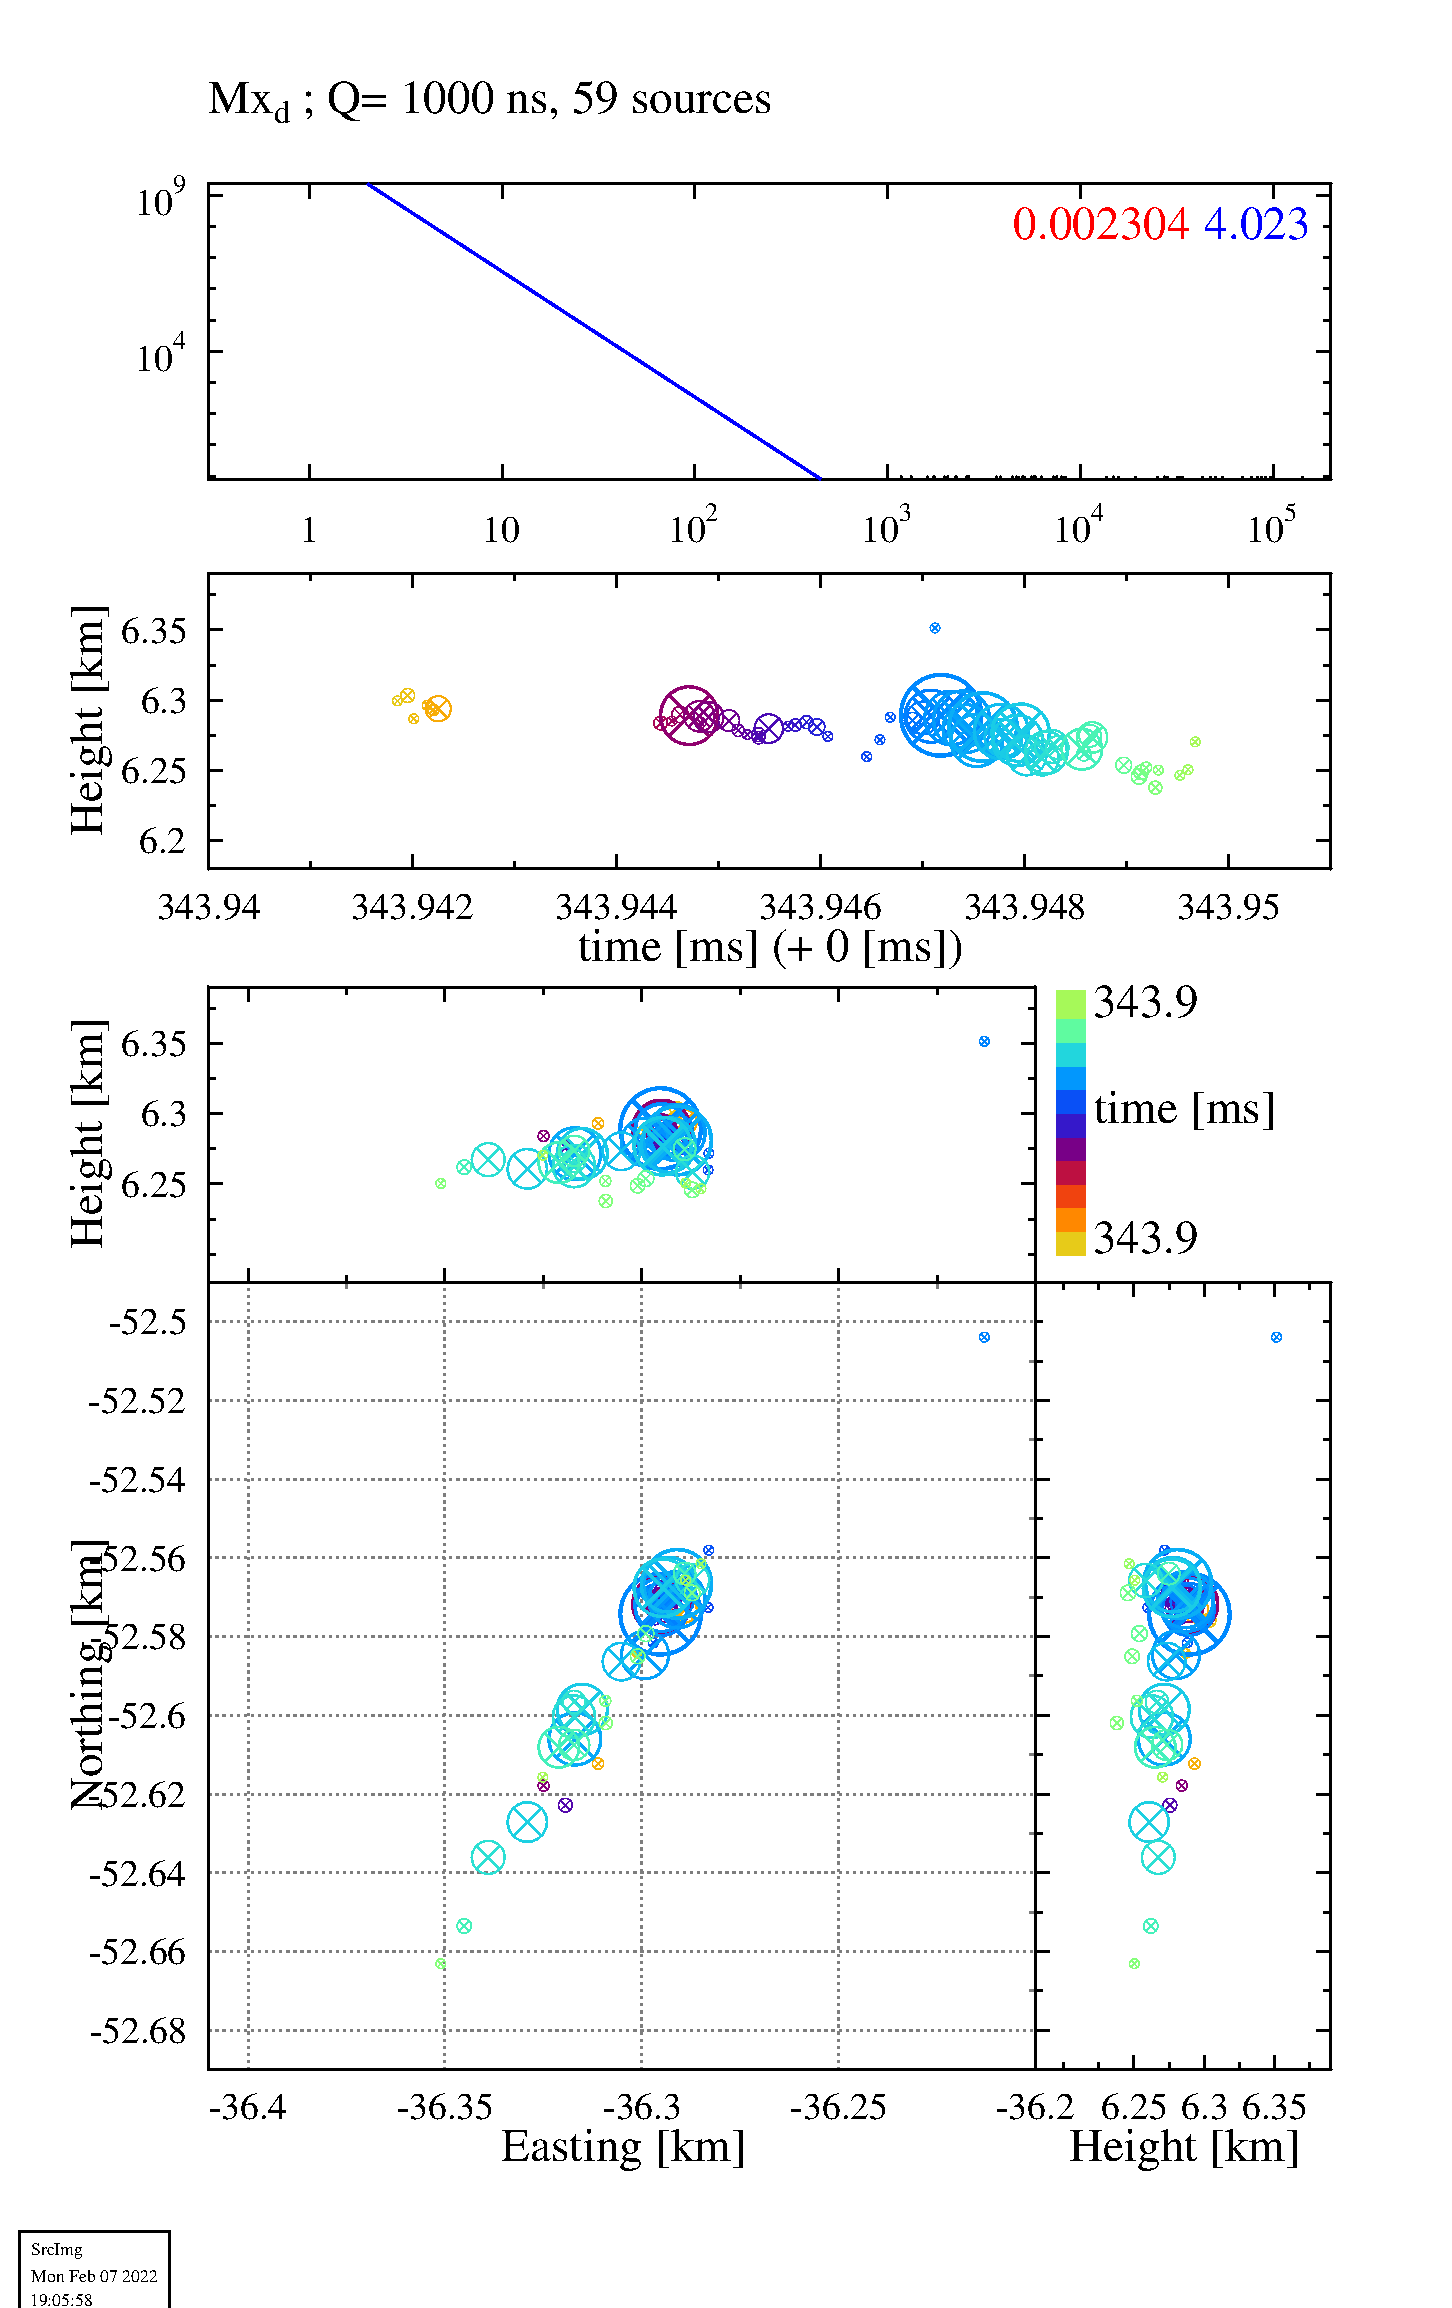
\includegraphics[width=\unitlength]{Figs/Mx_dIntfSpecSel}  \figlab{InterfSrc-Spec}}
   \subfloat[Figure `AmplFit']{ 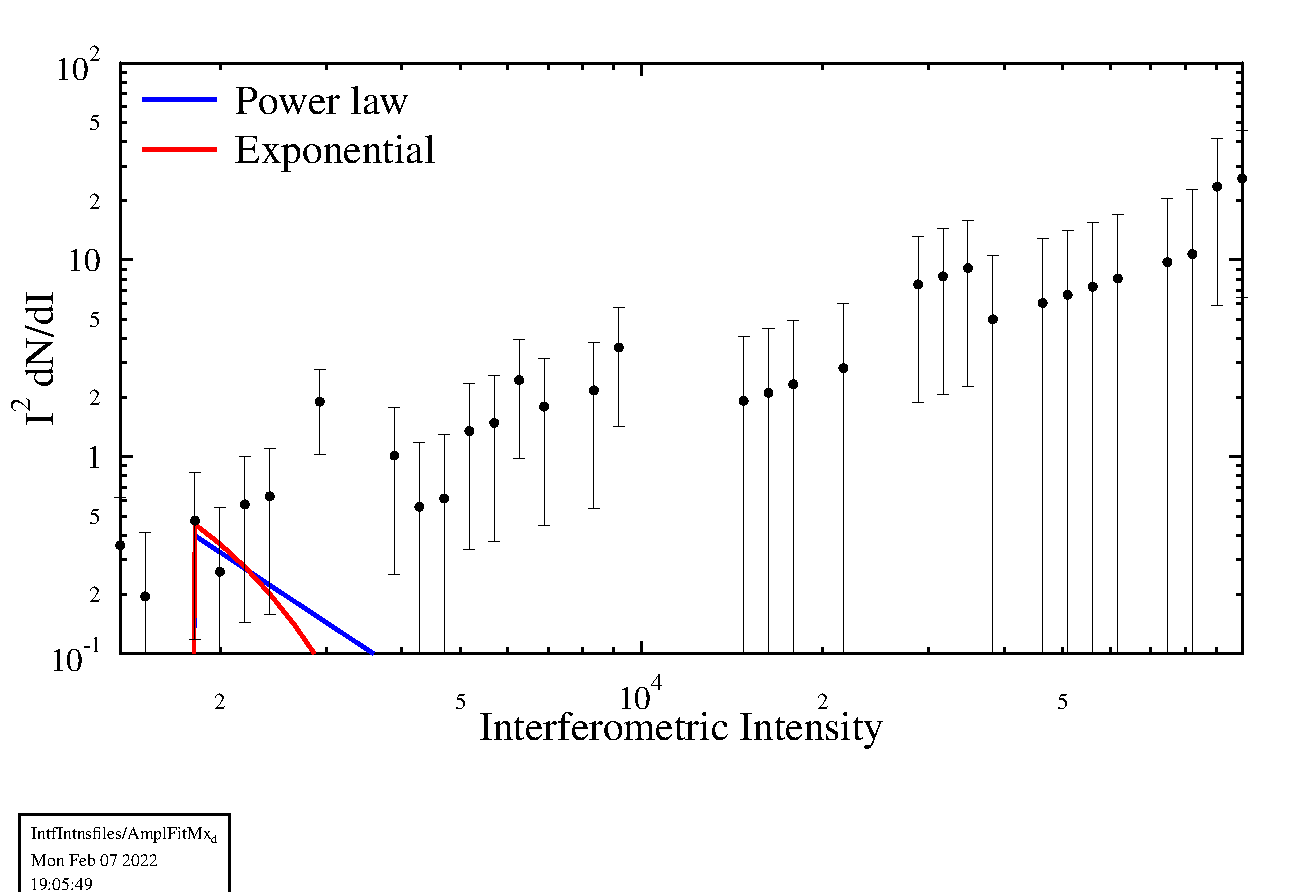
\includegraphics[width=\unitlength]{Figs/Mx_dAmplFit}  \figlab{InterfSrc-Ampl}}
	\caption{Top panel in \figref{InterfSrc-Spec} shows the intensity distribution of the sources and two fits (that obviously do not resemble the data for this case). The lower panels the usual way of plotting the sources where the size of the circles reflects the intensity.
\figref{InterfSrc-Ampl} displays an attempt to fit the pulse-strength distribution.}	 \figlab{InterfSrc}
\end{figure}

\clearpage


\section{Simulate}\seclab{Sim}

The purpose of \verb!"Simulate.sh"! or  \verb!"Simulate.bat"! is to simulate various source structures and text how these pass through the imager and has been used in~\cite{Scholten:2022}.

The file names to be processed are read from  \verb#`Simulate.in'# and \verb#`SimIntf.in'#  looking like

\begin{linenumbers}
%\tiny
\resetlinenumber
\begin{verbatim}
&Parameters
 Antennas="simulation/S1-1",
 Simulation="simulation/Discr"
 SrcNrMax = 1000
 NtSamples=1000
 TimingErr_ns = 1.
! FracGalacNoisePow=0.5
 OutFileLabel="tst"  , &end
  0.0  20.35,   18.65,    4.15,      -200.0 200. 300.       !  "Slant_500"
 Cloud 40. 10. 0.1 1000              ! 100% error                         !  cloud
  300.0  20.35,   18.65,    4.15,      -20.0 20. 30.       !  "Slant_50"
 Repeat 150 4         !  "ASync"
  0.0  20.35,   18.64,    4.15,      -300.0 300. 450.       !
\end{verbatim}
\end{linenumbers}

\begin{enumerate*}
\item[2] \verb#' Antennas="simulation/S1-1",'#: The information on the positions of the antennas is read from these files in the "files" subfolder. These files are most efficiently created with the `SelectData' option as discussed in \secref{SelDat}. Note that exclusively the antenna positions are used.
\item[3] \verb#' Simulation="simulation/Discr" '#:  The place in the "files" folder where the simulation results are written.
\item[4] \verb#' SrcNrMax = 1000'#:  The maximum number of single point sources that can be simulated.
\item[4] \verb#' NtSamples=1000'#:  The maximum length (in samples) of the time trace. The minimal number is 400 samples and will be rounded up to a power of 2.
\item[5] \verb#' TimingErr_ns = 1.'#:  The standard deviation of the calibration-timing-error that are assigned to each antenna.
\item[6] \verb#'! FracGalacNoisePow=0.5'#: relative fraction of galactic noise to the total noise. Galactic noise has a 1/frequency spectrum, while instrumental noise is taken to be flat. In actual calculations this hardly matters.
\item[7] \verb#' OutFileLabel="tst",'#:  Additional label for results files.
\item[8] \verb#'   0.0  20.35,   18.65,    4.15,      -200.0 200. 300.   '#:  A point source is put at time=0 [samples] and position (N,E,h)=(20.35, 18.65, 4.15)~km with dipole strength in direction (N,E,h)=(-200.0 200. 300.). A dipole strength of 1. will show with the same amplitude as the noise when the source is placed at a favorable angle at a distance of 1~km from the antenna. There may be many lines like this one. Note that the times of the produced traces is shifted such as to put the first source at sample 200 for the reference antenna.
\item[9] \verb#' Cloud 40. 10. 0.1 1000  '#: Put a cloud of 1000 single point-sources as specified in the following line with a standard deviation of spread in time of 40~[samples], in 3D-position of 10~[m], and in 3D-polarization of 0.1
\item[11] \verb#' Repeat 150 4'#:  Place 4 sources with the same properties at the same position at time intervals of 150 samples.
\end{enumerate*}

\subsection{Output files and print-out}%\seclab{RFI-out}

The generated output files have a very similar structure as those discussed in \secref{SelDat-out}.
The files will be used as input when running the impulsive of the TRI-D imager with option \verb!`Simulation="simulation/Discr" '!
The traces are constructed starting 200 samples before the time of the first source (at the correct time calculated from the position of the first source and the position of the antenna).
Thus, is the first source is at sample 0, the interferometry could be run with  $t=-0.011$ and sample offset 2000 to have the beginning of the investigated trace at the beginning of the generated background. Note that the first source may be 'fake' and have zero intensity.

\subsection{Power calibration}\seclab{PowerCal}

\subsubsection{Pulse}
Starting definitions:
\\$M_{e/o}^a[t] = $ time trace as results from reading the data in ant-read.f90, i.e. filtered and normalized, for one antenna labeled by $a$. $N_{e/o}$ are the corresponding averaged norm factors for even and odd antennas with on average $N_{e/o}=1/{\rm NormEvenOdd}$ with ${\rm NormEvenOdd}=100.$ and are canceled in reading data.
\\$D^a_p[t] =$ time trace used in the TRI-D fitting of the dipole moments. Here $a$ is the label of an antenna pair and $p$ stands for azimuth or zenithal polarization of the field seen by the antenna.
\\${\cal F}$ labels the fourier transform from time to frequency, $J[\theta,\phi](\nu)$ the antenna function transforming from $\nu_p$ (polarization direction) to $\nu_{e/o}$ antenna direction.
\\$G_0[\nu] =\sqrt{(\sum_p\sum_{e/o} J^2[0,0](\nu))/\Delta_\nu}$ is the antenna gain for the vertical direction, where $\Delta_\nu$ is the total bandwidth, typically 30--80~MHz.
Now
\beq
D^a_p[t] =  {\cal F}^{-1}\left(  G_0[\nu]\, J^{-1}\left( N_{e/o}\,{\cal F}(M_{e/o}[t]) \right) \right) \;,
\eeq
omitting the obvious antenna label and noting that this may be complex. This is fitted by the TRI-D fitter (per time sample) to
\beq
{\rm TRI}^a_p[t]=  \vec{p} \cdot \vec{I}[t] /R \;,
\eeq
where $R$ is the antenna-source distance.  $\vec{I}[t]$ is used for calculating the stokes parameters from $Stokes=(1/N_t)\sum_t \vec{I}^\dagger \vec{I}$ where $N_t$ is the number of time samples.

In the simulations we define in addition:
\\$\delta[\nu] = {\cal F} \delta[t]$ where $\delta[t]$ is a time trace equal to zero except for one sample where it equals unity.
\\${\cal I}[t] = {\cal F}^{-1} G_0[\nu] \, \delta[\nu]$ is the impulse response for a source that is vertically overhead to an antenna.
\\$\vec{I}_s = $ source dipole vector. $N_I=$ norm factor relatively arbitrarily set to $N_I=20 \sqrt{14} /TotalGain$
The simulated time trace, $S^a_{e/o}[t]$, that is written to file, is
\beq
S^a_{e/o}[t] = \frac{1}{N_{e/o}} \,N_I\, \Re {\cal F}^{-1}\left( J[\theta,\phi] \left( \vec{p} \cdot \vec{I}_s \right) \delta[\nu] /R \right)
\eeq
where the viewing angles to the source, $[\theta,\phi]$, depend on antenna number $a$ and where on reading-in this trace using the simulation option $N_{e/o}=1/{\rm NormEvenOdd}$ is set, equal to the average when reading real data.

When pulling the simulated data through the TRI-D procedure for the data we obtain
\beq
D^S_p[t] = N_I\,{\cal F}^{-1}\left(  G_0[\nu]\times \left( \vec{p} \cdot \vec{I}_s \right) \delta[\nu] /R \right) \;,
\eeq
using $G_0[\nu] J^{-1}\,J =G_0[\nu] \delta_{p,p'}$ where the factor $G_0$ prevents dividing by zero, and ${\cal F}^{-1} {\cal F}=1$.
To numerically agree with the result from the TRI-D imager we thus obtain
\beq
\vec{I}[t] = N_I\,{\cal F}^{-1}\left(  G_0[\nu]\times \delta[\nu]  \right)\, \vec{I}_s \;.
\eeq
Since $St_I=(1/N_t)\,\sum_t |\vec{I}[t]|^2$ we obtain by putting $|\vec{I}_s |^2=St_I$
\beq
St_I = |\vec{I}_s|^2 \frac{N_I^2}{N_t} \sum_t \left| {\cal F}^{-1}\left(  G_0[\nu]\times \delta[\nu]  \right) \right|^2 \;,
\eeq
as the conversion factor between the input values for the dipole moments in the simulation program to the [gb] units used in TRI-D.

The background power level in the simulation program is set to the same value as used in the LOFLI code.

The results for a source in the simulation code are:
\begin{verbatim}
TRI-D re-norm 0.0214, Intensity at window edge= 0.0018% of peak, TotalGain=   17.869, slicing window IntfSmoothWin= 50
   #  Dt[smpl]   t[smpl]     (N,E,h) [km]                   Ampl(N,E,h)               I123_TRI-D
   1     0.00      0.0     -0.4160    0.5590   45.0000     -0.10    0.00    0.00          0.00
   2  1010.06   1010.0     -0.4260    0.5590   45.0000   2000.10    0.00    0.00       1824.43
   gives
Station=  1        3 CS003 uses 4 antenna pairs. Start time=   0.14916[ms]
 * background power/sample=  0.99984436946070021        1.0122509563864033
 * total power in background=   4095.3625373110281        4146.1799173587078
 * power in sources only:   27196.887091213786        26836.486063132907
 * total power, backgr + sources=   31292.249628524776        30982.665980491667
 Ave background power (all antennas)=  1.   1.006  N_even=N_odd= 162  Tracelength= 4096 samples
\end{verbatim}
\Omit{  -------------------- Omitted
from which we deduce that a source of $1824.43$~[gb] over a slice of $\Delta t=250$~ns (50 samples), straight overhead and transversely polarized, deposits an total energy of $27,016/4,096=6.6$ times that deposited by noise as seen by LOFAR after amplifiers over a time span of $4,096\times 5=20.48$~$\mu$s.
The noise of the LOFAR antenna corresponds to $P_{gb,K}=1.3\times 10^{-14}$~W/MHz Galactic background and the total background measured (if due only to gb) would correspond to a flux of $P_{n,K}=2.2\times 10^{-14}$~W/MHz (see discussion in \secref{SimBckgr}).
The total energy deposited thus corresponds to $E_a(D)=6.6\times 2.2\times 10^{-14} \times 20.48\times 10^{-6}=3\times 10^{-18}$~J/MHz (note different units).
A source emitting a short pulse with a power of $E_s$~[J/MHz] (transverse) vertically above an antenna $a$ at a distance of 45km ($D^2=2.03\times 10^3$~km$^2$) will deposit a pulse with energy $E_a$ obeying
\beq
E_s=0.5\times 4\pi \frac{D^2}{A_a} \times E_a \;J/MHz
\eeq
where the first factor $0.5\times 4\pi$ is due to the integration of the dipole intensity over solid angle and the effective area of the antenna is taken equal to $A_a=\lambda^2/4=25/4=6.25$~m$^2$.
Putting factors together we get that a source with strength $St_I$~[gb] thus emits a total energy of
\bea
E_s &=& 2\pi \frac{D^2}{A_a} \times \frac{St_I\times \Delta t}{1824.43\,[gb]\times 250\,[ns]} \left(\frac{45\,[km]}{D}\right)^2 \times 3\times 10^{-18}\,[J/MHz] \nonumber \\
&=&  2\pi \frac{45^2\,[km]^2}{A_a} \frac{1}{1824.43\times 2.50} \times 3\times 10^{-18} \times \frac{St_I\times \Delta t}{1\,[gb]\times 100\,[ns]}\, [J/MHz] \nonumber \\
&=&  2\pi \times 2.03 \times 10^9 \frac{1}{1824.43\times 2.50} \frac{1\,m^2}{A_a}\times 3\times 10^{-18} \times \frac{St_I\times \Delta t}{1\,[gb]\times 100\,[ns]}\, [J/MHz]  \nonumber \\
&=& \frac{1\,m^2}{A_a} 8.4 \times 10^{-12} \times \frac{St_I\times \Delta t}{1\,[gb]\times 100\,[ns]}\, [J/MHz]
\eea
putting the antenna effective area of $A_a(60MHz,\theta=0,\phi=0)=1$~m$^2$ as used by Katie in making her Figure 5 where the true area is included in the gain factor.

\subsubsection{revised}\seclab{rev-pulse}
} % --------------------end Omit

from which we deduce that a source of $1824.43$~[gb] over a slice of $\Delta t=250$~ns (50 samples), straight overhead and transversely polarized, deposits an total energy of $27,016/4,096=6.6$ times that deposited by noise as seen by LOFAR, after amplifiers, over a time span of $4,096\times 5\times 10^{-9}=20.48 \times 10^{-6}$~s.

The noise of the LOFAR antenna corresponds to $P_{gb,K}=1.3\times 10^{-14}$~W/MHz Galactic background and the total background measured (if due only to gb) would correspond to a flux of $P_{n,K}=2.2\times 10^{-14}$~W/MHz (see discussion in \secref{SimBckgr}).
The total energy deposited thus corresponds to $E_a(D)=6.6\times 2.2\times 10^{-14} \times 20.48\times 10^{-6}=3\times 10^{-18}$~J/MHz (note units).

A source emitting a short pulse with a power of $E_s$~[J/MHz] (transverse) vertically above an antenna $a$ at a distance of 45km ($D^2=2.03\times 10^3$~km$^2$) will deposit a pulse with energy $E_a$ obeying
\beq
E_s=8\pi/3 \frac{D^2}{A_a} \times E_a \;J/MHz
\eeq
where the first factor $8\pi/3$ is due to the integration of the dipole intensity over solid angle ( the electric field is proportional to sinus and the power the square of the E field, giving $$\int \sin^2(\theta) d[\cos(\theta)] d\phi=2\pi \int_{-1}^{+1} (1-x^2)\,dx=4\pi(1-1/3)=8\pi/3$$). The effective area of the antenna is often taken equal to $A_a=\lambda^2/4=25/4=6.25$~m$^2$, however, Katie used in making her Figure 5, an antenna effective area of $A_a(60MHz,\theta=0,\phi=0)=1$~m$^2$ where the true area is included in the gain factor.
Putting factors together we get that a source with strength $St_I$~[gb] thus emits a total energy of
\bea
E_s &=& 8\pi/3 \frac{D^2}{A_a} \times \frac{St_I\times \Delta t}{1824.43\,[gb]\times 250\,[ns]} \left(\frac{45\,[km]}{D}\right)^2 \times 3\times 10^{-18}\,[J/MHz] \nonumber \\
&=& 8\pi \frac{45^2\,[km]^2}{A_a} \frac{1}{1824.43\times 2.50} \times 10^{-18} \times \frac{St_I\times \Delta t}{1\,[gb]\times 100\,[ns]}\, [J/MHz] \nonumber \\
&=& 8\pi \times 2.03 \times 10^9 \frac{1}{1824.43\times 2.50} \times 10^{-18} \times \frac{St_I\times \Delta t}{1\,[gb]\times 100\,[ns]}\, [J/MHz]  \nonumber \\
&=&  1.1 \times 10^{-11} \times \frac{St_I}{[gb]} \times \frac{\Delta t}{100\,[ns]}\, [J/MHz]
\eea

\Omit{
\subsubsection{Background-Old}\seclab{SimBckgr-Old}
The brightness temperature of radiation is given by $T_b = (\lambda^2 / 2k)^{-1} I_\nu$.

 ``The Spectrum of the Radio Background Between 13 and 404 MHz'',
A.H.\ Bridle, J.E.\ Baldwin:%https://doi.org/10.1093/mnras/136.2.219
\\Fig10 from~\cite{Bridle:1967}: Brightness $ @60MHz=2.7\times 10^{-21}$~W/m$^2$/Hz/Sr (radiation coming from the North pole).
\\Integrate over the sky as seen by LOFAR (calculation gives Sr=2.3) this gives the energy flux for a LOFAR antenna ($A=1 m^2$ and at 60~MHz) $P_{gb,O}=2.7*2.3\times 10^{-21}$~W/Hz$=6.2\times 10^{-21}$~W/Hz.
\\Assuming the instrumental noise is about the same as the galactic background gives $P_{n,O}=1.24\times 10^{-14}$~W/MHz, however, most of the intensity in $P_{gb}$ comes from the Galactic disk at the equator and the North pole is somewhere in the halo. The mean is thus larger than the value at the North pole which is why Katie's numbers for $P_{gb,K}=1.3\times 10^{-14}$~W/MHz, obtained from an honest integration over sky angle \figref{Katie-Fig}, are larger than Olaf's value $P_{gb,O}=6.2\times 10^{-15}$~W/MHz. Note that $P_{gb,K}$ should depend on siderial time, see~\cite{Mulrey:2019}.


\begin{figure}[th]
\centering{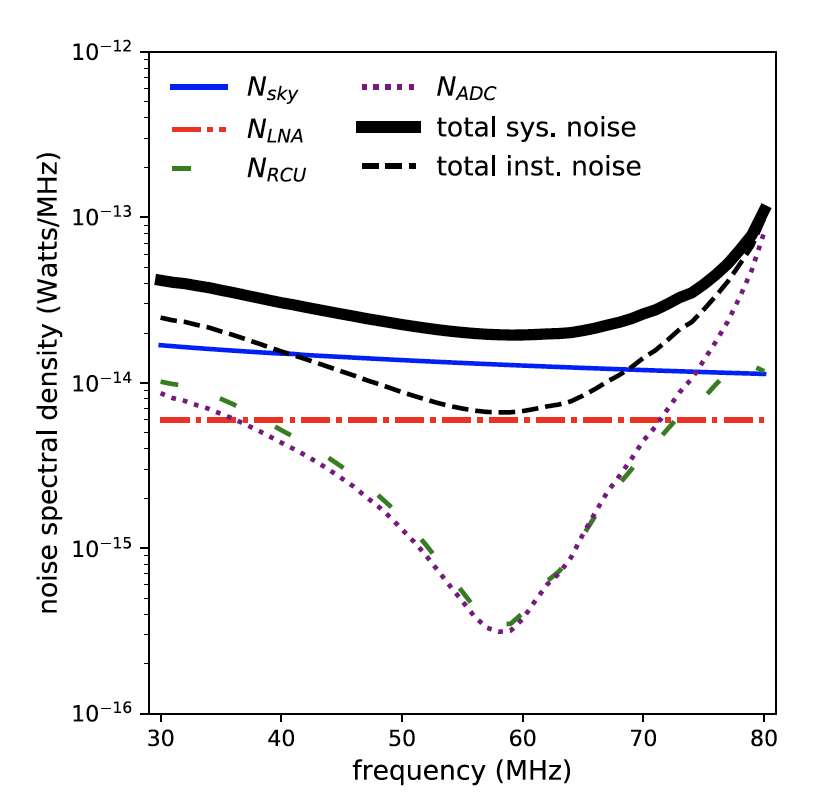
\includegraphics[width=0.44\textwidth]{Figs/LOFAR-antennaNoise,Katie2023-01-30} }
\centering{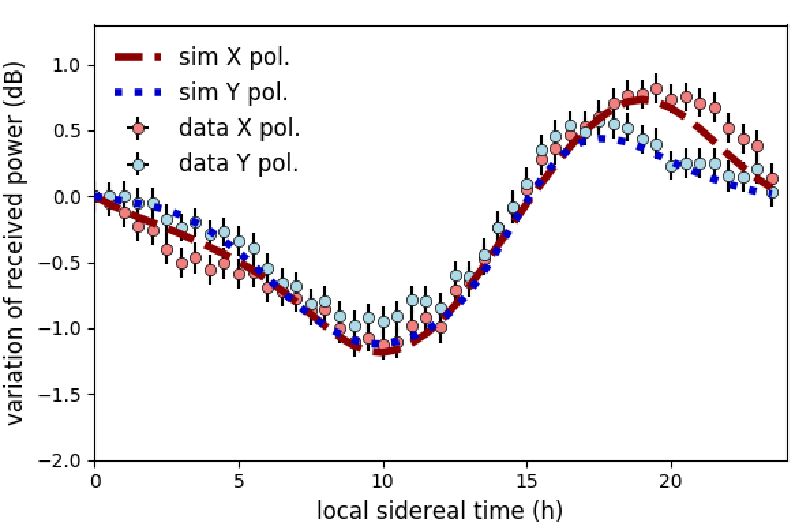
\includegraphics[width=0.54\textwidth]{Figs/KatieFig4Right} }
%\centering{\includegraphics[ bb=1.0cm 2.4cm 24.5cm 25.7cm,clip, width=0.49\textwidth]{../Figs/SE20A7-NPMx_1HIntfSpecSel} }
	\caption{Left: contribution to the noise level for a LOFAR LBA antenna where the antenna-gain has been unfolded. Right: variation of background with siderial time (1~dB=factor 1.26, 3~dB=factor 2, 10~dB=factor 10). Figures 5 and 4-right (Katie Mulrey, January 30, 2023) from \cite{Mulrey:2019}.}	 \figlab{Katie-Fig}
\end{figure}

\figref{Katie-Fig} shows the different contributions to the noise level after unfolding the antenna gain where the galactic noise is integrated over angle folding in the angle dependent antenna gain (normalized to zenith angle). This shows that the number for the total noise level should rather be $P_{n,K}=2.2\times 10^{-14}$~W/MHz when averaged over 30 -- 80~MHz. Note that in averaging over this frequency interval a frequency-weighting, proportional to the antenna gain, should be taken into account.

A source with intensity $St_I$~gb over a slice of duration $\Delta_t$ thus emits a total energy/MHz of
\\$F=0.5\times 4\pi D^2 \times St_I \frac{1\times 10^3}{D^2}\times 1.24\times 10^{-14}\times\frac{\Delta_t}{100ns}\times 10^{-7}$~J/MHz
\\where the first factor $0.5\times 4\pi$ is due to the integration of the dipole intensity over solid angle. Since the electric field is proportional to sinus and the power the square of the E field, this should have been $$\int \sin^2(\theta) d[\cos(\theta)] d\phi=2\pi \int_{-1}^{+1} (1-x^2)\,dx=4\pi(1-1/3)=8\pi/3$$, i.e.\ an extra factor $4/3$ that is not yet included in the following. Reducing this gives
\\$F=2\pi  \times St_I  \times 1.24\times 10^{-18}\times\frac{\Delta_t}{100ns} $~J/MHz


 This yields
$F_O=0.88 \times St_I\times\frac{\Delta_t}{100ns} \times 10^{-17} $~J/MHz $\approx St_I\times\frac{\Delta_t}{100ns} \times 10^{-5} $~pJ/MHz since pico$=10^{-12}$. An additional factor $10^6$ needs to be added because the effective area of the antenna is 1~m$^2$ and not 1~km$^2$

Using Katie's number for the background, \figref{Katie-Fig}, we get $F_K=0.88 (2.2/1.24) \times St_I \times \frac{\Delta_t}{100ns} \times 10^{-17} $~J/MHz $\approx 1.8 \times St_I \times \frac{\Delta_t}{100ns} \times 10^{-5} $~pJ/MHz

The background intensity for a tesseract depends on the distance to the core (increases with the square of the distance) and the number of antennas. The latter is difficult to quantify as this will depend on the intensity they receive as compared to the core, but roughly proportional to their number. The intensity of the brightest background source will increase with the number of voxels in the image cube and should decrease (slightly) with the duration of a slice. For a tesseract at $D^2=2\times 10^3$~km$^2$ and slice of $\Delta_t=100$~ns vertically above the core we obtain for the background noise level $I^n \approx 0.2$~gb. However, the sum of the two transverse components give only $I_{\perp}^n \approx 0.01$~gb. It is seen that for these distances the transverse scales with distance as expected, but the longitudinal intensity tends to diverge for large distances.

The Earth rotation angle (ERA), kind of the same as siderial time, measured in radians, is related to UT1 by a simple linear relation:[3]
\beq  \theta (t_{U})=2\pi (0.779\,057\,273\,2640+1.002\,737\,811\,911\,354\,48\cdot t_{U})
\eeq
where $t_U$ is the Julian UT1 date (JD) minus 2451545.0, that is, 12:00 (midday) Terrestrial Time of January 1, 2000, Unix Timestamp = 946728000. (Note that this differed from 12h UTC on that day by around a minute.)
Katie:  UTC=946728000 gives an LST=19.2 i.e. LST = ERA-.779+.2 = ERA-.58
} % end Omit

\subsubsection{Background}\seclab{SimBckgr}

A dirty guestimate of the background intensity is obtained from the brightness temperature of radiation is given by $T_b = (\lambda^2 / 2k)^{-1} I_\nu$.
Using  ``The Spectrum of the Radio Background Between 13 and 404 MHz'',
A.H.\ Bridle, J.E.\ Baldwin:%https://doi.org/10.1093/mnras/136.2.219
\\Ref~\cite{Bridle:1967}, Fig 10 gives: Brightness $ @60MHz=2.7\times 10^{-21}$~W/m$^2$/Hz/Sr (radiation coming from the North pole).
\\Integrate over the sky as seen by LOFAR (calculation gives Sr=2.3) this gives the energy flux for a LOFAR antenna ($A=1 m^2$ and at 60~MHz) $P_{gb,O}=2.7*2.3\times 10^{-21}$~W/Hz$=6.2\times 10^{-21}$~W/Hz.
\\Assuming the instrumental noise is about the same as the galactic background gives $P_{n,O}=1.24\times 10^{-14}$~W/MHz, however, most of the intensity in $P_{gb}$ comes from the Galactic disk at the equator and the North pole is somewhere in the halo. The mean is thus larger than the value at the North pole which is why Katie's numbers for $P_{gb,K}=1.3\times 10^{-14}$~W/MHz, obtained from an honest integration over sky angle \figref{Katie-Fig}, are larger than Olaf's value $P_{gb,O}=6.2\times 10^{-15}$~W/MHz. Note that $P_{gb,K}$ should depend on siderial time, see~\cite{Mulrey:2019}.


\begin{figure}[th]
\centering{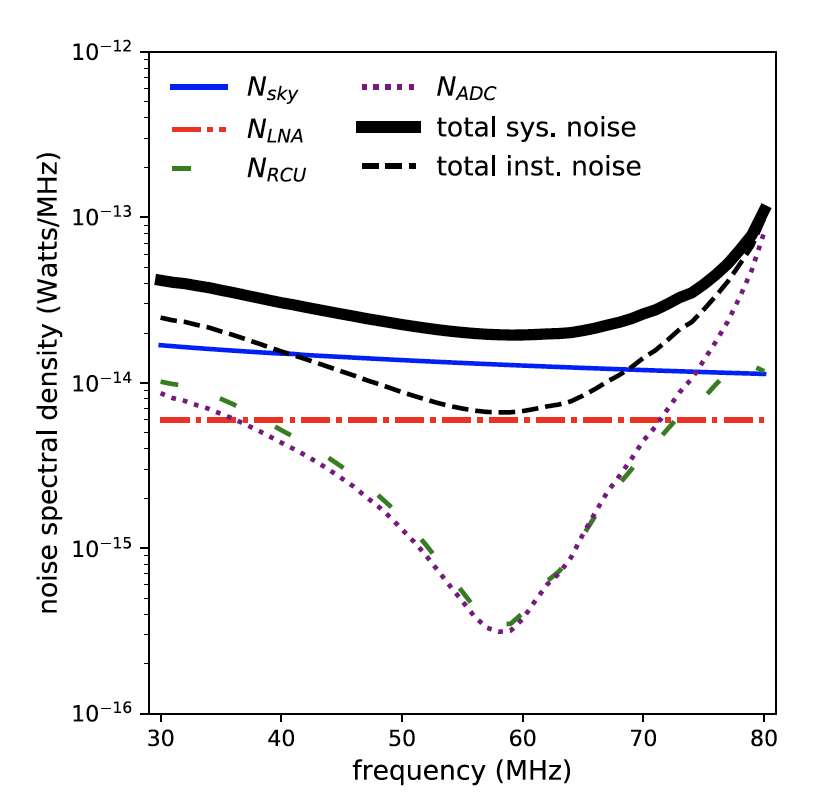
\includegraphics[width=0.44\textwidth]{Figs/LOFAR-antennaNoise,Katie2023-01-30} }
\centering{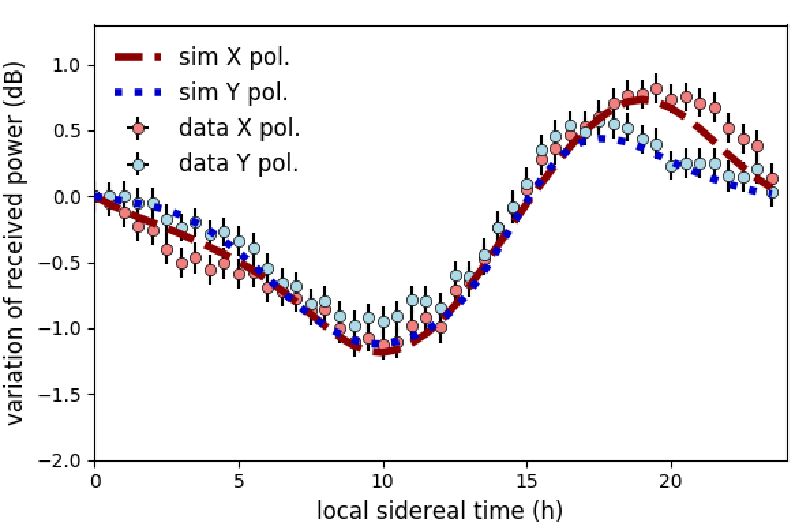
\includegraphics[width=0.54\textwidth]{Figs/KatieFig4Right} }
%\centering{\includegraphics[ bb=1.0cm 2.4cm 24.5cm 25.7cm,clip, width=0.49\textwidth]{../Figs/SE20A7-NPMx_1HIntfSpecSel} }
	\caption{Left: contribution to the noise level for a LOFAR LBA antenna where the antenna-gain has been unfolded. Right: variation of background with siderial time (1~dB=factor 1.26, 3~dB=factor 2, 10~dB=factor 10). Figures 5 and 4-right (Katie Mulrey, January 30, 2023) from \cite{Mulrey:2019}.}	 \figlab{Katie-Fig}
\end{figure}

More accurately \figref{Katie-Fig} shows the different contributions to the noise level after unfolding the antenna gain where the galactic noise is integrated over angle folding in the angle dependent antenna gain (normalized to zenith angle). This shows that the number for the total noise level should rather be $P_{n,K}=2.2\times 10^{-14}$~W/MHz when averaged over 30 -- 80~MHz. Note that in averaging over this frequency interval a frequency-weighting, proportional to the antenna gain, should be taken into account.


The Earth rotation angle (ERA), kind of the same as siderial time, measured in radians, is related to UT1 by a simple linear relation:[3]
\beq  \theta (t_{U})=2\pi (0.779\,057\,273\,2640+1.002\,737\,811\,911\,354\,48\cdot t_{U})
\eeq
where $t_U$ is the Julian UT1 date (JD) minus 2451545.0, that is, 12:00 (midday) Terrestrial Time of January 1, 2000, Unix Timestamp = 946728000. (Note that this differed from 12h UTC on that day by around a minute.)
Katie:  UTC=946728000 gives an LST=19.2 i.e. LST = ERA-.779+.2 = ERA-.58


\chapter{Some not well assorted formulas (theory)}\seclab{theory}
\section{E-field Interferometric imaging}\seclab{E_Intf}

This chapter is a rather random put together of various more background material that certainly could use a better organization.

\subsection{Method of Time Resolved Interferometric 3D Imaging}\seclab{TRID}

This section is adapted from the draft of the manuscript ``Time resolved 3Dinterferometric imaging of a section of a negative leader with LOFAR"

The basic implementation of beam-forming imaging is relatively straightforward. The part of the atmosphere where the lightning is to be imaged is divided up in voxels. For each voxel the time traces of the antennas are summed while accounting for the difference in travel time from this voxel to each antenna. This yields for each voxel a time trace which is the coherent sum of all antennas, as discussed in \secref{Vox}. Adding the traces for the different voxels is always performed for a fixed time span in one particular `reference' antenna, usually one from the core of LOFAR. Thus we can find the source location of a particular structure seen in the trace of the reference antenna.

The time trace of each voxel is cut in slices of a fixed duration. The intensity is determined for all slices resulting in many voxelated intensity profile, one such profile for each time slice corresponding to a fixed time slice in the reference antenna, much like what is shown in \figref{B-NLa-166} but for much shorter time spans.
The length of the time slices determines our final time resolution since any detail within a slice is summed over.
For each time slice the maximum of this voxelated intensity profile is determined and used as the source location, as discussed in more detail in \secref{Max}. Plotting the position of all sources will result in the beam-formed (or interferometric) image of a segment of the flash in space and time. In the following the different steps involved in this procedure are discussed in more detail.

The main selling points of LOFAR are that we  can reach 1) a time resolution of 100~ns, the pulse response width as determined by the band width (30-80~MHz) 2) a spatial resolution of the order of 1~m, determined by the time calibration (order 1~ns) and the antenna baselines (up to 100~km), 3) a sensitivity of two orders of magnitude below the noise level of a single antenna, determined by the number of antennas that are summed (or the order of 100 -- 200). In addition we make true three dimensional images.

\subsection{Space \& time grids and summing time traces}\seclab{Vox}

The part of the atmosphere that is of interest is divided up into voxels on a regular grid. We have found that this is most conveniently done in polar coordinates with the center at the reference antenna in the dense LOFAR-core. In this way we can more easily account for the fact that our resolution in the radial direction is much worse than in the two transverse directions. The optimal grid-spacing is dependent on the areal spread of the antenna locations. For the example discussed in this work we include antennas within 50~km distance from the core where the antennas are distributed on an irregular logarithmic grid with a dense core that is designed to be optimal for astrophysical applications, see \cite{Haarlem:2013}. The voxel grid is chosen such that the maximal time shift for any antenna for two bordering voxes is about 1~ns, our time calibration accuracy. A typical grid spacing of 0.003$^\circ$ in the azimuth ($\hat\phi$) angle, 0.01$^\circ$ in elevation ($\hat\theta_e$) angle, and 10~m in the radial ($\hat{R}$) direction is reasonable. For a source at 50~km distance this implies a grid of about 1~m transverse to the line of sight (from the reference antenna) and 10~m along the line of sight. A typical grid spans over $(60 \times 30 \times 20)$ voxels in $(\hat\phi,\,\hat\theta_e,\,\hat{R})$.

%Source at 5 km height, at distance of 50 km; wavelength of 5 m and take D=50 km (half true diameter).
%Based on an angular resolution of $\lambda/D$ one would expect $d\phi=5/50,000 \times 57=0.006^\circ$ and
%$d\theta=d\phi/\cos{(\arctan{ 5/50.})}\approx d\phi \times (50/5)=0.06^\circ$ which is in good agreement.

%One antenna in the dense LOFAR core is selected at the reference antenna.
A section of the time trace in the reference antenna is selected with typically a length of 0.3~ms. For each voxel the relative time shifts of the antennas are calculated with respect to that of the reference antenna to account for the travel time differences of a signal from the voxel. These time-shifted traces are summed to yield the coherent (or beam formed) time trace for that voxel. All coherent voxel time traces are thus evaluated at identical times for the reference antenna.

The actual time shifting and adding of the time traces is done in Fourier space by applying frequency-dependent phase shifting to each antenna trace before summing them. After summation, the traces are transformed back to the time domain. The antenna time traces used are taken longer than the required 0.3~ms for the final analysis to account for the maximal relative time shift over the full voxelated volume.
We thus obtain for each voxel a coherently summed time trace of 0.3~ms length where only in the trailing times there will be partial coherence.

The intensity may be integrated over the full time trace of 0.3~ms which washes out all time dependence over the integration range. To image the dynamics in the flash we want to use a much better time resolution. The smallest time step where subsequent time-frames can be considered to be independent is the dictated by the width of the impulse response function. The impulse-response time equals the full width at half maximum of the narrow peaks in the spectrum, about 100~ns. We thus cut the time trace in slices of 100~ns and the voxelated intensity profile is determined for each slice. The 100~ns can also be regarded as a compromise, taking it shorter would make the imaging more sensitive to noise fluctuations, taking is longer would increase the chance that multiple sources appear simultaneously and are confused. Since 100~ns is close to the impulse-response time of the system we name this Time-Resolved Interferometric 3D (TRID) imaging.


\subsubsection{Antenna weighting}\seclab{AntWeight}

Since the array of antennas has a large extent compared to the distance of the source region, the received signal strength varies greatly over the array. If this is not taken into account one would effectively use the antennas that are near the source region only and thus not use the full imaging power of the array. To improve the performance we thus include weighting factors for the antennas. In Interferometry applications for astronomy there is a considerable amount of experience with the pro's and con's of different weighting schemes, see\cite{Briggs:1999, Yatawatta:2014} for some comprehensive reviews.

For this work we have chosen for a weighting scheme that compensates the signal strength due to distance to the source in lowest order, caps the weight for antennas far from the source where the signal to noise ratio becomes unfavorable, and takes into account the fact that the largest density of antennas is at the core.

The amplitude of an emitted signal drops inversely proportional to distance, $R_{as}=\sqrt{D_{as}^2+h_s^2}$ where $D_{as}$ is the distance from a certain antenna to the source in the horizontal plane and $h_s$ denotes the altitude of the source. It should be noted that the Dutch LOFAR antennas are all (to a very good approximation) in a horizontal plane as that part of The Netherlands is rather flat. The measured signal strength is also dependent on the antenna gain which depends on the azimuth, $\phi$, and elevation, $\theta_e$, angles of the source with respect to the antenna. The antenna gain vanishes for sources at the horizon and thus (since it is an analytic function of the angles) depends on $\theta_e$ as $\sin{(\theta_e)}$. For almost all cases of interest the sources are at small elevation angles for which we can assume $\sin{(\theta_e)}\approx h_s/R_{as}$ where the antenna position enters in $R_{as}$ only.

The antenna gain depends also on $\phi$ as well as on the polarization angle of the signal. Since an analysis of the polarization of the radiation falls outside the scope of this work as it would make the analysis considerably more complicated, we have ignored this dependence. This could be done since the antennas are mostly in a relatively narrow cone (full opening angle less than 60$^\circ$) from the source.  We have performed some checks of the phase stability of the signal from selected isolated and strong  sources that resemble point sources that indicates that ignoring the $\phi$ dependence appears not to be a safe assumption.

Combining the $1/R_{as}$ drop of signal strength with the antenna gain proportionality to $\sin{(\theta_e)}$, we obtain an antenna weighting factor
\begin{equation}
W_a=\left\{
  \begin{array}{lr}
    R_{as}^2/R_{rs}^2 & \rm{if} \quad R_{as}^2/R_{rs}^2 < 1.2\\
    1.2 & \rm{if} \quad  R_{as}^2/R_{rs}^2 \ge 1.2
  \end{array} \;. \eqlab{W}
\right.
\end{equation}
where the weight is normalized to unity for the reference antenna at a distance of $R_{rs}$. In addition the weight is capped to a maximum of 1.2 for distant stations where the signal to noise ratio is getting worse.

\subsubsection{Antenna calibration}\seclab{Cal}

The antenna timings are calibrated for each flash following the procedure outlined in \cite{Scholten:2021-init}. Per flash 20  -- 30 bright stand-alone pulses are selected from the whole flash where care is taken that their source locations roughly cover the extent of the flash. For all these sources their location as well as the antenna timings are searched in a simultaneous fit using the source location search algorithm discussed in \cite{Scholten:2021-init}.

Since for interferometry the stability of the phase of the signal over all antennas is important, we perform sometimes an additional check of this phase for a single distinct pulse in the spectrum selected for TRID imaging. If this phase is off by more than 90$^\circ$ the antenna will not be used. Usually this eliminates less than 1\% of all antennas. This may also result in eliminating a whole station from the analysis for a particular flash.

The gains of the antennas are calibrated by normalizing the noise level to unity. We select for this normalization only the parts of the recorded trace for which there is no lightning activity detected.  Since this noise level is largely due to extra terrestrial sources, i.e.\ radiation produced by the Milky Way, we name this the Galactic Background [GB] level.

\subsubsection{Determining the position of maximal intensity}\seclab{Max}

The voxelated coherent intensity is determined for subsequent time slices of 100~ns where it is straightforward to determine the voxel with maximal intensity. Tho reach an inter-voxel accuracy we have implemented two interpolation procedures, quadratic and barycentric interpolation.

\begin{description}
\item[Quadratic] The intensity of the voxels around the voxel with the maximum intensity are fitted by a paraboloid,
    \begin{equation}
    I_p(\vec{x})=I_0 + \sum_i\left[\frac{1}{2} A_i x_i^2 + B_i x_i\right] + \sum_{i,j} R_{i,j} x_i x_j \;,
    \end{equation}
    where $x_i$ is the $i^{th}$ grid coordinate, $i=1,2,3$. The coefficients $I_0$, $A_i$, and $R_{i,j}$ are fitted to the grid points bordering the maximum. The inter-voxel maximum $\vec{x_p}$ is taken at the point where the paraboloid reaches its maximum.
\item[Barycentric] The barycentric maximum is calculated as
    \begin{equation}
    \vec{x}_b= \sum_{\vec{x}} \left[(I(\vec{x})-I_{th})\, \vec{x} \right] /  \sum_{\vec{x}} \left[(I(\vec{x})-I_{th}) \right] \;,
    \end{equation}
    where the sum runs over all voxels with an intensity exceeding the threshold value $I_{th}$. This threshold is taken as $I_0/1.2$ where $I_0$ is the maximum intensity of voxels in the grid or the largest value of a voxel on the outer surface of the grid, whichever is larger.
\end{description}

Each of the two interpolation procedures has advantages and disadvantages.
When the atmosphere is noisy, with many active sources in a small area, the barycentric interpolation will yield some weighted average position, while the quadratic interpolation yields the position of the strongest source.
It is, however, observed that the details of intensity surface are complicated with small ripples (order 10\% in intensity of distances of 20~m) probably remnants of side beams. For a course grid the quadratic interpolation will thus be unstable, but never give a result that if off by more than the grid spacing. Using barycentric interpolation these ripples are efficiently averaged yielding a properly interpolated maximum. The physics case shown in \secref{NegLead} uses a fine grid and for this reason the quadratic interpolation is used.


\subsubsection{Source intensity and polarization}

The coherent or interferometric intensity is calculated as the intensity of the signal from the source as received by the reference antenna and is expressed in units of [GB] (see \secref{Cal}). It has thus tacitly assumed that the azimuth-angle dependence of the antenna gains is limited and is effectively averaged-out. The elevation-angle dependence is to a large extent accounted for by the weighting factors (see \secref{AntWeight}) when calculating the coherent intensity.

All LOFAR antennas used in this work are inverted v-shape dipoles where X- (Y-) dipoles corresponding to odd (even) numbered antennas are oriented in the NE-SW (NW-SE) plane. Our analysis is performed separately for X- and Y-dipoles since they differ significantly in their sensitivity to polarized radiation. The antenna function (the Jones matrix, specifying for each dipole and polarization the gain depending on angle and frequency) has to be used \cite{Haarlem:2013} to convert the measured intensity to the absolute intensity of the source. The absolute calibration of the LOFAR antennas is performed in \cite{Mulrey:2019}.
This complicated task simplifies considerably if it is assumed that the source is point-like (flat frequency spectrum over our frequency range) and linearly polarized, however this falls outside the scope of the present work.


%The columns are (zenithal field, Azimuthal field)
%the rows are: (X-dipole, Y-dipole)^T  ; even=Y-dipole=NW-SE
%for (N,E)=(-44,7)  the Jones matrix is:
%[[1.58 2.63]
%  [2.13 1.87]]
%I.E. an azimuthal electric field has a response of 2.63 on the X dipole
%for (N,E)=(9.-18) the Jones matrix is:
%[[0.88 3.14]
%  [2.44 0.97]]
%OS: For source in NW corner: Vert pol is seen in even antenna, Horiz pol in odd antenna; exclusively
%Brian: zenith=75 degrees, azimuth=45 degrees is: [1.14539086 0.01602638] ,  [0.01043129 1.61170458] Note: this is the gain for the amplitude.

We observe that the received coherent power averaged over 0.3~ms for a flash located at the NE of the array is about twice as large in the Y-dipoles as in X where for a flash at the SE side of the core it is the other way around. This is due to the azimuth-angle dependence of the antenna gain. For sources in the NE horizontally polarized radiation is recorded almost exclusively in the Y-dipoles with a gain (in power) that is about a factor two larger than that for vertical polarization recorded exclusively by the X-dipoles in this configuration.
In this section the measured signal in the X- and Y- dipoles is converted to the radiation electric field at the antenna and to be used for interferometry. For future reference this will be named E-field Interferometry (EI).

\section{Basics of interferometry as used in TRI-D}

To convert the measured signal the Jones matrix is used, $J$
\beq
\vec{E}_a(\hat{r}_{as}) = J^{-1}(\hat{r}_{as}) \vec{S}_a \;,
\eeq
where subscript $a$ refers to a particular antenna, $\vec{E}_a(\hat{r}_{as})$ is a 3 component vector giving the radiation electric field at the position of the antenna, $ \vec{S}_a(\hat{r}_{as})$ is a two component vector where the two components are the measured signals in the X- and Y-dipoles. The arrival direction is specified by $\hat{r}_{as}$ with $\vec{r}_{as}=\vec{r}_a-\vec{r}_s$ where $\vec{r}_a$ points to the antenna and likewise $\vec{r}_s$ to the source. The unit vector  $\hat{r}_{as}$ thus points from the source to the antenna. The radiation field obeys  $\vec{E}_a(\hat{r}_{as}) \cdot \hat{r}_{as}=0$. We also introduce the distance from the source to the antenna, $R_{as}=\sqrt{\vec{r}_{as} \cdot \vec{r}_{as}}$.

The electric field at the antenna is written in terms of $\vec{I}$, the source current moment as
\beq
\vec{E}_{as} = \frac{\vec{I} - \left(\vec{I}\cdot \hat{r}_{as}\right) \hat{r}_{as}}{R_{as}} \;, \eqlab{E_as}
\eeq
which obeys, by construction, $\vec{E}_{as} \cdot \hat{r}_{as}=0$ and properly falls-off with distance to the source.

To reconstruct $\vec{I}_s$ from the fields determined at the various antenna positions, $\vec{E}_a(\hat{r}_{as})$ we minimize,
\bea
\chi^2_E &=& \sum_a \left( \vec{E}_a(\hat{r}_{as}) - \vec{E}_{as} \right)^2 \,\vec{w}_a
   =\sum_{a,i} \left( E_{a,i} - \frac{I_i - \left(\vec{I}\cdot \hat{r}_{as}\right) \hat{r}_{as,i}}{R_{as}} \right)^2 \,w_{a,i}\\
   &=&\sum_{a,i} \left[ E_{a,i}^2 w_{a,i} - 2\, E_{a,i} I_i w_{a,i}  +2\,E_{a,i} E_{a,i} w_{a,i} \left(\vec{I}\cdot \hat{r}_{as}\right) + I_i w_{a,i} I_i  - \left(\vec{I}\cdot \hat{r}_{as}\right)^2  \hat{r}_{as,i}^2 w_{a,i} \right]  \;,
\eea
with respect to the components ${I}_i$, $i=1,2,3$. Note that a proper time translation is understood. Weights $w_{a,i}$ have been introduced here and should be taken equal to the inverse-square-error in $E_{a,i}$, but are taken equal to unity when searching for the maximum intensity location.  Taking $w_{a,i} \neq w_{a}$ i.e.\ not $i$-independent gives serious problems as $\sum_{i}  E_{a,i} \hat{r}_{as,i} w_{a,i} \neq 0$. Excluding $i$-dependent weights gives the simpler
\beq
\chi^2_E = \sum_{a} w_a \left[ \vec{E}_a \cdot \vec{E}_a - 2\, \vec{E}_a \cdot \vec{I}/R_{as} + \vec{I}\cdot \vec{I}/R_{as}^2 - \left(\vec{I}\cdot \hat{r}_{as}\right)^2/R_{as}^2  \right]  \;,
\eeq
Minimal $\chi^2_E $ gives us the three conditions,
\beq
0= \partial \chi^2_E / \partial I_i = 2 \sum_a \left[- E_{a,i}(\hat{r}_{as}) +I_i/R_{as} - \hat{r}_{as,i} \left(\vec{I}\cdot \hat{r}_{as}\right)/R_{as} \right] \,w_{a}/R_{as} \;.
\eeq
This equation we rewrite as,
\beq
A \vec{I}= \vec{F} \;,
\eeq
with
\beq
F_i=\sum_a  E_{a,i}(\hat{r}_{as}) \,w_{a}/R_{as} \;, \eqlab{F_as}
\eeq
the coherent sum of the fields over all antennas, and
\beq
A_{ij}= \sum_a \left(\delta_{i,j} - \hat{r}_{as,i} \hat{r}_{as,j}\right) \,w_{a}/R_{as}^2 \;,
\eeq
which is positive definite and but not symmetric because of the weighting factors. The matrix can easily be inverted.

The current moment for a pixel can thus be written as
\beq
\vec{I}=A^{-1} \vec{F}=\sum_a A^{-1} \vec{E}_{a}(\hat{r}_{as}) \,w_a/R_{as} \;,
\eeq
which is probably more efficient from a calculational point.

Minor issue: one eigenvalue of matrix $A$ (for the case the weighting factors do not depend on $i$) tends to be very small, i.e.\ the inverse blows-up!
Best way to deal with this situation is to realize that the array does not have enough sensitivity to reconstruct the current-moment in the direction of the small eigenvalue.

Thus we rewrite
\beq
A_{ij}= \sum_{i=1}^3 \vec{\varepsilon}_i \alpha_i \vec{\varepsilon}_i^T \;,
\eeq
resulting in
\beq
\vec{I}=A^{-1} \vec{F}=\sum_{i=1,2} \vec{\varepsilon}_i \alpha_i^{-1} \sum_a   \vec{\varepsilon}_i^T \vec{E}_{a}(\hat{r}_{as}) \,w_a/R_{as} \;,
\eeq
where only the large eigenvalues are kept.

\subsubsection{Polarization dependent weights}

To reconstruct the time-dependentcurrent $\vec{I}_s$ from the (time dependent) fields determined at the various antenna positions, $\vec{E}_a(\hat{r}_{as})$ we minimize (where $k$ runs over two orthogonal transverse polarizations $\hat{r}_{ak}$ that are antenna and direction dependent with $\hat{r}_{ak}\cdot \hat{r}_{as}=0$),
\bea
\chi^2_E &=& \sum_{a,k,t} \left( E_{ak} - \vec{E}_{as}\cdot \hat{r}_{ak}\right)^2 \,w_{ak}
   =\sum_{a,k,t} \left( E_{ak} - \left(\vec{I}\cdot \hat{r}_{ak}\right) /R_{as} \right)^2 \,w_{ak}\\
   &=&\sum_{a,k,t} w_{ak}\left[ E_{ak}^2 - 2\, E_{ak} \left(\vec{I}\cdot \hat{r}_{ak}\right) /R_{as}  + \left(\vec{I}\cdot \hat{r}_{ak}\right)^2 /R_{as}^2   \right]  \;, \eqlab{chi_k}
\eea
with respect to the components ${I}_i$, $i=1,2,3$ and where the model electric field is written as in \eqref{E_as}. It should be noted that $\vec{E}_{ak}=E_{ak} \hat{r}_{ak}$ as well as $\vec{E}_{as}$, or equivalently $\vec{I} $, are time dependent in  \eqref{chi_k} where a time translation, proportional to signal travel, time is understood. Transverse-polarization dependent weights $w_{ak}$ have been introduced and should be taken equal to the inverse-square-error in $E_{a,k}$, but are taken equal to unity when searching for the maximum intensity location.
Minimizing $\chi^2_E $ gives us the three conditions,
\beq
0= \frac{\partial \chi^2_E}{\partial I_i}|_t = 2 \sum_{a,k} w_{ak}\left[- E_{ak}^*\,\hat{r}_{ak,i} + \hat{r}_{ak,i} \, \left(\vec{I}^*\cdot \hat{r}_{ak}\right)/R_{as} \right] /R_{as} \;.
\eeq
This equation we rewrite as,
\beq
A \vec{I}= \vec{F} \;,  \eqlab{AIF}
\eeq
with
\beq
F_i=\sum_{a,k}  E_{ak}\,\hat{r}_{ak,i} \,w_{ak}/R_{as} \;,
\eeq
the coherent sum of the fields over all antennas, and
\beq
A_{ij}= \sum_{a,k} \left(\hat{r}_{ak,i} \hat{r}_{ak,j}\right) \,w_{ak}/R_{as}^2 \;,
\eeq
which is positive definite and symmetric. While the currents and the electric fields are time-dependent, $A_{ij}$ is not. The matrix can easily be inverted.


We need the Hessian matrix,
\beq
\frac{\partial^2 \chi^2_E}{\partial I_i\,\partial I_j}=2 A_{ij} \;,
\eeq
for estimating errors in the current moment. The variance in $\vec{I}$ is now given by the inverse of the Hessian. In particular we use $\sigma(I)_i=A^{-1}_{i,i} \times \chi^2/DoF$. It is not clear as yet what the proper expression is for the error in the Stokes parameters

At the minimum of the chi-square where \eqref{AIF} applies the value is given by
\bea
\chi^2_E &=& \sum_{a,k} \left( E_{ak} - \vec{E}_{as}\cdot \hat{r}_{ak}\right)^2 \,w_{ak}\\
   &=&\sum_{a,k} w_{ak}\left[ E_{ak}^2 - (E_{ak}^* \left(\vec{I}\cdot \hat{r}_{ak}\right) + E_{ak} \left(\vec{I}^*\cdot \hat{r}_{ak}\right)) /R_{as}  + \left(\vec{I}\cdot \hat{r}_{ak}\right)^2 /R_{as}^2 \right]\\
   &\neq&\left[\sum_{a,k} w_{ak} E_{ak}^2  \right] - \Re{\left(\vec{F}\cdot \vec{I}^*\right)} \\
   &=&\sum_{a,k} \left[ w_{ak} E_{ak}^2   - E_{ak} w_{ak} \left(\hat{r}_{ak}\cdot \vec{I}^*\right)/R_{as} \right] \\
   &=&\sum_{a,k} \left[ \left(\sqrt{w_{ak}} E_{ak}\right)^2   - \left(\sqrt{w_{ak}} E_{ak}\right) \left(\hat{r}_{ak}\cdot \vec{I}^*\right)\sqrt{w_{ak}}/R_{as} \right] \\
\chi^2_E &=&\sum_{a,k} \left[ \sqrt{w_{ak}} E_{ak}   -  \left(\hat{r}_{ak}\cdot \vec{I}\right)\sqrt{w_{ak}}/R_{as} \right]^2
   \;, \eqlab{chi2_Value}
\eea
which should be positive. Note that $\left(\vec{F}\cdot \vec{I}^*\right)$ has a vanishing Imaginary part and that the expression includes an implicit summation over time.


The correlation matrix (where the diagonal elements are the error) is the inverse of the Hessian. To obtain the error in the stokes parameters we still need to integrate over time. Not sure how to work in the complex part of the current moment or Stokes.

\subsubsection{Relative X- \& Y-dipole timing calibration}

The basic idea for the relative timing calibration of a dipole pair is that the circular polarization of a signal is determined by the relative time-offset of the signals in the two polarization directions (take these t=zenith- or p=azimuth-angle) of the signal from a source. When averaging over many sources one expect the circular polarization to average to zero unless there is a systematic timing offset. The sign of the time-offset depends however on the in- or out-of phase oscillation of the t- and p-polarizations. This relative phase is dependent on the angle of the net linear polarization, 45$^\circ$ is in phase, -45$^\circ$ is out of phase. Depending on this angle the pulse needs a sign-change to add coherently regarding the time shift.

To implement this we calculate for a particular antenna pair the cross correlation for the t- and p-polarizations,
\beq
X_j(\tau)=U_j(\tau) + i\,V_j(\tau)=I_{j,t} \bigotimes I_{j,p}^*|_\tau \;,
\eeq
for all calibration pulses $j$ in this antenna where $U_j(\tau)$ and $V_j(\tau)$ are real, the asterisk denotes complex conjugation and $\bigotimes $ the convolution of two traces. $\tau=0$ corresponds to no additional delay and thus $U_j(0)$ and $V_j(0)$ are the usual $U$ and $V$ Stokes parameters measuring polarization at 45$^\circ$ and circular polarizations, respectively. Statistically one would expect $U$ and $V$ to have a random spread around zero for many pulses, even when there is a timing offset. As the next step we construct
\beq
X_s(\tau)=\sum_j X_j(\tau)\, Sng[U_j(0)] /I_j \;,
\eeq
where the sum runs over all calibration pulses, $Sng[]$ denotes the sign, and $I_j$ is the stokes $I$ or pulse intensity. Due to the sign function the stokes $U$ all add coherently. To avoid domination of one or two strong pulses, which would spoil the statistical average, the stokes parameters are normalized. Working with normalized stokes parameters has the additional advantage that pulses that are strongly (linearly) polarized in the t or p direction, and thus have no information on the relative time offset, give a negligible contribution. For a finite (relatively small) time offset, $ V_s(0) \neq 0$ where the sign depends on which of the two polarizations is delayed. The delay, $\tau_0$, is taken where $U_s(\tau_0)=max$ since this is numerically simplest and has been verified to be within 0.5~ns of a time where $U_s(\tau)=0$.

Repeated application of this procedure shows convergence after the first step.

\subsubsection{The Jones matrix}

The angular dependence of the Jones matrix is parameterized as a sum over spherical harmonics to allow for a smooth and analytical interpolation at near-horizon angles,
\beq
J_{d,i}(\nu;\theta,\phi)=\sum_{j,m} A_{j,m}^(i)(\nu)\, Ch_m(\phi)\, Lgdr_j(\cos{\theta})
\eeq
where $d=(X,Y)$ denotes the dipole, $i=(t,p)$ the polarization of the electric field, $\nu$ the frequency, and $A_{j,m}^(i)(\nu)$ the functions that parameterize the Jones matrix. The sum runs over $j=(1,3,5,7)$ for the Legendre polynomials ($Lgdr$ and $m=(1,3,5)$ Chebyshev polynomials. The X- and Y- dipoles are assumed to be identical, only rotated over 90$^\circ$.
The functions $A_{j,m}^(i)(\nu)$ are determined by (analytic) fitting tabulated values of the Jones matrix.

\section{Interferometric space-time-point-sources peak fitting}

The term point sources imply delta-function sources in space and time in this section. The aim is to fit the observed pulses with a distribution (in space and time) of polarized point sources.

\subsection{several  point sources at fixed points}

We use the same notation as has been used earlier\cite{Scholten:2022}, where to convert the measured signals $\vec{S}_a$ on each of the dual-polarized antennas to a measured electric field the Jones matrix ($J$, parameterizing the angle and frequency dependent gain and phase-shift of the antenna and the electronics) is used,
\beq
\vec{E}_a = J^{-1}(\hat{r}_{as}) \vec{S}_a \;, \eqlab{EJS}
\eeq
where subscript $a$ refers to a particular antenna, $\vec{E}_a(\hat{r}_{as})$ is a 3 component vector giving the radiation electric field at the position of the antenna. $\vec{S}_a$ is a two component vector where the two components are the measured signals in the two dipoles forming the crossed-dipole antenna (the X- and Y-dipoles) and where for  ease of notation all frequency and time dependencies are suppressed for now. The arrival direction of the signal is specified by $\hat{r}_{as}=\vec{r}_{as}/|\vec{r}_{as}|$ with $\vec{r}_{as}=\vec{r}_a-\vec{r}_s$ where $\vec{r}_a$ points to the antenna and likewise $\vec{r}_s$ to a particular location in the sky, taken as the source. The unit vector  $\hat{r}_{as}$ thus points from the source to the antenna. A radiation field obeys  $\vec{E}_a \cdot \hat{r}_{as}=0$. We also introduce the distance from the source to the antenna, $R_{as}=|\vec{r}_a-\vec{r}_s|=\sqrt{\vec{r}_{as} \cdot \vec{r}_{as}}$.

Different from the earlier derivations we will account for the internal 3D structure of a complex source given by $\vec{x}$ w.r.t. the center of the source. We assume that the source size is small compared to the distance to the antenna and $\vec{r}_s$ points to the center of the complex source, however the source may be large compared to the wavelength. As the working hypothesis, the complex source is modeled as $M$ impulsive point sources at locations $\vec{x}_m$ firing at times $t_m$ with a current moment of $\vec{I}_m$. The source current-moment density (w.r.t.\ the center) can thus be written as
\beq
\vec{I}(t_s,\vec{x})=\sum_{m=1}^M \delta^3(\vec{x}-\vec{x}_m) \,\delta(t_s-t_m) \, \vec{I}_m \;. \eqlab{I_distr}
\eeq

The radiation electric field (in the so-called far-field approximation~\cite{Jackson:1975}) at the antenna is modeled in terms of $\vec{I}$, the source current moment density with the center at $\vec{r}_s$, as
\beq
\vec{E}_{as}(t_a) = \int d^3x \frac{\vec{I}(t_s,\vec{x}) - \left(\hat{r}_{as} \cdot \vec{I}(t_s,\vec{x}) \right) \hat{r}_{as}}{R_{as}} \;,
\eeq  %\infty
which obeys, by construction, $\vec{E}_{as} \cdot \hat{r}_{as}=0$, properly falls-off with distance to the source, and accounts for the RF travel time since
\beq
t_s=t_a-|\vec{r}_a-(\vec{r}_s+\vec{x})|/c\approx t_a-(R_{as}-\hat{r}_{as}\cdot \vec{x})/c \;, \eqlab{t_as}
\eeq
which can be rewritten by using the time at the center of the source, $t_c=t_s-\hat{r}_{as}\cdot \vec{x}/c$ as
\beq
t_a=t_s+(R_{as}-\hat{r}_{as}\cdot \vec{x})/c = t_c + R_{as}/c \;, \eqlab{t_c}
\eeq
where $c$ is corrected for the index of refraction. Important for the last step is that $R_{as}\gg |\vec{x}|$.

Since in the numerical calculation we are limited in unfolding the antennas function, especially its frequency filtering, we replace the time dependence by the appropriate finite impulse response of the system for the reconstructed electric fields,
\beq
\delta(t-t_m) \Rightarrow  G(t-t_m) \;,
\eeq
where  $G(t')$ is the impulse response of the electric field due to am impulsive current at $t'=0$. This impulse response accounts for the applied frequency filter and general frequency-dependent gain function that may be applied in the numerical analysis.

To reconstruct $\vec{I}$, as given in \eqref{I_distr}, from the measured, time dependent, fields at the various antennas, $\vec{E}_a=\sum_{k} E_{ak} \hat{r}_{ak}$ we unfold the antenna response for the two, antenna dependent, polarization directions ($k={\hat{\theta}}$ and $k={\hat{\phi}}$), see\cite{Scholten:2022}. To determine the optimal value for $\vec{I}$ we minimize,
\bea
\chi^2_E &=& \sum_{a,k,t_c} \left( E_{ak}(t_a) - \vec{E}_{as}(t_a)\cdot \hat{r}_{ak}\right)^2 \,w_{a} \nonumber \\
   &=& \sum_{a,k,t_c} w_{a}\left[ E_{ak}^2(t_c + R_{as}/c)
    - 2\, E_{ak}(t_c + R_{as}/c) \left[\sum_m \left(\hat{r}_{ak}\cdot \vec{I}_m \right) G(t_c+ \hat{r}_{as}\cdot\vec{x}_m/c -t_m) /R_{as}\right]^*  \right] \nonumber \\
   && + \sum_{a,k,t_c} w_{a} \left[\sum_m  \left( \hat{r}_{ak}\cdot \vec{I}_m )\right) G(t_c+\hat{r}_{as}\cdot \vec{x}_m/c-t_m) /R_{as}  \right]^2    \;,
   \eqlab{chi_distr}
\eea
with respect to the components ${I}_{i,m}$, $i=1,2,3$, $m=1,M$ as well as positions $\vec{x}_m$ and times $t_m$ while using \eqref{t_as} where the relation between $t_s$ and $t_a$ depends on $\vec{x}$. $\sum_a$ indicates a sum over all crossed-dipole antennas and $\sum_k$ implies a sum over the two orthogonal transverse polarizations $\hat{r}_{ak}$. These directions are antenna dependent where $\hat{r}_{ak}\cdot \hat{r}_{as}=0$.
Antenna and polarization dependent weights $w_{a}$ have been introduced. These weights should  reflect the accuracy in determining $E_{ak}$ which depends on the signal-to-noise ratio.



As a first step we analytically minimize $\chi^2_E $ w.r.t.\  ${I}_{i,m}$, giving us the conditions
\bea
0&=& \partial \chi^2_E / \partial I_{i,m} \nonumber \\
   &=& - 2 \sum_{a,k,t_c} w_{a} \, \hat{r}_{ak,i} \, E_{ak}(t_c + R_{as}/c) \, G(t_c+ \hat{r}_{as}\cdot\vec{x}_m/c -t_m)^* /R_{as}  \\
   && +2 \sum_{a,k,t_c} w_{a}\, \hat{r}_{ak,i} \left[\sum_{n=1}^M  \left( \hat{r}_{ak}\cdot \vec{I}_n \right) G(t_c+\hat{r}_{as}\cdot \vec{x}_n/c-t_n) \right] G(t_c+\hat{r}_{as}\cdot \vec{x}_m/c-t_m)^* /R_{as}^2   \;,  \nonumber
% \quad \rm{for}\; i=1,2,3
\eea
for $i=1,2,3$, $m=1,M$.

This can be written more compactly as,
\beq
A_{im,jn} \vec{I}_{jn}= \vec{F}_{im} \;, \eqlab{A=IF_dist}
\eeq
where an implicit sum over repeated indices is understood, with
\beq
\vec{F}_{im}= \sum_{a}  w_{a} \left[\sum_{t_c} \sum_{k} \hat{r}_{ak} E_{ak}(t_c + R_{as}/c) \, \frac{G(t_c+ \hat{r}_{as}\cdot\vec{x}_m/c -t_m)^*}{R_{as}} \right]_i  \;, \eqlab{F_dist}
\eeq
which is the coherent sum over all antennas of the fields folded with the point response functions, and
\beq
A_{im,jn}= \left[\sum_{k} \hat{r}_{ak,i} \, \hat{r}_{ak,j}\right] \bigotimes \left[\sum_{t_c} \frac{G(t_c+\hat{r}_{as}\cdot \vec{x}_n/c-t_n)}{R_{as}}  \frac{G(t_c+\hat{r}_{as}\cdot \vec{x}_m/c-t_m)^*}{R_{as}} \right]  \;,  \eqlab{A_dist}
\eeq
where $\bigotimes$ implies $\sum_{a}  w_{a}$. $A$ is symmetric and might be positive definite. The space component of the matrix can easily be inverted but for the source component this will depend on their spatio-temporal separation.

When $\vec{I}_{jn}$ is real the equations reduce to
\beq
\Re{A_{im,jn}} \vec{I}_{jn}= \Re{\vec{F}_{im}} \;, \eqlab{A=IF_dist-Real}
\eeq
since $2\Re{A_{im,jn}}={A_{im,jn}}+ {A_{im,jn}}^*$.

When $\vec{I}_{jn} e^{i\phi_n}$ with real $\vec{I}_{jn}$, using the short-hand notation $G_m =G(t_c+ \hat{r}_{as}\cdot\vec{x}_m/c -t_m) $ the equations reduce to
\bea
0&=& \partial \chi^2_E / \partial I_{i,m} \nonumber \\
   &=& - \sum_{a,k,t_c} w_{a} \, \hat{r}_{ak,i} \, E_{ak}(t_c + R_{as}/c) \, e^{-i\phi_m} G^*_m /R_{as}  \nonumber \\
   &&- \sum_{a,k,t_c} w_{a} \, \hat{r}_{ak,i} \, E_{ak}^*(t_c + R_{as}/c) \, e^{i\phi_m} G_m /R_{as}  \\
   && + \sum_{a,k,t_c} w_{a}\, \hat{r}_{ak,i} \left[\sum_{n=1}^M  \left( \hat{r}_{ak}\cdot \vec{I}_n \right) e^{i\phi_n} G_n \right] e^{-i\phi_m} G^*_m /R_{as}^2 \nonumber \\
   && + \sum_{a,k,t_c} w_{a}\, \hat{r}_{ak,i} \left[\sum_{n=1}^M  \left( \hat{r}_{ak}\cdot \vec{I}_n \right) e^{-i\phi_n} G^*_n \right] e^{i\phi_m} G_m /R_{as}^2   \;,  \nonumber \\
   &=& - 2 \sum_{a,k,t_c} w_{a} \, \hat{r}_{ak,i} \,\Re\left\{ E_{ak}(t_c + R_{as}/c) \, e^{-i\phi_m} G^*_m\right\} /R_{as}  \nonumber \\
   && + 2\sum_{a,k,t_c} w_{a}\, \hat{r}_{ak,i} \sum_{n=1}^M \left( \hat{r}_{ak}\cdot \vec{I}_n \right) \Re\left\{ e^{i(\phi_n-\phi_m)} G_n  G^*_m \right\}/R_{as}^2 \nonumber \\
0&=& \partial \chi^2_E / \partial \phi_{m} \nonumber \\
   &=& +i \sum_{a,k,t_c} w_{a} \, E_{ak}(t_c + R_{as}/c) \, \left( \hat{r}_{ak}\cdot \vec{I}_m \right)  e^{-i\phi_m} G^*_m /R_{as}  \nonumber \\
   &&-i \sum_{a,k,t_c} w_{a} \, E_{ak}^*(t_c + R_{as}/c) \, \left( \hat{r}_{ak}\cdot \vec{I}_m \right) e^{+i\phi_m} G_m /R_{as}  \\
   && -i \sum_{a,k,t_c} w_{a} \left[\sum_{n=1}^M  \left( \hat{r}_{ak}\cdot \vec{I}_n \right) e^{i\phi_n} G_n \right] \left( \hat{r}_{ak}\cdot \vec{I}_m \right) e^{-i\phi_m} G^*_m /R_{as}^2 \nonumber \\
   && + i \sum_{a,k,t_c} w_{a} \left[\sum_{n=1}^M  \left( \hat{r}_{ak}\cdot \vec{I}_n \right) e^{-i\phi_n} G^*_n \right] \left( \hat{r}_{ak}\cdot \vec{I}_m \right) e^{i\phi_m} G_m /R_{as}^2   \;,  \nonumber \\
   &=& -2 \sum_{a,k,t_c} w_{a} \, \left( \hat{r}_{ak}\cdot \vec{I}_m \right) \Im\left\{ E_{ak}(t_c + R_{as}/c)  e^{-i\phi_m} G^*_m \right\}/R_{as}  \nonumber \\
   && +2 \sum_{a,k,t_c} w_{a} \left( \hat{r}_{ak}\cdot \vec{I}_m \right) \sum_{n=1}^M  \left( \hat{r}_{ak}\cdot \vec{I}_n \right) \Im\left\{ e^{i(\phi_n-\phi_m)} G_n  G^*_m \right\}/R_{as}^2 \nonumber
% \quad \rm{for}\; i=1,2,3
\eea
gives a mess.
\beq
\Re{A_{im,jn}} \vec{I}_{jn}= \Re{\vec{F}_{im}} \;, \eqlab{A=IF_dist-Real}
\eeq
since $2\Re{A_{im,jn}}={A_{im,jn}}+ {A_{im,jn}}^*$.

The optimal point currents for a particular distribution can thus be written as
\beq
\vec{I}=A^{-1} \vec{F} \;, \eqlab{I=AiF}
\eeq
which should be used in \eqref{chi_distr} to optimize the point-source distribution determined by $\vec{x}_m$ \& $t_m$.

\subsection{several  point sources at fixed points, initial grid}

We calculate an `optimal' grid for placing test sources to obtain a first estimate for the MDD approach. The grid vectors, $Gr_n=[t_n,\vec{x}_n]$ where $n=0\cdots 3$ are taken such that the mean time-shift that enters in the Greens function in \eqref{chi_distr}, $\Delta_n(a)=t_n + \hat{r}_{as}\cdot \vec{x}_n/c $, (note the change in the sign of the time component, to make this consistent with the program) or its RMS value, equals $\Gamma$, the full width at half maximum of the impulse response function,
\beq
\Gamma\,\delta_{n,0}=\frac{1}{N_{ant}} \sum_a \Delta_n(a)= \frac{1}{N_{ant}} \sum_a \left[ \hat{r}_{as}\cdot \vec{x}_n/c + t_n \right]\;, \eqlab{n=0}
\eeq
and for $n=1,2,3$,
\beq
\Gamma^2=\frac{1}{N_{ant}} \sum_a (\Delta_n(a))^2= \frac{1}{N_{ant}} \sum_a  \left[ \hat{r}_{as}\cdot \vec{x}_n/c + t_n \right]^2\;.  \eqlab{n=i}
\eeq
Note that the grid directions are chosen orthogonal with the dot product $Gr_n \cdot Gr_m= \vec{x}_n \cdot \vec{x}_m - c^2 t_n t_m$.

First solve
\beq
B \delta_{i,1}=\frac{1}{N_{ant}} \sum_a  \hat{r}_{as}\cdot \hat{x}_i\;, i=1,2,3
\eeq
giving $\hat{x}_0\equiv\hat{x}_1=\sum_a \hat{r}_{as}/{\cal N}$ and $\hat{x}_{2,3}$ perpendicular, all normalized to unity.
In addition we define the square of the RMS as
\beq
\sigma_i^2=  \left( \frac{1}{N_{ant}} \sum_a  \left[ \hat{r}_{as}\cdot \hat{x}_i \right]^2 - B^2 \delta_{i,1}\right)\;.
\eeq

From \eqref{n=0} we obtain for $n=0$ with $Gr_0=[t_0,\beta_0 \hat{x}_1]$
\beq
\Gamma=\frac{1}{N_{ant}} \sum_a \left[\beta_0 \hat{r}_{as}\cdot \hat{x}_1/c + t_0 \right]= \beta_0 B / c + t_0
\eeq
From \eqref{n=0} we obtain for $n=1$ with $Gr_1=[t_1,\beta_1 \hat{x}_1]$ with $t_1\,t_0\,c^2-\beta_0\,\beta_1=0$ to make it orthogonal to $Gr_0$ (using time-square -space-square),
\beq
0=\frac{1}{N_{ant}} \sum_a \left[\beta_1 \hat{r}_{as}\cdot \hat{x}_1/c + t_1 \right]= \beta_1 B / c + t_1
\eeq
giving $t_1=-\beta_1 B/c$ and $B t_0 c=-\beta_0$ and thus $\Gamma=t_0(-B^2+1)$.
\eqref{n=i} gives for $i=1$
\beq
\Gamma^2=  \frac{1}{N_{ant}} \sum_a  \left[ \beta \hat{r}_{as}\cdot \hat{x}_1/c + t_1 \right]^2=
\beta_1^2/c^2 \frac{1}{N_{ant}} \sum_a  \left[ \hat{r}_{as}\cdot \hat{x}_1 \right]^2 + 2 t_1\beta_1 B/c +t_1^2=
\beta_1^2/c^2 \sigma_1^2 \;.
\eeq
Thus we have obtained $t_0=\Gamma/(1-B^2)$, $\beta_0=-Bc\Gamma/(1-B^2)$, $t_1=-\beta_1 B/c$, $\beta_1=\Gamma c/\sigma_1$.
For n=2,3 we take $[0,\beta_{2,3} \hat{x}_{2,3}]$ giving
\beq
\Gamma^2=  \sigma_{2,3}^2 \beta_{2,3}^2/c^2  \;,
\eeq
or the choice for eigenvector is, taking out an over-all scaling factor $\Gamma$: \\$Gr_0=[-1,\;c\,B \hat{x}_1] /(1-B^2)$,
\\$Gr_1=[-B ,\;c \hat{x}_1]/\sigma_1$, \\$Gr_{2,3}=[0 ,\;c \hat{x}_{2,3}]/\sigma_{2,3}$.
\\Dimensionless: $B$, $\sigma_{2,3}$; time: $\Gamma$; length: $\beta_n$.

%\input{Nt_SourceQ}
\section{3D angular averaging}

The issue at hand is to find the mean 3D vector (trivial) and its standard deviation for a collection of unit vectors. For 2D there exists theorems, see for example \href{https://en.wikipedia.org/wiki/Directional_statistics}{Wikipedia}.

The average direction is along the z-axis, chosen such that $\bar{Z}=(1/N)\sum_i^N \hat{z} \cdot\vec{v}_i$ is maximal and $\bar{X}=(1/N)\sum_i^N \hat{x}\cdot \vec{v}_i=0$  and the same for $\hat{x}$.

To obtain the expression for the standard deviation, assume that the vectors are distributed around the z-axis with a Gaussian probability distribution given by
\beq
{\cal P}=(1/{\cal N}) e^{-\theta^2/2\sigma^2} \sin{\theta}\, d\theta\, d\phi \;.
\eeq
The following equations are valid in the limit of small $\sigma$, such that everywhere the small angle approximation can be used thus simplifying the integrals.
\beq
{\cal N}=\int_0^\pi e^{-\theta^2/2\sigma^2} \theta\, d\theta\,2\pi=\pi\int_0^\infty e^{-\theta^2/2\sigma^2} d\theta^2=2\pi \sigma^2 \;.
\eeq
From this we obtain
\bea
R=\bar{Z} &=& \frac{1}{2\pi \sigma^2}\int_0^\pi \cos{\theta}\,e^{-\theta^2/2\sigma^2} \sin{\theta} \, d\theta 2\pi=\frac{1}{2 \sigma^2}\int_0^\pi e^{-\theta^2/2\sigma^2} \sin{2\theta} \, d\theta \nonumber \\
&=&\frac{1}{2 \sigma^2}\int_0^\pi e^{-\theta^2/2\sigma^2} \left( 2\theta -(2\theta)^3/6 \right) \, d\theta =1-4 \sigma^2 /3
\eea
where $R$ is the length of the averaged unit vectors. The standard-deviation square can thus be calculated as
\beq
\sigma^2=\frac{3}{4}(1-R) \;.
\eeq
This is derived in the limit where $\sigma\ll 1$ and thus $0< (1-R) \ll 1$. To arrive at an expression that (may) also apply outside this limit we use the same approach as used to calculate the standard deviation for circular averaging where $(1-R)$ is replaced by $-\ln{R}$ (which is valid in the limit where $R \approx 1$) thus arriving at
\beq
\sigma=\sqrt{-\frac{3}{4}\ln{R}}\;.
\eeq

For polarization vectors $\vec{p}_i$(where + and - directions are ambiguous) the mean direction can be obtained almost as before where $\bar{Z}_p=(1/N)\sum_i^N |\hat{z} \cdot \vec{p}_i|=R_p$ is maximal.

To obtain the standard deviation a similar approach as before could be used. The complication is that $R$ is always (much) larger than zero since it is obtained from a sum of absolute values. In fact for very large $\sigma$ we have
\beq
R^\infty \equiv R_p(\sigma=\infty)=\int_0^{\pi/2} \cos{\theta}\,\sin{\theta} d\theta =\int_0^1 \cos{\theta}\, d\cos{\theta}=1/2
\eeq
For finite statistics with $N$ vectors we will have $R_N^\infty=1-\frac{N-1}{2N}= \frac{N+1}{2N}$ ($R_N^\infty$ should approach unity for $N=1$). For small $\sigma$ we should have the same expression as for the 3D case. For larger values of $(1-R_p)$ the deviation should be quadratic where for $R_p=R_N^\infty$ the expression should give $\infty$. We thus arrive at
\beq
\sigma_p= \sqrt{-\frac{3}{4}\ln{\left[R_p -R_N^\infty\,(1-R_p)^2 \frac{(2N)^2}{(N-1)^2}\right]}} = \sqrt{-\frac{3}{4}\ln{\left[R_p -(1-R_p)^2 \frac{2N(N+1)}{(N-1)^2} \right]}}\;.
\eeq 
\section{Kalman filter}

These notes build on the Master thesis of Alex Pel, in particular eqs. (4.37--42).

Rewriting the equations, introducing the column state vector for antenna $a$ after $k$ iterations where this iteration includes the measured pulse arrival time for this antenna
\beq
x^a_k= (t^s_k+R_{k,a}/v , \vec{x}^s_k)^T  \;,
\eeq
where $t^s_k$ and $\vec{x}^s_k$ are the time and the position of the source emitting the pulse and $R_{k,a}=|\vec{a}-\vec{x}^s_k|$ where $\vec{a}$ denotes the position of the antenna. $v$ is the propagation velocity of radio waves. Iteration $(k-1)$ includes all data up to those of antenna $(a-1)$ and not that of antenna $a$.

We thus have now
\beq
x^a_{k-1}= \left(t^s_{k-1}+R_{(k-1),a}/v , \vec{x}^s_{k-1}\right)^T
\eeq
as the prediction for the state vector for antenna {a} using only the measurements of antennas $1 \cdots a-1$.

We need to introduce the covariance matrix $C$ (called $P$ by Alex Pel). The predicted covariance matrix $C^a_{k-1}$ for the state vector $x^a_{k-1}$ is related to the covariance matrix $C^{a-1}_{k-1}$ as
\beq
C^a_{k-1} = J_{k-1} \, C^{a-1}_{k-1} \, (J_{k-1})^T
\eeq
where
\beq
J_{k-1}=\begin{bmatrix} 1&\vec{d}_{k-1}\\0& \mathbb{1} \end{bmatrix} \eqlab{jac}
\eeq
is the propagator for the error matrix from $(a-1)$ to $a$ with
\beq
\vec{d}_{k-1}=(1/v){\partial (R_{k-1,a}-R_{k-1,a-1}) \over \partial \vec{x}^s_{k-1}} \;.
\eeq
It is useful to introduce the time-projection operator
\beq
H=(1,0,0,0) \;.
\eeq

Denoting the measured pulse arrival time in antenna $a$ as $t^a_m$ with error $\sigma$, the equations for the Kalman filter can be written as
\bea
x^a_k &=& x^a_{k-1} + K^a\left(t^a_m - H \, x^a_{k-1}\right)  \\
K^a &=& C^a_{k-1} \, H^T \left( H\, C^a_{k-1}\, H^T + \sigma^2 \right) \\
C^a_k &=& \left( I- K^a H\right) C^a_{k-1} \;.
\eea

In the program we use for the calculation for antenna $a$, iteration $k$ using the jacobian \eqref{jac} with
\bea
{\rm Der}(i) &=& (1/v) {\vec{x}_{k-1}-\vec{a} \over D_{k-1,a}}-{\vec{x}_{k-1}-\vec{(a-1)} \over D_{k-1,a-1}} \\
{\rm Cov}'(i,j,k) &=& {\rm Jac}(i,m) \, {\rm Cov}(m,n,k-1) \, {\rm Jac}(j,n) \\
{\rm Kal}(i,k)   &=& {\rm Cov}'(i,0,k) \left( {\rm Cov}'(0,0,k)+ 1/\sigma \right)^{-1} \\
{\rm Cov}(i,j,k) &=& {\rm Cov}'(i,j,k) - {\rm Kal}(i,k) \, {\rm Cov}'(0,j,k) \\
x(0,k) = t^s(k) +R_{k,a}/v &=& (1-{\rm Kal}(0,k))\, (t^s(k-1) + R_{k-1,a}/v) + {\rm Kal}(0,k) \, t^a_m \\
\vec{x}(k) = \vec{x}^s(k) &=& x^s(i,k-1) + {\rm Kal}(i,k) \, ( t^a_m - (t^s(k-1) + R_{k-1,a}/v) ) \;,
\eea
where $R$ is the difference in distance from the source to the antenna (=$D$) and from the source to the core. $t_s$ is thus the arrival time of the pulse at the core.
The equation for the source time can be rewritten to
\beq
t^s(k) %= (1-Kal(0,k))\, (t^s(k-1} + R_{k-1,a}/v) - R_{k,a}/v  + Kal(0,k) \, t^a_m
= t^s(k-1) + (R_{k-1,a} - R_{k,a})/v  + {\rm Kal(0,k)} \left[ t^a_m - (t^s(k-1) + R_{k-1,a}/v) \right] \;.
\eeq
Note, the way the correlation spectrum is calculated, the peak position is already the shift from the expected value, i.e.\ the quantity in square brackets.

\subsection{For sources}

\subsubsection{Notation}

We will denote the source vector after iteration $k$ as
\beq
\vec{S}_k= [t^c_k , \vec{x}^s_k]^T  \;,
\eeq
where $t^c$ is the arrival time of the pulse at the core (=reference antenna) located at $\vec{c}$. Iteration $(k-1)$ includes all data up to those of antenna $(a-1)$ and not that of antenna $a$.

\subsubsection{Linear}

Assume the observation, $z$, is a linear function of the state vector $\vec{S}_k$ then the prediction based on previous measurements is
\beq
z^a_{k-1}= \textbf{F}^T_a \vec{S}_{k-1}
\eeq
while the measurement gives $z^a_m$ which deviates from the true value is $z^a_t$ statistically where the true value is derived from the true state vector $\vec{S}_t$. The new state vector is now written as
\beq
\vec{S}_k= \textbf{A}_k \vec{S}_{k-1} + \textbf{K}_k \,z^a_m \;,
\eeq
introducing the Kalman gain $\textbf{K}$. By imposing that the expectation value of the new and predicted state vector, $E(\vec{S}_k-\vec{S}_t)$, vanishes (see Alex chapter 4) we derive that
\beq
\textbf{A}_k=\mathbb{1} - \textbf{K}_k \textbf{F}^T_{a} \;.
\eeq
Requiring in addition that the optimum value is obtained for the covariance $\textbf{C}_k=E((\vec{S}_k-\vec{S}_t)(\vec{S}_k-\vec{S}_t)^T$ by setting the derivative of the diagonal to the Kalman gain to zero, we get
\beq
\textbf{K}_k = \textbf{C}_{k-1} \textbf{F}_{a} \left( \textbf{F}^T_{a} \textbf{C}_{k-1} \textbf{F}_{a} + \sigma_m^2\right) \;.
\eeq
In addition we have
\beq
\textbf{C}_k =\left( \mathbb{1} - \textbf{K}_k \textbf{F}^T_{a}\right) \textbf{C}_{k-1} \;.
\eeq

\subsubsection{Realistic, non linear}

The arrival time of the pulse in antenna at position $\vec{a}$ is
\beq
t^a_k= Rd_{k,a}/v -t^c_k =f(\vec{S}_k) \;,
\eeq
where $Rd_{k,a}=|\vec{a}-\vec{x}^s_k|-|\vec{c}-\vec{x}^s_k|$ where $\vec{a}$ denotes the position of the antenna and $\vec{c}$ that of the reference antenna. We need to linearize the prediction for the pulse arrival in antenna $a$ given all previous $(k-1)$ measurements.
The true source position is $\vec{S}_t$ and the error in iteration ${k-1}$ is $\vec{\epsilon}_{k-1}=\vec{S}_t\vec{S}_{k-1}$. Keeping linearity in this error we write
\beq
t^a_{k-1}= f^a_{k-1}(\vec{S}_{k-1}) + \textbf{F}^T_{k-1,a}  \vec{\epsilon}_{k-1} \;.
\eeq
with the Jacobian
\beq
\textbf{F}^T_{k-1,a}=\left[-1,(1/v) {\partial Rd_{k-1,a} \over \partial \vec{x}^s_{k-1}}\right] \;. \eqlab{RealKalmanJacobian}
\eeq

The Kalman filter now reads
\bea
\sigma_{k-1}^2 &=& \textbf{F}^T_{k-1,a} \textbf{C}_{k-1} \textbf{F}_{k-1,a}\eqlab{RealKalmanEstimateError} \\
\textbf{K}_k &=& \textbf{C}_{k-1} \textbf{F}_{k-1,a} \left( \sigma_{k-1}^2 + \sigma_m^2 \right)^{-1}\eqlab{RealKalmanWeight}\\
\vec{S}_k &=& \vec{S}_{k-1}  + \textbf{K}_k \left( t^a_m - f^a_{k-1}(\vec{S}_{k-1}) \right) \\
\textbf{C}_k &=& \left( \mathbb{1} - \textbf{K}_k \textbf{F}^T_{k-1,a} \right) \textbf{C}_{k-1} \;,
\eea
with $\sigma_{k-1}^2$ the estimated error in the arrival time of the pulse in antenna $a$ based on previous data while the measurement is denoted with subscript $m$.
Redefine the Kalman weight to obtain
\bea
\textbf{K}_k &=& \textbf{C}_{k-1} \textbf{F}_{k-1,a} \\
\sigma_k^2 &=& \textbf{F}^T_{k-1,a} \textbf{K}_k + \sigma_m^2\\
\vec{S}_k &=& \vec{S}_{k-1}  + \textbf{K}_k \left( t^a_m - f^a_{k-1}(\vec{S}_{k-1}) \right)/\sigma_k^2 \\
\textbf{C}_k &=& \textbf{C}_{k-1} - \textbf{K}_k \textbf{K}^T_k/\sigma_k^2   \;.
\eea


\clearpage


%}
\chapter{Program details}
%\section{Auxiliary}
\section{Details of the LOFLI code}

Some details you never wanted to know and are absolutely not interested in.

The code used for source finding and antenna calibration.

\subsection{Data reading}

Data read requires that the files have been pre-processed to determine the RFI-mitigation parameters for each antenna using  \verb!"program RFI_mitigation"!. In this process of RFI mitigation the files \verb!"RFI_Filters.uft"! and \verb!"LOFAR_H5files_Structure.dat"! are produced which are required here as input.

\Subr{AntennaRead}{AR}
%\subsubsection{Subroutine ``AntennaRead"}

All data files in \verb!"directory.out"! are looped-over.
Info on the structure of the data files and concerning RFI-mitigation parameters is is read from the auxiliary files. Information on pole-flip and bad antennas is supplied. Files that contain data from antennas that have already been read are skipped. Antenna and station calibration in the data-files are combined with calibration tables that have been generated in earlier calibration runs (see \secref{Calibr}). The calibrations delays are combined with the delay calculated from \verb!"SourceGuess"!, a guessed source position that ideally should correspond to the center of the lightning flash. This should guarantee that pulses are roughly lined-up. The appropriate chunk of data is read-in. The Chunk-length equals \verb!"Time_dim"!. If the number of zeros in this chunk is disproportionably large, (number-of-2/number-of-0 $<$ 0.66) this Chunk is skipped. Otherwise the data are multiplied by a Hann window (\verb!"HW_size"!=32) and the trace is fourier transformed, RFI-filtered, phase-shifted according to the expected delay (w.r.t.\ the LOFAR-core), and transformed back to the time domain. Spectra are stored in one big array for all antennas and the various time-periods (data chunks).

The spectra are normalized by dividing by the $\sqrt(power)$ determined are the preparatory-stage, see \secref{RFIm}.

\subsection{Candidate pulse selection}


Candidate pulses are selected in subroutine DualPeakFind. First pulses are selected separately for the even and odd polarized antennas. In the following phase the pulses that are close to each other will be labeled 'dual'.

In the \verb!Dual! mode the first even/odd antenna pair at the same location are chosen as reference antennas.

\Subr{DualPeakFind}{DPF}
%\subsubsection{Subroutine ``DualPeakFind"}

The Hilbert-envelope of the spectrum of the reference dipole for the even or the odd numbered antennas is searched for the highest value. This search is done for the samples more than \verb!"EdgeOffset"! samples away from either beginning or the end of the chunk. The length of a chunk is equal to \verb!"Time_dim"=32768!.  \verb!"EdgeOffset"!=7000 
is chosen such that two sources that are separated by 5km  will have their pulses not further than \verb!"EdgeOffset"! samples apart,
\beq
{\texttt{EdgeOffset}} =5\ \rm{[km/c /sample]}=5\, 10^3 /(3\, 10^8 \times 5\, 10^{-9})=5\, 10^3/1.5=7000\; \rm{[samples]} \;.
\eeq

Once the peak is found it is checked where the closest local minimum is to the left  (\verb!"Wl"!) and right (\verb!"Wu"!) of the peak. In addition the condition is imposed that this minimum is below a fraction (1/2) of the peak value. If within a distance of \verb!"W_low"!=6 samples from the peak the spectrum has been zeroed (because previously a peak has been found) the part of the spectrum between \verb!"Wl"! and \verb!"Wu"! is zeroed and the peak-position is not stored. Otherwise the peak is considered genuine and is stored and the region of the spectrum from \verb!"Separation"! below till \verb!"Separation"! above the found peak-position is zeroed. This process is repeated till \verb!"PeakS_dim"! peaks have been found. \verb!"Separation"!=20 is used as zero padding in the calculation of the cross correlations.

Peaks are kept in order of their peak-value in the reference antenna, separately for even and odd numbered antennas.

In \verb!Dual! mode, the obtained peaks are searched for those that occur in odd as well as even antennas. First even and odd peaks are sorted according to sample number and two peaks are considered to come from the same source when their distance (in samples) is less than the minimum of \verb!"Wl"! and \verb!"Wu"! where \verb!"Wu"! of the earlier peak and \verb!"Wl"! of the later peaks are used.

After scanning through the all pulses the pulses are ordered according to pulse strength.

\note{
In peak-finding it turns out that too often the peaks with the largest amplitude do not pass the quality selection criteria.}

\subsection{Cross correlation}

The calculation of cross correlation is central to imaging.

\Subr{BuildCC}{BCC}
For all antennas and all active (=open) data-chunks the cross correlations are calculated in \subref{GCSA} for all active sources. When calibrating, the number of active data-chunks and the of active sources can be any. When performing source-finding there is only a single active data-chunk and only one or two active sources (two for the case of double polarity fits). The building of the cross-correlation spectra is done first for the even antennas followed by the odd numbered ones in the next cycle. There is an option to write the phases of the cross correlations to file, set by \verb!"PlotCCPhase"!.

\Subr{GetCorrSingAnt}{GCSA}
The cross-correlation spectra are calculated for all peaks for one particular antenna and one data-chunk. Note that each peak is assigned to either odd or even antenna numbers. (I know, $\cdots$ this is a bit clumsy and wastes resources.) For this antenna the re-calibration corrections are retrieved as resulted from a previous calculation. The main calibration results (station and antenna delays) have already been included at the stage of reading-in the data, see \subref{AR}. For each antenna the arrival-time difference is calculated for the signal from the actual source location and the 'raw-source'-location. The latter has been used in \subref{AR} to  obtain a rough outline of the traces and this should roughly correspond to the center of the imaged area. In the first call of a cycle (separate cycles for even and odd antennas) the reference spectrum is stored of length \verb!"Tref_dim"!~[samples] symmetrically around the specified peak position in \verb!"PeakPos(i_Peak)"! taking into account the reference-antenna-shift parameter for this peak.

This routine is also used for calculating relative timing between pulses in antennas from a single station which may be remote. In that case the pulse position on the first antenna may be rather different from that of the original reference antenna. In this case the logical \verb!"PulsPosCore"! and the time-shift between the core-center and the first antenna is corrected for, i.e.\ it is considered that the peak position is given for an antenna at the core.

For a non-reference antenna a section of length \verb!"T2_dim"!=\verb!"Tref_dim"!+2\,\verb!"Safety"!~[samples] is taken, symmetrically around the calculated peak position, based on the given source location.

The cross correlation is calculated with the reference spectrum (padded with zeros), see \subref{CC}, such that the zero in the cross correlation time (difference) spectrum corresponds to the expected time delay with the reference antenna for the present source position. The peak position in the cross correlation spectrum is obtained in \subref{RIAM}, which is later minimized in the chi-square fitting routine by optimizing the source location. During fitting the cross correlation spectra are not recalculated. Depending on the logical \verb!"RealCorrelation"! the real part or the Hilbert-envelope of the cross correlation is used.

\Subr{CrossCorr}{CC}
The cross correlation between two spectra is calculated by multiplying the Complex conjugate of the fourier transfom (FFT) of the reference with the FFT of the other while applying a frequency-dependent phase-shift corresponding to the specified time-off-set between the two. Before the FFT a Hann-window with a fall-off width of \verb!"HW_size"!=5 is applied to both time-spectra.

\Subr{ReImAtMax}{RIAM}
The Hilbert transform of the cross correlation is multiplied by a parabola normalized to unity at the location where maximum in the correlation is expected, based on the previously determined source location. The zero crossings of the parabola are set \verb!SearchRange*SearchRangeFallOff! samples out from the maximum. Default is \verb!SearchRangeFallOff=4! but is an input parameter. \verb!SearchRange! is calculated in subroutine 'SearchWin' as the quadratic sum of the expected timing error based on the covariance matrix and a fixed error \verb!Sigma_AntT=2! samples, which is an input parameter.

The time of the maximum in the correlation function is calculated using a spline interpolation. This is done for the Hilbert envelope as well as for the real and imaginary parts of the cross correlation. In addition the real \& imaginary value of the cross correlation is returned.  Only the part of the cross correlation between $\pm$\verb!"Safety"! from zero is searched.

The default value for the error-bar is taken to be \verb!"error"!=1~[ns]=0.2~[samples]=1~[ns] (=$e_j$ in \eqref{chisq}). If the max is at either end of the searched time-range, \verb!"error"!=200~[samples], if further than \verb!"Safety"!/4 from zero, \verb!"error"!=20~[samples]. The error is like-wise increased when the maximum is more than twice the 'SearchWin' removed from the expected position. Large error implies small weight in the fit and in this case the antenna is counted as 'excluded'.

If the 'shape' of the cross correlation, defined as the ratio of the peak height with the integral (over the calculated range, differs more than a factor \verb!"CCShapeCut"! from the same quantity for the self-correlation, the weight is decreased and the antenna is also counting as excluded.

\subsection{Fitting}\seclab{Fit}

The fitting is performed using the routine \verb!"NL2SOL"!\cite{nl2sol} that uses a Levenberg--Marquardt algorithm optimizing the value of $\chi^2$ as defined in \eqref{chisq}. Fit-parameters can be some or all coordinates of the peaks, possibly in combination with either antenna timings of selected stations or station timings of selected stations. An analytic expression for the Jacobian matrix is programmed. If \verb!"Doble"! is set, identical source location are used for sources with the same \verb!"PeakPos"! for even and odd antenna numbers. If the logical \verb!"CalcHessian"! is set (done only for source finding) the covariance matrix is calculated for converged fits, defined as
\beq
{\rm Cov}=\chi^2/ndf \times H^{-1} \;,\eqlab{Cov}
\eeq
where $nfd$=number of degrees of freedom corrected for the number of free parameters, and $H$ is the Hessian, the second derivative of the $\chi^2$ w.r.t. the parameters. The square roots of the diagonal matrix elements as kept as $\sigma(i)$.

\subsection{Source search}

A search for source locations (for the candidate pulses found earlier) starts with a grid search involving the stations at or near the Superterp, followed by a chi-square search.

\Subr{SourceTryal}{ST}

First RMS values are calculated for a 16 sources distributed a circle with diameter of 50~km. For the direction where the RMS has a minimum a finer grid is searched. For each search only those antennas are included in the calculation of the RMS where for the complete grid the calculated position of the pulse falls within the window for which the cross correlation is calculated. For this reason \verb!FitRange_Samples! should be at least equal to 70.

Once an approximate location is found, this is fed into the chi-square fitting machine, starting with the small circle antennas around the Superterp.

\Subr{SourceFind}{SF}

The source finding can be done using pulses in either even or odd numbered antennas. There is also an option to find sources that produce pulses on all antennas. The different options are selected through the range of the loop over \verb!"i_eo"!. Note that imaging for even and odd independently can be done simultaneously. Because of the zero-ing of the pulses these options are not compatible with finding sources for all antennas.

The search for the source position proceeds in steps of increasing distance to the reference station, starting using all antennas in a station. The searches are performed in distance steps of 0.5, 1.05, 2.5, 5, 10, 20, 30, and 50~[km] where the last distance includes all Dutch stations, using \subref{SFC}.

During the chi-square fitting the co-variance matrix is calculated. For a following fitting round this is needed to calculate the guess for the arrival window. After the last run the found source location will be written to file when the source obeys certain rather lose quality conditions. In that case the peaks are zero-ed in all antennas, using \subref{CP}.

At this stage the quality conditions are:
1) distance to the core is less than \verb!Dist_Lim!=100~km, and
2) the fraction of included antennas is greater than \verb!EffAntNr_lim=0.8!, and
3) $\sigma(h)$ is less than 990 (with an even larger value for lower heights than 1 km, and
4) RMS$^2$ is less than \verb!ChiSq_lim!, an input parameter.


\Subr{SourceFitCycle}{SFC}
The initial start search location is specified by \verb!"SourceGuess"!. For each following search the previously found location is used as first guess. For distance \textless 0.5~[km] only x is fitted \note{should be changed to azimuth angle}, for \textless 1.0~[km] only x \& y, for \textless 5~[km] (x, y, z), and otherwise all, including a timing offset. For the largest distance also the Hessian is calculated.
The source location is obtained by minimizing
\beq
\chi^2 = \sum_{j} \left( {\delta t_j^o -\delta t_j^s \over e_j}\right)^2 \;,\eqlab{chisq}
\eeq
where $t_j^o$ is the pulse-arrival-time difference as determined from the cross correlation (see \subref{BCC}), $t_j^s$ is the pulse-arrival-time difference as calculated from the source location (see \subref{DPF}), and $e_j$ is the assumed error in the pulse-arrival-time difference with a nominal value of 1~[ns] (see \subref{GCSA}). The minimization routine (nl2sol) uses the Levenberg--Marquardt algorithm (see \secref{Fit}).

\Subr{CleanPeak}{CP}
In all spectra a section of length \verb!"Tref_dim"! [samples], which is considered as the pulse-length, is set to zero, using a Hann-window with a fall-off width of \verb!"HW_size"!=5 [samples]. The window is centered at the peak-position calculated from the (just found) source location.




\Subr{FindStatCall}{FSC}

Station and antenna calibration-data are distinguished. It is verified that the mean delay of all antennas in a station equals zero. Two types of station calibrations are used, main ones specified file=\verb!"StationCalibrations.dat"! in the main directory containing station-delays as given by ASTRON, generated using \verb!"CalibrationTablesGenerator.f90"!. Secondary station and antenna calibrations are created by previous runs of \subref{FSC} and stored in a file that is quoted in the output and can be specified in the input with the parameter \verb!"Calibrations"!.

It is recommended to zero the individual antenna delays in the Calibrations data file. This is the case for the calibration file with name ending in "\_ZERO"

The relation between station numbers and station names is:

\begin{linenumbers}
\begin{verbatim}
!      2     3     4     5     6     7    11    13    17    21    26    30    32
!   CS002 CS003 CS004 CS005 CS006 CS007 CS011 CS013 CS017 CS021 CS026 CS030 CS032
!     101   103   106   121   125   128   141
!    CS101 CS103 RS106 CS201 RS205 RS208 CS301
!      142   145   146   147   150   161   166   167   169   181   183   188   189
!     CS302 RS305 RS306 RS307 RS310 CS401 RS406 RS407 RS409 CS501 RS503 RS508 RS509
\end{verbatim}
\end{linenumbers}

The calculated station delays are written as a table in the output file and also to file where the filename is given.






\section{Tables and such}

Namelist input for LOFLI.
Note that none of the lines giving an array of values in the namelist that continues on the following line should have a comma at the end, for the other input lines this is optional. Several keywords may appear on a single line if separated by a comma. Anything after an exclamation mark (within the namelist) is treated as a comment. A complete list of namelist keywords is given in \tabref{LOFLI-namelist}.


\begin{table}[!ht]
\caption{Possible {\tt ParameterNames} in the {\tt \&Parameters} namelist of LOFLI (closed off with {\tt \&end}) and their default values.  All character following an exclamation sign `!' will be ignored on any input line.
\tablab{LOFLI-namelist}
}
\begin{tabular}{|l l |p{11cm}|}
\hline
\multicolumn{1}{|c}{Parameter} & \multicolumn{1}{c|}{Default} & \multicolumn{1}{c|}{Description} \\
\hline
\multicolumn{2}{|c|}{options} &
% \\ \cline{1-2} &
\\ \verb!RunOption! & =  "none"  &
\\ \verb!CurtainPlot! & =  .false.  &
   Produce a curtain plot where the pulses are aligned for a source at position `SourceGuess',  see \secref{Curtainplot}.
\\  \verb!ImagingRun! & =  .false.  &  Search for all sources, see \secref{Imag}.
\\  \verb!Explore! & =  .false.  &   Explore the structure of the flash, see \secref{Explore}.
\\  \verb!Dual! & =  .true.  &
   Image odd and even polarization simultaneously, see \seclab{Calibration} and \secref{Imag}.
\\  \verb!FitIncremental! & =  .true.  &
   When calibrating this may be on or off, see \seclab{Calibration}.
\\  \verb!RealCorrelation! & =  .false. &
   At some point it would be nice to use the real part of the correlation function in stead of its Hilbert envelope, see \subref{RIAM}.
\\ \multicolumn{2}{|c|}{Calibration} &
\\  \verb!Calibrations! & =  ---  &
   Specify the name of the user-made calibration file, see \secref{Scal}.
\\  \verb!Fit_AntOffset! & =  .false.  &  When set the delays for the individual antennas are searched for.
\\  \verb!WriteCalib! & =  .false.  &  Write the user-made calibration data to file.
\\ \multicolumn{2}{|c|}{Antennas} &
\\  \verb!SignFlp_SAI! & =  ---  &  Single Antenna ID's of those where the polarity is wrong, see \secref{Explore}.
\\  \verb!PolFlp_SAI! & =  ---  & Single Antenna ID's of those where even-odd should be interchanged.
\\  \verb!BadAnt_SAI! & =  ---  &  Single Antenna ID's of those that should be excluded from further processing.
\\  \verb!ExcludedStat! & =  ---  &  Names of complete stations that should be omitted from the analysis.
\\ \multicolumn{2}{|c|}{Imaging Control} &
\\  \verb!ChunkNr_dim! & =  1  &  Number of chunks to be used for the calibration run, see \seclab{Calibration}.
\\  \verb!PeakNr_dim! & =  ---  &  maximum number of pulses in the reference antennas that can be taken into account. Make sure that this is not too low, see \secref{Fcal}
\\  \verb!FitRange_Samples! & =  ---  & total number of channels for which the cross correlations are calculated. The values for 'Safety', see SubRef{GCSA} is equated to this.
\\  \verb!AntennaRange! & =  100  &
Maximal distance, in [km], from the core for which the antennas are included in the analysis, see \secref{Scal}.
\\  \verb!CCShapeCut_lim! & =  0.6  &  Maximal value for the shape parameter, see \subref{RIAM}.
\\  \verb!ChiSq_lim! & =  50 &
Maximal value for the RMS$^2$ for sources to be written to file, see SubRef{SF}.
\\  \verb!EffAntNr_lim! & =  .8  &  minimal fraction of antennas to be retained during source finding, see SubRef{SF}.
\\  \verb!Sigma_AntT! & =  2  &  Intrinsic size for the search window (in [samples]) in addition to what is obtained from the covariance matrix, see \subref{RIAM}
\\  \verb!SearchRangeFallOff! & =  4.  &  Used in the calculation of the search window, see {RIAM}.
\\ \multicolumn{2}{|c|}{Other} &
\\ \verb!Diagnostics! & =  .false.  &  output control
\\ \verb!FullAntFitPrn! & =  .false.  &  output control
\\ \verb!OutFileLabel! & =  " "  &   possible special label for the output files for this run.
\\\hline
\end{tabular}
\end{table}

  




\Omit{ ------------------------------------------------------
%\section{taken out of the publication}

%\input{C:/Users/Olaf/Documents/AstroPhys/GeoMagn/notes/Nt_GM-Refs}
------------------------------------------------------------------ }

%\printbibliography
\bibliography{../../Lght_papers/Olaf/LightningImagingRefs.bib}

\end{document}

\bibliography{\protect{"C:/Users/Olaf Scholten/Documents/AstroPhys/Lightning/Lght_papers/Olaf/LightningImagingRefs"}}

\begin{thebibliography}{100}
  \setlength{\itemsep}{1pt}
  \setlength{\parskip}{0pt}
  \setlength{\parsep}{0pt}
  \small


%\bibitem{Tri15} G. Trinh, O. Scholten, \etal, \Ttl{Influence of Atmospheric Electric Fields on the Radio Emission from Extensive Air Showers} \PRD{93}{2016}{023003}, \arXiv{1511.03045}.

\bibitem{GLE} \href{https://en.wikipedia.org/wiki/Graphics_Layout_Engine}{Plotting package GLE}

\bibitem{Hare:2019} Brian Hare, O. Scholten, \etal, \Ttl{Needle-like structures discovered on positively charged lightning branches} \Nat[10.1038/s41586-019-1086-6]{568}{2019}{360}.

\bibitem{Scholten:2020?} Olaf Scholten, Brian Hare, \etal, \Ttl{xxx} \JGRA[?]{V}{2020}{p}.

\bibitem{nl2sol} John Dennis, David Gay, Roy Welsch, \Ttl{Algorithm 573: An Adaptive Nonlinear Least-Squares Algorithm} ACM Transactions on Mathematical Software, \VYP{7.3}{1981}{367-383}.

\end{thebibliography}

